% !Mode:: "TeX:UTF-8"
% !TEX encoding = UTF-8 Unicode

%----------------------------------------------------------------------------------------
% 机器翻译:统计建模与深度学习方法
% Machine Translation: Statistical Modeling and Deep Learning Methods
%
% Copyright 2020
% 肖桐(xiaotong@mail.neu.edu.cn) 朱靖波 (zhujingbo@mail.neu.edu.cn)
%----------------------------------------------------------------------------------------

%----------------------------------------------------------------------------------------
%    CONFIGURATIONS
%----------------------------------------------------------------------------------------

\renewcommand\figurename{图} % Figure => 图
\renewcommand\tablename{表}% Table => 表
\definecolor{ublue}{rgb}{0.152,0.250,0.545} % Color of deep blue
\definecolor{ugreen}{rgb}{0,0.5,0} % Color of deep green
\chapterimage{fig-NEU-8.jpg} % Chapter heading image

%----------------------------------------------------------------------------------------
%    CHAPTER 7
%----------------------------------------------------------------------------------------

\chapter{神经机器翻译实战}

\parinterval 作为机器翻译的前沿方向,神经机器翻译方法是近些年来最受关注的热点之一。凭借其高品质的译文,神经机器翻译的身影在各种机器翻译比赛和产品中随处可见。第六章已经介绍了神经机器翻译的基础模型,包括:基于循环神经网络的翻译模型、基于Transformer的翻译模型、注意力机制等等。但是,简单使用这些模型和方法显然无法取得最好的结果。实际上,先进的系统往往依赖多种技术的综合运用,是一项庞大的系统工程。

\parinterval 本章将沿着神经机器翻译框架继续探讨:如何研发性能更为突出的机器翻译系统。这里将介绍若干常用的提升神经机器翻译系统品质和速度的方法。同时,也会讨论一些开放性的前沿课题,旨在使机器翻译达到更加先进的水平。本章的绝大部分内容都经过了笔者所在团队的实验,具有实践方面的参考价值。正如本章的副标题一样,希望这里所讨论的内容可以帮助读者了解如何开发出一套足以参加高水平机器翻译比赛的系统,为相关研究建立更加科学、合理的基线,同时为机器翻译的应用提供一些具体可落地的思路。


%----------------------------------------------------------------------------------------
%    NEW SECTION
%----------------------------------------------------------------------------------------

\section{神经机器翻译并不简单}

\parinterval 同统计机器翻译一样,高品质神经机器翻译系统的开发并没有想象的那么简单。虽然有很多开源系统可以参考,但是系统实践者仍然有大量的工作需要完成。在神经机器翻译系统研发方面,有若干问题需要注意:

\begin{itemize}
\vspace{0.5em}
\item {\small\bfnew{神经网络模型很脆弱}}。神经机器翻译对超参数和训练策略的选择以及网络结构的细微差别都非常敏感。比如,学习率、Dropout比率上下浮动一点点都会给翻译结果带来明显区别。这也导致系统研发人员需要花费大量的时间来寻找合理的系统配置。虽然也有一些研究工作探讨自动化调参和结构设计(如:AutoML),但是为了确保翻译品质,现在普遍的做法仍然是``人肉''搜索最佳的网络架构和系统配置。
\vspace{0.5em}
\item {\small\bfnew{神经机器翻译需要对不同翻译任务进行适应}}。理想中一套``包打天下''的模型和设置是不存在的。针对不同语种、不同领域,机器翻译系统都需要进行调整。比如,一个在新闻数据上训练的系统在专利数据上的表现往往不会很好。这里并不否认在很多研究工作中为了缩短研究周期,可以用同一套系统及设置在所有任务上进行实验。但是,具体到每个翻译任务上,高质量翻译都离不开对系统细致地调整,比如,与语言相关的数据加工等。
\vspace{0.5em}
\item {\small\bfnew{神经机器翻译的``最后一公里''仍然很长}}。无论是使用开源系统,还是从论文中进行复现,都可以很容易的得到一个基础版本的机器翻译系统。但是这样的系统离真正的state-of-the-art往往会有距离,离实用系统的距离可能更远。更具挑战的是,很多高水平系统中所使用的技巧甚至都没有被开源或者以论文的形式发表,这大大增加了普通研究者挑战前沿的难度。
\vspace{0.5em}
\item {\small\bfnew{优秀系统的研发需要长时间的打磨,但是很多时候我们仅仅是在搭建快速原型}}。这不是一个技术问题。因为如果有足够的时间,所有人都可以把任何事情做到极致。但是,不论是为了毕业、提职,还是希望在领域占据一席之地,我们总是希望在尽可能短的时间内把系统研发出来,把结果报道出来。这种做法无可厚非,因为科学研究需要对更本质的科学问题进行探索,而非简单的工程开发与调试。但是,对一个初级的系统进行研究往往会掩盖掉``真正的问题'',因为很多问题在更先进的系统中根本就不存在。
\vspace{0.5em}
\end{itemize}

\parinterval 这里并不是要对神经机器翻译产生``畏难情绪'',更不是要对机器翻译繁荣的景象泼冷水。这里只是希望可以冷静的看待神经机器翻译技术的发展现状,让相关研究和系统研发更加扎实。少一些对技术的过度吹捧,多一些脚踏实地的工匠精神。

%----------------------------------------------------------------------------------------
%    NEW SUB-SECTION
%----------------------------------------------------------------------------------------

\subsection{影响神经机器翻译性能的因素}
\parinterval 一般来说,有三方面因素会影响神经机器翻译系统的性能:

\begin{itemize}
\item {\small\bfnew{技术的先进性和成熟度}}。选择什么样的神经网络模型、什么样的训练方法、什么样的模型初始化策略等等,都会对最终的系统产生影响。显然,更加先进、成熟度更高的技术会带来性能的提升。比如,在最近,Transformer架构就受到了很多人的青睐,Adam等训练策略在神经机器翻译中也很流行。当然,未来一定会有更加强大的模型和更加先进的技术被提出。因此系统研发者也需要紧跟技术的前沿,这样才能保证系统的先进性。

\item {\small\bfnew{数据的质量和规模}}。数据驱动的方法对数据的依赖性不言而喻。虽然技术日新月异,但是``更好更多的数据''是一直被广泛接受的``真理''。所谓数据质量和规模一般都是针对任务而言,因此如何(或者是否可以)获取适合目标任务的高质量、大规模的数据是实践中需要考虑的因素。在机器翻译系统研发的初级阶段,特别是在数据规模受限的情况下,增加高质量数据带来的性能提升往往更容易体现出来(如图\ref{fig:7-1})。

%----------------------------------------------
\begin{figure}[htp]
\centering
\input{./Chapter7/Figures/figure-machine-translation-performance-curve}
\caption{机器翻译性能曲线}
\label{fig:7-1}
\end{figure}
%----------------------------------------------

\item {\small\bfnew{系统的打磨}}。容易被忽视的是系统的工程打磨,包括对数据的细致处理、参数的精细调整。更重要的是,在应用的过程中需要对发现的问题不断进行修正,这种日积月累的改变最终会带来翻译品质的显著提升。不过,系统打磨所需要的毅力与投入是十分巨大的。甚至从整个系统研发的进程来看,打磨的时间往往会占据主要部分。这对系统研发者来说也是一种考验。
\end{itemize}

\parinterval 从应用的角度,评价系统的维度有很多,因此研发系统所使用的策略也会有所不同。比如,如果希望让机器翻译能够在小型离线设备上运行,这时可能需要同时关心模型的体积和翻译的速度;如果是为了做非实时的文本翻译,翻译品质就是最关键的。

%----------------------------------------------------------------------------------------
%    NEW SUB-SECTION
%----------------------------------------------------------------------------------------

\subsection{搭建神经机器翻译系统的步骤 }

\parinterval 构建一个机器翻译系统的主要步骤如图\ref{fig:7-2}所示,包含三个方面:

\begin{itemize}
\vspace{0.5em}
\item {\small\bfnew{数据处理}}:机器翻译的训练数据、测试数据都需要进行加工和处理,包括,数据的清洗、翻译单元(字词)的切分、对特殊字符的处理等。数据处理的好坏对机器翻译系统的品质影响很大。
\vspace{0.5em}
\item {\small\bfnew{建模和架构选择}}:确定了翻译任务,下一步需要设计机器翻译模型。核心是神经网络架构的选择,比如,是使用循环神经网络还是Transformer。在确定架构之后,需要进一步设计细致的网络结构,比如,注意力机制、深层网络等等。神经网络结构的设计也会影响模型训练和推断策略的选择。
\vspace{0.5em}
\item {\small\bfnew{训练和推断}}:模型设计好之后,需要实现训练和推断模块。这部分会涉及损失函数的设计、超参数的调整、推断中搜索算法的设计等等。如果对翻译速度有要求,模型的加速和压缩策略往往也需要被考虑进来。
\end{itemize}

%----------------------------------------------
\begin{figure}[htp]
\centering

	
\begin{tikzpicture}
\begin{scope}
{\small
\node [anchor=north,rectangle,draw, inner sep=0mm,minimum height=3em,minimum width=6em,rounded corners=5pt,thick,fill=blue!10!white] (n1) at (0, 0) {数据处理};

\node [anchor=west,rectangle,draw, inner sep=0mm,minimum height=3em,minimum width=6em,rounded corners=5pt,thick,fill=yellow!10!white] (n2) at ([xshift=3em,yshift=0em]n1.east) {训练};

\node [anchor=south,rectangle,draw, inner sep=0mm,minimum height=3em,minimum width=6em,rounded corners=5pt,thick,fill=red!10!white] (n3) at ([xshift=0em,yshift=2em]n2.north) {架构设计};

\node [anchor=north,rectangle,draw, inner sep=0mm,minimum height=3em,minimum width=6em,rounded corners=5pt,thick,fill=green!10!white] (n4) at ([xshift=0em,yshift=-2em]n2.south) {推断};
}
\draw [-,very thick] ([xshift=0em,yshift=0em]n1.south)  -- ([xshift=0em,yshift=-3.25em]n1.south);
\draw [->,very thick] ([xshift=-5.5em,yshift=0em]n4.west) --  ([xshift=0em,yshift=0em]n4.west);

\draw [->,very thick] ([xshift=0em,yshift=0em]n1.east) -- ([xshift=0em,yshift=0em]n2.west);
\draw [->,very thick] ([xshift=0em,yshift=0em]n3.south) -- ([xshift=0em,yshift=0em]n2.north);
\draw [->,very thick] ([xshift=0em,yshift=0em]n2.south) -- ([xshift=0em,yshift=0em]n4.north);

{\footnotesize
\node [anchor=west] (n11) at ([xshift=-13em,yshift=2em]n1.west) {对训练和测试数据进行};
\node [anchor=west] (n12) at ([xshift=0em,yshift=-1.5em]n11.west) {处理,包括:数据清洗、};
\node [anchor=west] (n13) at ([xshift=0em,yshift=-1.5em]n12.west) {子词切分、译文后处理};
\node [anchor=west] (n14) at ([xshift=0em,yshift=-1.5em]n13.west) {等};


\node [anchor=west] (n31) at ([xshift=2em,yshift=0em]n3.north east) {神经网络模型设计,包括};
\node [anchor=west] (n32) at ([xshift=0em,yshift=-1.5em]n31.west) {编码器、解码器、注意力};
\node [anchor=west] (n33) at ([xshift=0em,yshift=-1.5em]n32.west) {机制的设计};


\node [anchor=west] (n21) at ([xshift=0em,yshift=-2em]n33.south west) {在训练数据上优化模型参};
\node [anchor=west] (n22) at ([xshift=0em,yshift=-1.5em]n21.west) {数,包括训练的策略、损};
\node [anchor=west] (n23) at ([xshift=0em,yshift=-1.5em]n22.west) {失函数设计、超参数的调};
\node [anchor=west] (n24) at ([xshift=0em,yshift=-1.5em]n23.west) {整};


\node [anchor=west] (n41) at ([xshift=0em,yshift=-2em]n24.south west) {使用训练好的模型在新的};
\node [anchor=west] (n42) at ([xshift=0em,yshift=-1.5em]n41.west) {数据上进行翻译,包括解};
\node [anchor=west] (n43) at ([xshift=0em,yshift=-1.5em]n42.west) {码策略的选择、压缩、优};
\node [anchor=west] (n44) at ([xshift=0em,yshift=-1.5em]n43.west) {化等};

}

\begin{pgfonlayer}{background}
\node [rectangle,inner sep=0.2em,rounded corners=1pt,thick,draw,fill=red!5!white] [fit =  (n31)  (n32) (n33)] (box1) {};
\node [rectangle,inner sep=0.2em,rounded corners=1pt,thick,draw,fill=yellow!5!white] [fit =  (n21)  (n22) (n23) (n24) ] (box2) {};
\node [rectangle,inner sep=0.2em,rounded corners=1pt,thick,draw,fill=green!5!white] [fit = (n41) (n42) (n43) (n44) ] (box3) {};
\node [rectangle,inner sep=0.2em,rounded corners=1pt,thick,draw,fill=blue!5!white] [fit = (n11) (n12) (n13) (n14) ] (box4) {};
\end{pgfonlayer}

\draw [->,dotted,very thick,red] (n3.east) -- ([xshift=1.4em]n3.east);
\draw [->,dotted,very thick] (n2.east) -- ([xshift=1.4em]n2.east);
\draw [->,dotted,very thick,ugreen] (n4.east) -- ([xshift=1.4em]n4.east);
\draw [->,dotted,very thick,blue] (n1.west) -- ([xshift=-1.4em]n1.west);

\end{scope}
\end{tikzpicture}

\caption{构建神经机器翻译系统的主要步骤}
\label{fig:7-2}
\end{figure}
%----------------------------------------------

\parinterval 在实际开发中,还有很多因素会影响技术方案的选择,比如,开发的时间周期、设备的成本等因素\footnote{有些方法需要大量的并行运算设备,比如超大模型的训练。}。不过,本章着重关注那些简单有效的技术方法。

%----------------------------------------------------------------------------------------
%    NEW SUB-SECTION
%----------------------------------------------------------------------------------------

\subsection{架构选择 }
\parinterval 神经机器翻译模型的架构有很多,比如,循环神经网络、卷积神经网络、Transformer都是可以考虑的架构。这里,我们会以Transformer为基础模型展开讨论。选择Transformer的主要原因是其在很多机器翻译任务上表现非常出色,比如在最近一届的WMT和CCMT的新闻翻译评测中,绝大多数冠军系统都是基于Transformer架构。现在的很多线上机器翻译服务也都采用了Transformer。因此Transformer在一定程度上代表了当今最先进的架构。

\parinterval 此外,Transformer使用了自注意力机制,因此训练时模型并行度较高,模型训练的时间较短。这为系统研发节省了时间。特别是面临大量超参数调整时,较短的训练周期会大大加速优化的进程。

%----------------------------------------------------------------------------------------
%    NEW SECTION
%----------------------------------------------------------------------------------------

\sectionnewpage
\section{数据处理}

\parinterval 同统计机器翻译一样,神经机器翻译也需要对输入和输出的句子进行分词,目的是得到翻译的最基本单元。但是,这里所说的单词并不是语言学上的单词,更多的是指面向机器翻译任务的最小翻译片段。比如,可以复用第二章中的自动分词系统对句子进行切分,之后在切分得到的``词''序列上完成翻译建模。

\parinterval 自然语言的表达非常丰富,因此需要很多的单词才能表达不同的语义。但是,神经机器翻译系统对大词表的处理效率很低,比如,输出层在大规模词表上进行预测会有明显的速度下降,甚至无法进行计算。因此,在神经机器翻译中会使用受限的词表,比如包含30000-50000个单词的词表。另一方面,翻译新的句子时,受限词表会带来大量的{\small\bfnew{未登录词}}\index{未登录词}(Out of Vocabulary Word,OOV Word)\index{Out of Vocabulary Word,OOV Word},系统无法对其进行翻译。实际上,产生未登录词一方面的原因是词表大小受限,另一方面的原因在于分词的颗粒度过大。对于后者,一种解决方法是进一步对``单词''进行切分,以得到更小的单元,这样可以大大缓解单词颗粒度过大造成的数据稀疏问题。这个过程通常被称作{\small\bfnew{子词切分}}\index{子词切分}(Sub-word Segmentation)\index{Sub-word Segmentation}。比如,以BPE为代表的子词切分方法已经成为了当今神经机器翻译所使用的标准方法,翻译效果显著超越基于传统分词的系统。

\parinterval 此外,机器翻译依赖高质量的训练数据。在神经机器翻译时代,模型对训练数据很敏感。由于神经机器翻译的模型较为复杂,因此数据中的噪声会对翻译系统产生较大的影响。特别是在实际应用中,数据的来源繁杂,质量参差不齐。因此,往往需要对原始的训练集进行{\small\bfnew{标准化}}\index{标准化}(Normalization)\index{Normalization}和{\small\bfnew{数据清洗}}\index{数据清洗}(Dada Cleaning)\index{Dada Cleaning},从而获得高质量的双语数据用于模型训练。

\parinterval 以上这些内容统称为数据处理。神经机器翻译的训练和测试数据都需要经过数据处理。图\ref{fig:7-3}展示了神经机器翻译中常见的数据处理流程,主要步骤包括分词、标准化、数据过滤和子词切分。此外,由于人类语言丰富多样,不同的语种在处理细节上 可能不会完全一致。下面以中英翻译为例介绍数据处理的主要步骤。

%----------------------------------------------
\begin{figure}[htp]
\centering
\input{./Chapter7/Figures/figure-mt-data-processing-flow}
\caption{机器翻译数据处理流程}
\label{fig:7-3}
\end{figure}
%----------------------------------------------

%----------------------------------------------------------------------------------------
%    NEW SUB-SECTION
%----------------------------------------------------------------------------------------

\subsection{分词}
\parinterval 分词是数据处理的第一步。这部分技术在第二章已经进行了讨论。对于像中文这样没有单词边界的语言,分词的策略通常比较复杂。现在常用的一些中文分词工具有NLTK\cite{DBLP:conf/acl/Bird06}、jieba\footnote{\url{https://github.com/fxsjy/jieba}}等。而像英文这种有单词边界的语言,分词要简单许多,比如,Moses工具包就有可以处理绝大多数拉丁语系语言的分词脚本\cite{Koehn2007Moses}。图\ref{fig:7-4}展示了一个经过分词后的中英文双语数据对照图。

%----------------------------------------------
\begin{figure}[htp]
\centering
\input{./Chapter7/Figures/figure-translation-example}
\caption{中英文分词结果示例}
\label{fig:7-4}
\end{figure}
%----------------------------------------------

\parinterval 分词系统的效率是一个容易被忽略的问题,也是研发机器翻译系统需要考虑的因素。比如,对上亿、甚至几十亿个句子进行分词的时候,分词系统过慢会拖慢整个训练进程。因此,在实践中,对于大规模的分词,可以考虑使用多线程或者其它分布式计算技术,比如Map-Reduce,进行并行处理。

\parinterval 此外,在很多翻译场景下,需要对特殊的翻译单元单独处理。比如,在金融领域中,需要对企业名、时间、金额等信息进行准确翻译。这时,对分词系统的优化就十分必要,比如利用正则表达式保证特定类型的单词不会被切割得太碎;再比如,专利翻译中,一些化学式的表达、技术专有名词也需要单独处理。特别是,当用户希望通过预定义的词典干预翻译结果时,分词系统需要能配合相应的处理。比如,希望对一个片段强制使用用户指定的译文,这时就要求分词系统也能把这个单元准确的切分出来。这些问题的解决也依赖大量的工程优化。

%----------------------------------------------------------------------------------------
%    NEW SUB-SECTION
%----------------------------------------------------------------------------------------

\subsection{标准化}

\parinterval 在机器翻译的数据处理过程中,标准化是指对数据中的字符表示或者大小写等进行统一,具体包括符号标准化,大小写转换和中文的简繁体转化等。由于数据来源多样,不同的数据集中可能使用不同的符号标准或者大小写规范等。同一个符号,由于使用的编码不同,计算机也会认为是不同的符号或单词。此外,这种多样性会变相地导致数据中各种符号相对稀疏,增大了模型的学习负担。通过标准化,可以将功能相同的符号或者单词表示进行统一,去除其中的噪音,减小词表规模。

%----------------------------------------------
\begin{table}[htp]
\centering
\caption{同一个字符的多种编码表示}
\begin{tabular}{ c | c }
\rule{0pt}{13pt}	字符	&Unicode编码16进制 \\ \hline
\rule{0pt}{13pt} %  & FF05 \\
\rule{0pt}{13pt} ﹪ & FF6A \\
\rule{0pt}{13pt} \% & 25 \\
\rule{0pt}{13pt} A & 41 \\
\rule{0pt}{13pt} A & FF21 \\
\rule{0pt}{13pt} 9 & 39 \\
\rule{0pt}{13pt} 9 & FF19
\end{tabular}
\label{tab:7-1}
\end{table}
%--------------------------------------

\parinterval 符号标准化,主要指的是全角或者半角符号的统一。如表\ref{tab:7-1}所示,虽然其中的百分号、字母‘A’和数字‘9’表示的含义没有变,但是在Unicode标准中存在不同的编码表示。因此,需要将不同的编码进行统一。在中英翻译中,通常会根据映射规则将符号全部统一成半角符号。

\parinterval 在英语等一些大小写敏感的语言中,一些专有名词和有特殊用法的单词,以及每个句子的首字母都需要进行大写。此外,训练数据中也会包括一些大小写错误的用法。这导致许多单词由于大小写的区分存在多种形式。一种简单的做法是将数据全部进行小写化,这样可以使所有的单词进行统一,大大提升模型预测的准确性。然而,用小写化数据训练的模型翻译结果也都是小写的,需要额外的还原模型对结果进行处理。

\parinterval 现在更常用的做法是保留句子中每个单词的正确大小写形式。但是对于句子的首字母,需将其转换成这个单词最常见的形式,如图\ref{fig:7-5}所示。通过这种方式,训练数据中只包含单词的正确大小写形式,大写单词只存在于一些专有名词或者有特殊用法的单词中,在一定程度上减小了词表大小,同时,也去除了一部分数据中由于错误大小写形式所产生的噪音。在翻译结束后,对首字母进行大写就能得到大小写合理的翻译结果。另外,中文存在简繁体两种形式的汉字,训练数据中可能会同时包含这两种形式。因此通常也会考虑把繁体中文转化为简体中文,以统一汉字的编码。

%----------------------------------------------
\begin{figure}[htp]
\centering
\input{./Chapter7/Figures/figure-comparison-of-lower-case-and-capital-letter}
\caption{英文小写化(lowercase)与保留大小写(truecase)处理结果的对比}
\label{fig:7-5}
\end{figure}
%----------------------------------------------

%----------------------------------------------------------------------------------------
%    NEW SUB-SECTION
%----------------------------------------------------------------------------------------

\subsection{数据清洗}
\label{chapter7.2.3}
\parinterval 数据清洗的本质是让机器翻译系统更有效的从数据中进行学习。有两种观点:

\begin{itemize}
\vspace{0.5em}
\item 应该选择性的使用对系统性能提升最大的数据,即{\small\bfnew{数据选择}}\index{数据选择}(Data Selection)\index{Data Selection}。
\vspace{0.5em}
\item 应该除去低质量的或者有噪声的数据,即{\small\bfnew{数据过滤}}\index{数据过滤}(Data Filtering)\index{Data Filtering}。
\vspace{0.5em}
\end{itemize}

\parinterval 数据选择认为所有样本都是有用的,只是作用大小不同。因此,如果可以更充分的利用对机器翻译帮助更大的那部分数据,系统性能应该可以得到提升\cite{wang-etal-2018-dynamic} 比如,很多比赛系统中会将测试数据与训练数据(源语言部分)进行匹配,选择一部分与测试集更相关的数据,之后用这部分数据微调系统\cite{DBLP:conf/wmt/LiLXLLLWZXWFCLL19,wang-etal-2018-tencent};也可以对不同训练数据的集合进行加权,之后进行权重敏感的训练,以期望权重大的数据对模型产生更大的影响\cite{wang-etal-2018-dynamic}。

\parinterval 数据过滤则认为数据中存在不太多的噪声,可以通过去除这种噪声提高数据整体的质量,进而提升训练效果。有很多方法,比如:过滤掉非对齐的样本、翻译质量极低的样本、重复样本等等。图\ref{fig:7-6}展示了数据过滤的实例。通常数据过滤需要很多工程手段的综合运用,因此也非常考验系统研发团队对系统打磨的能力。

%----------------------------------------------
\begin{figure}[htp]
\centering
\input{./Chapter7/Figures/figure-data-clean}
\caption{数据清洗示意图}
\label{fig:7-6}
\end{figure}
%----------------------------------------------

\parinterval 下面会简单介绍数据过滤的基础方法,因为它们在系统实践中已经被证明是十分有效的。由于原始双语数据往往是基于篇章或者段落,在语料库的构建过程中,需要对原始数据进行句对齐,从而获得训练机器翻译系统所需要的数据。由于句对齐算法并不完美,以及原始数据本身可能存在错误,会导致得到的数据中存在一些非对齐的句对。比如,处理数据时经常会遇到一句话只翻译了一半的情况。更极端一些的例子是,整个源语言和目标语言句子完全不对应。下面的例子展示了一些典型的非对齐汉英双语句子。显然,数据清洗需要过滤掉这样的数据。


\parinterval 双语句对实例1:

\parinterval 中文:今天\ \ 天气\ \ 不错\ \ 。

\parinterval 英文:Let's\ \ go\ \ !

\vspace{1em}

\parinterval 双语句对实例2:

\parinterval 中文:桃树\ \ 、\ \ 杏树\ \ 、\ \ 梨树\ \ 、\ \ 你\ \ 不让\ \ 我\ \ 、\ \ 我\ \ 不让\ \ 你\ \ 、\ \ 都\ \ 开满 \ \ 了\ \ 花\ \ 。

\parinterval 英文:Flowers\ \ bloom\ \ .

\vspace{1em}

\parinterval 对于有明显问题或者低质量的数据,一般采用启发性的数据过滤方法,有几方面的因素可以考虑:

\begin{itemize}
\vspace{0.5em}
\item 翻译长度比是否合理。有缺失成分的句子,会造成译文和源语言句子的长度比过大或者过小,因此可以设定一个区间,过滤掉长度落在这个区间外的所有句子。
\vspace{0.5em}
\item 单词对应是否合理。两个互为译文的句子之间的单词应该具有较好的对应关系。因此,可以考虑使用自动词对齐的结果,对句对的对齐质量进行评价。统计机器翻译中,这类方法已经被广泛用于短语翻译质量的度量,这里可以直接复用类似的方法(见第四章)。
\vspace{0.5em}
\item 译文是否流畅。译文的流畅度是评价译文质量的重要指标。通常,在数据过滤中也会使用语言模型对译文流畅度进行评价。
\vspace{0.5em}
\end{itemize}

\parinterval 以上这些因素可以被看作是不同的特征。可以使用额外的模型组合这些特征,最终得到一个数据过滤的参考分数。当然,数据过滤的策略很多,不同语言的处理策略也不相同。系统研发人员需要大量尝试才能得到一套完整的数据过滤方法。

\parinterval 另外有一点需要注意,数据质量和数据覆盖度是衡量一个语料质量的两个维度,二者通常是矛盾的。很多时候,在获得高质量数据的同时,数据的多样性也降低了。一个极端的例子是数据集中只包含一个翻译很好的双语句子,这个语料的质量是完美的,但是由于它只能覆盖单一的语言现象,无法训练出一个很好的翻译模型。在实践中,往往需要平衡数据的质量和数据的覆盖度。有些情况下为了覆盖更多样的样本,也可以适当保留一些质量不太高的数据\cite{姚树杰2011}。这是由于,即使这些数据不完美,但是仍然可以提供部分正确的翻译信息,让模型从中学习有用的知识。

%----------------------------------------------------------------------------------------
%    NEW SUB-SECTION
%----------------------------------------------------------------------------------------

\subsection{子词切分}

\parinterval 人类表达语言的方式是十分多样的,这也体现在单词的构成上,甚至我们都无法想象数据中存在的不同单词的数量。比如,如果使用简单的分词策略,WMT、CCMT等评测数据的英文词表大小都会在100万以上。当然,这里面也包括很多的数字和字母的混合,还有一些组合词。不过,如果不加限制,机器翻译所面对的词表确实很``大''。这也会导致系统速度变慢,模型变大。更严重的问题是,测试数据中的一些单词根本就没有在训练数据中出现过,这时会出现OOV翻译问题,即系统无法对未见单词进行翻译。在神经机器翻译中,通常会考虑使用更小的翻译单元来缓解以上问题。

%----------------------------------------------------------------------------------------
%    NEW SUBSUB-SECTION
%----------------------------------------------------------------------------------------

\subsubsection{大词表和OOV问题}

\parinterval 首先来具体看一看神经机器翻译的大词表问题。神经机器翻译模型训练和解码都依赖于源语言和目标语言的词表。在建模中,词表中的每一个单词都会被转换为分布式(向量)表示,即词嵌入。这些向量会作为模型的输入(见第六章)。如果每个单词都对应一个向量,那么单词的各种变形(时态、语态等)都会导致词表和相应的向量数量的增加。图\ref{fig:7-7}展示了一些英语单词的时态语态变化。

%----------------------------------------------
\begin{figure}[htp]
\centering
\input{./Chapter7/Figures/figure-word-change}
\caption{单词时态、语态、单复数的变化}
\label{fig:7-7}
\end{figure}
%----------------------------------------------

\parinterval 如果要覆盖更多的翻译现象,词表会不断膨胀,并带来两个问题:

\begin{itemize}
\item 数据稀疏。很多不常见的低频词包含在词表中,而这些低频词的分布式表示很难得到充分学习;

\item 词向量矩阵的增大。这会增加计算和存储的负担。
\end{itemize}

\parinterval 理想情况下,机器翻译应该是一个{\small\bfnew{开放词表}}\index{开放词表}(Open-Vocabulary)\index{Open-Vocabulary}的翻译任务。也就是,不论测试数据中包含什么样的词,机器翻译系统都应该能够正常翻译。但是,现实的情况是,即使不断扩充词表,也不可能覆盖所有可能的单词。这时就会出现OOV问题(集外词问题)。这个问题在使用受限词表时会更加严重,因为低频词和未见过的词都会被看作OOV单词。这时会将这些单词用<UNK>代替。通常,数据中<UNK>的数量会直接影响翻译性能,过多的<UNK>会造成欠翻译、结构混乱等问题。因此神经机器翻译需要额外的机制解决大词表和OOV问题。

%----------------------------------------------------------------------------------------
%    NEW SUBSUB-SECTION
%----------------------------------------------------------------------------------------

\subsubsection{子词}

\parinterval 一种解决开放词表翻译问题的方法是改造输出层结构\cite{garciamartinez:hal-01433161,DBLP:conf/acl/JeanCMB15},比如,替换原始的Softmax层,用更加高效的神经网络结构进行超大规模词表上的预测。不过这类方法往往需要对系统进行修改,由于模型结构和训练方法的调整使得系统开发与调试的工作量增加。而且这类方法仍然无法解决OOV问题。因此在实用系统中并不常用。

\parinterval 另一种思路是不改变机器翻译系统,而是从数据处理的角度来缓解OOV问题。既然使用单词会带来数据稀疏问题,那么自然会想到使用更小的单元。比如,把字符作为最小的翻译单元 \footnote{中文中字符可以被看作是汉字。} \ \dash \ 也就是基于字符的翻译模型\cite{DBLP:journals/tacl/LeeCH17}。以英文为例,只需要构造一个包含26个英文字母、数字和一些特殊符号的字符表,便可以表示所有的单词。

\parinterval 但是字符级翻译也面临着新的问题\ \dash\ 使用字符增加了系统捕捉不同语言单元之间搭配的难度。假设平均一个单词由5个字符组成,所处理的序列长度便增大5倍。这使得具有独立意义的不同语言单元需要跨越更远的距离才能产生联系。此外,基于字符的方法也破坏了单词中天然存在的构词规律,或者说破坏了单词内字符的局部依赖。比如,英文单词``telephone''中的``tele''和``phone''都是有具体意义的词缀,但是如果把它们打散为字符就失去了这些含义。

\parinterval 那么有没有一种方式能够兼顾基于单词和基于字符方法的优点呢?常用的手段包括两种,一种是采用字词融合的方式构建词表,将未知单词转换为字符的序列并通过特殊的标记将其与普通的单词区分开来\cite{luong2016acl_hybrid}。而另一种方式是将单词切分为{\small\bfnew{子词}}\index{子词}(Sub-word)\index{Sub-word},它是介于单词和字符中间的一种语言单元表示形式。比如,将英文单词``doing''切分为``do''+``ing''。对于形态学丰富的语言来说,子词体现了一种具有独立意义的构词基本单元。比如,如图\ref{fig:7-8},子词``do'',和``new''在可以用于组成其他不同形态的单词。

%----------------------------------------------
\begin{figure}[htp]
\centering
\input{./Chapter7/Figures/figure-word-root}
\caption{不同单词共享相同的子词(前缀)}
\label{fig:7-8}
\end{figure}
%----------------------------------------------

\parinterval 在极端一些的情况下,子词仍然可以包含所有的字母和数字。这样,理论上,所有的单词都可以用子词进行组装。当然,理想的状况是:在子词词表不太大的情况下,使用尽可能少的子词单元拼装出每个单词。在神经机器翻译中,基于子词的切分是很常用的数据处理方法,称为子词切分。主要包括三个步骤:

\begin{itemize}
\vspace{0.5em}
\item 对原始数据进行分词操作;
\vspace{0.5em}
\item 构建子词词表;
\vspace{0.5em}
\item 通过子词词表重新对数据中的单词进行切分。
\vspace{0.5em}
\end{itemize}

\parinterval 这里面的核心是如何构建子词词表,下面对一些典型方法进行介绍。

%----------------------------------------------------------------------------------------
%    NEW SUBSUB-SECTION
%----------------------------------------------------------------------------------------

\subsubsection{双字节编码(BPE)}

\parinterval {\small\bfnew{字节对编码}}\index{字节对编码}或{\small\bfnew{双字节编码}}\index{双字节编码}(Byte Pair Encoding,BPE)\index{Byte Pair Encoding,BPE}是一种常用的子词词表构建方法\cite{DBLP:conf/acl/SennrichHB16a}。BPE方法最早用于数据压缩,该方法将数据中常见的连续字符串替换为一个不存在的字符,之后通过构建一个替换关系的对应表,对压缩后的数据进行还原。机器翻译借用了这种思想,把子词切分看作是学习对自然语言句子进行压缩编码表示的问题\cite{philipAlgorithmfordataCompression}。其目的是,保证编码后的结果(即子词切分)占用的字节尽可能少。这样,子词单元会尽可能被不同单词复用,同时又不会因为使用过小的单元造成子词切分序列过长。使用BPE算法构建子词词表可以分为如下几个步骤:

\begin{itemize}
\vspace{0.5em}
\item 对每个句子进行分词;
\vspace{0.5em}
\item 将分词后的每个单词进行进一步切分,划分为字符序列。同时,在每个单词结尾添加结束符<e>用于标记单词的边界。之后,统计该单词在数据中出现的次数。例如单词low在数据中出现了5次,可以将其记为`l o w <e>:'5。
\vspace{0.5em}
\item 对得到的字符集合进行统计,统计每个单词中2-gram符号出现的频次 \footnote{发生合并前,一个字符便是一个符号}。之后,选择最高频的2-gram符号,将其合并为新的符号,即新的子词。例如``A''和``B''连续出现的频次最高,则以``AB''替换所有单词内连续出现的``A''和``B''并将其加入子词词表。这样,``AB''会被作为一个整体,在之后的过程中可以与其他符号进一步合并。需要注意的是替换和合并不会跨越单词的边界,即只对单个单词进行替换和合并。
\vspace{0.5em}
\item 不断重复上一步骤,直到子词词表大小达到预定的大小或者下一个最高频的2-gram字符的频次为1。子词词表大小是BPE的唯一的参数,它用来控制上述子词合并的规模。
\vspace{0.5em}

%----------------------------------------------
\begin{figure}[htp]
\centering
\input{./Chapter7/Figures/figure-bpe}
\caption{BPE算法运行实例}
\label{fig:7-9}
\end{figure}
%----------------------------------------------
\end{itemize}

\parinterval 图\ref{fig:7-9}给出了BPE算法执行的实例。在执行合并操作时,需要考虑不同的情况。假设词表中存在子词``ab''和``cd'',此时要加入子词``abcd''。可能会出现如下的情况:

\begin{itemize}
\item 若``ab''、``cd''、``abcd''完全独立,彼此的出现互不影响,将``abcd''加入词表,词表数目$+1$;

\item 若``ab''和``cd''必同时出现则词表中加入``abcd'',去除``ab''和``cd'',词表数目$-1$。这个操作是为了较少词表中的冗余;

\item 若出现``ab'',其后必出现``cd'',但是``cd''却可以作为独立的子词出现,则将``abcd''加入词表,去除``ab'',反之亦然,词表数目不变。
\end{itemize}

\parinterval 在得到了子词词表后,便需要对单词进行切分。BPE要求从较长的子词开始替换。首先,对子词词表按照字符长度从大到小进行排序。然后,对于每个单词,遍历子词词表,判断每个子词是不是当前词的子串,若是则进行替换切分。将单词中所有的子串替换为子词后,如果仍有子串未被替换,则将其用<UNK>代替,如图\ref{fig:7-10} 。

%----------------------------------------------
\begin{figure}[htp]
\centering
\input{./Chapter7/Figures/figure-unk-of-bpe}
\caption{BPE中的子词切分过程}
\label{fig:7-10}
\end{figure}
%----------------------------------------------

\parinterval 由于模型的输出也是子词序列,因此需要对最终得到的翻译结果进行子词还原,即将子词形式表达的单元重新组合为原本的单词。这一步操作也十分简单,只需要不断的将每个子词向后合并,直至遇到表示单词边界的结束符<e>,便得到了一个完整的单词。

\parinterval 使用BPE方法的策略有很多。不仅可以单独对源语言和目标语言进行子词的切分,也可以联合源语言和目标语言,共同进行子词切分,被称作Joint-BPE\cite{DBLP:conf/acl/SennrichHB16a}。单语BPE比较简单直接,而Joint-BPE则可以增加两种语言子词切分的一致性。对于相似语系中的语言,如英语和德语,常使用Joint-BPE的方法联合构建词表。而对于中英这些差异比较大的语种,则需要独立的进行子词切分。

\parinterval BPE还有很多变种方法。在进行子词切分时,BPE从最长的子词开始进行切分。这个启发性规则可以保证切分结果的唯一性,实际上,在对一个单词用同一个子词词表切分时,可能存在多种切分方式,如hello,我们可以分割为``hell''和``o'',也可以分割为``h''和``ello''。这种切分的多样性可以来提高神经机器翻译系统的健壮性\cite{DBLP:conf/acl/Kudo18}。而在T5等预训练模型中\cite{DBLP:journals/corr/abs-1910-10683}则使用了基于字符级别的BPE。此外,尽管BPE被命名为字节对编码,实际上一般处理的是Unicode编码,而不是字节。在预训练模型GPT2中,也探索了字节级别的BPE,在机器翻译、问答等任务中取得了很好的效果\cite{radford2019language}。

%----------------------------------------------------------------------------------------
%    NEW SUBSUB-SECTION
%----------------------------------------------------------------------------------------

\subsubsection{其他方法}

\parinterval 与基于统计的BPE算法不同,基于Word Piece和1-gram Language Model(ULM)的方法则是利用语言模型进行子词词表的构造\cite{DBLP:conf/acl/Kudo18}。本质上,基于语言模型的方法和基于BPE的方法的思路是一样的,即通过合并字符和子词不断生成新的子词。它们的区别仅在于合并子词的方式不同。基于BPE的方法选择出现频次最高的连续字符2-gram合并为新的子词,而基于语言模型的方法则是根据语言模型输出的概率选择要合并哪些子词。

\parinterval 具体来说,基于Word Piece的方法首先将句子切割为字符表示的形式\cite{6289079},并利用该数据训练一个1-gram语言模型,记为$\textrm{logP}(\cdot)$。假设两个相邻的子词单元$a$和$b$被合并为新的子词$c$,则整个句子的语言模型得分的变化为$\triangle=\textrm{logP}(c)-\textrm{logP}(a)-\textrm{logP}(b)$。这样,可以不断的选择使$\triangle$最大的两个子词单元进行合并,直到达到预设的词表大小或者句子概率的增量低于某个阈值。而ULM方法以最大化整个句子的概率为目标构建词表\cite{DBLP:conf/acl/Kudo18},具体实现上也不同于基于Word Piece的方法,这里不做详细介绍。

\parinterval 使用子词表示句子的方法可以有效的平衡词汇量,增大对未见单词的覆盖度。像英译德、汉译英任务,使用16k或者32k的子词词表大小便能取得很好的效果。

%----------------------------------------------------------------------------------------
%    NEW SECTION
%----------------------------------------------------------------------------------------
\vspace{-0.5em}
\sectionnewpage
\section{建模与训练}

%----------------------------------------------------------------------------------------
%    NEW SUB-SECTION
%----------------------------------------------------------------------------------------

\subsection{正则化}
\label{subsection-7.3.1}

\parinterval {\small\bfnew{正则化}}\index{正则化}(Regularization)\index{Regularization}是机器学习中的经典技术,通常用于缓解{\small\bfnew{过拟合问题}}\index{过拟合问题}(The Overfitting Problem)\index{Overfitting Problem}。正则化的概念源自线性代数和代数几何。在实践中,它更多的是指对{\small\bfnew{反问题}}\index{反问题}(The Inverse Problem)\index{Inverse Problem}的一种求解方式。假设输入$x$和输出$y$之间存在一种映射$f$
\begin{eqnarray}
y = f(x)
\label{eq:7-1}
\end{eqnarray}

\noindent 反问题是指:当观测到$y$时,能否求出$x$。反问题对应了很多实际问题,比如,可以把$y$看作经过美化的图片,$x$看作原始的图片,反问题就对应了图片还原。机器翻译的训练也是一种反问题,因为可以把$y$看作是正确的译文,$x$看作是输入句子或者模型参数\footnote{在训练中,如果把源语言句子看作是不变的量,这时$f$的输入只有模型参数。}。

\parinterval 理想的情况下,我们希望反问题的解是{\small\bfnew{适定的}}\index{适定的}(Well-posed)\index{Well-posed}。所谓适定解,需要满足三个条件:解是存在的、解是唯一的、解是稳定的(即$y$微小的变化会导致$x$微小的变化,也被称作解连续)。所有不存在唯一稳定解的问题都被称作{\small\bfnew{不适定问题}}\index{不适定问题}(Ill-posed Problem)\index{Ill-posed Problem}。对于机器学习问题,解的存在性比较容易理解。解的唯一性大多由问题决定。比如,如果把描述问题的函数$f(\cdot)$看作一个$n\times n$矩阵$\mathbf{A}$,$x$和$y$都看作是$n$维向量。那么$x$不唯一的原因在于$\mathbf{A}$不满秩(非奇异矩阵)。不过,存在性和唯一性并不会对机器学习方法造成太大困扰,因为在实践中往往会找到近似的解。

\parinterval 但是,解的稳定性却给神经机器翻译带来了很大的挑战。因为神经机器翻译模型非常复杂,里面存在大量的矩阵乘法和非线性变化。这导致$f(\cdot)$往往是不稳定的,也就是说,神经机器翻译中输出$y$ 的微小变化会导致输入$x$的巨大变化。比如,在系统研发中经常会发现,即使训练样本发生很小的变化,模型训练得到的参数都会有非常明显的区别。不仅如此,神经机器翻译模型参数解的稳定性还存在两方面问题:

\begin{itemize}
\vspace{0.5em}
\item 观测数据不充分。由于语言现象的多样性,训练样本只能覆盖非常有限的翻译现象。从样本的表示空间上看,对于没有观测样本的区域,根本无法知道真实解的样子,更不用说稳定性训练了。
\vspace{0.5em}
\item 数据中存在噪声。噪声问题是稳定性训练最大的挑战之一。因为,即使是很小的噪声,也可能会导致解的巨大变化。
\vspace{0.5em}
\end{itemize}

\parinterval 以上问题体现出来的现象就是过拟合。因为训练数据有限同时存在噪声,因此模型参数会过分拟合噪声数据。而且,这样的模型参数又与真实(理想)的模型参数相差很远。正则化正是针对这个问题。有时候,正则化也被称作{\small\bfnew{降噪}}\index{降噪}(Denoising)\index{Denoising},虽然它的出发点并不只是去除噪声的影响。图\ref{fig:7-11}对比了不同函数对二维空间中一些数据点的拟合情况。在过拟合现象中,函数可以完美的拟合所有的数据点,即使有些数据点是噪声。

%----------------------------------------------
\begin{figure}[htp]
\centering
\input{./Chapter7/Figures/figure-underfitting-vs-overfitting}
\caption{欠拟合 vs 过拟合}
\label{fig:7-11}
\end{figure}
%----------------------------------------------

\parinterval 正则化的一种实现是在训练目标中引入一个正则项。在神经机器翻译中,引入正则项的训练目标为:
\begin{eqnarray}
\widehat{\mathbf{w}}=\argmax_{\mathbf{w}}L(\mathbf{w}) + \lambda R(\mathbf{w})
\label{eq:7-2}
\end{eqnarray}

\noindent 其中,$L(\mathbf{w})$是损失函数,$R(\mathbf{w})$是正则项,$\lambda$是正则项的系数,用于控制正则化对训练影响的程度。$R(\mathbf{w})$通常也可以被看作是一种先验,因为在数据不充分且存在噪声的情况下,可以根据一些先验知识让模型偏向正确的方向一些,而不是一味地根据受噪声影响的不准确的$L(\mathbf{w})$进行优化。相应的,引入正则化后的模型可以获得更好的{\small\bfnew{泛化}}\index{泛化}(Generalization)\index{Generalization}能力,即模型在新的未见数据上表现会更好。

\parinterval 实践中已经证明,正则化方法有助于像神经机器翻译这样复杂的模型获得稳定的模型参数。甚至有些情况下,如果不引入正则化,训练得到的翻译模型根本无法使用。

%----------------------------------------------------------------------------------------
%    NEW SUBSUB-SECTION
%----------------------------------------------------------------------------------------
\vspace{-0.5em}
\subsubsection{L1/L2正则化}

\parinterval L1/L2正则化是常用的正则化方法。它们分别对应正则项是L1和L2范数的情况。具体来说,L1正则化是指
\begin{eqnarray}
R(\mathbf{w}) & = & \big| |\mathbf{w}| {\big|}_1 \\
			     & =  &\sum_{w_i}|w_i| \nonumber
\label{eq:7-3}
\end{eqnarray}

\parinterval L2正则化是指
\begin{eqnarray}
R(\mathbf{w}) & = & (\big| |\mathbf{w}| {\big|}_2)^2 \\
			     & =  &\sum_{w_i}{w_i}^2 \nonumber
\label{eq:7-4}
\end{eqnarray}

\parinterval 从几何的角度看,L1和L2正则项都是有物理意义的。二者都可以被看作是空间上的一个区域,比如,在二维平面上,L1范数表示一个以0点为中心的矩形,L2范数表示一个以0点为中心的圆。因此,优化问题可以被看作是在两个区域($L(\mathbf{w})$和$R(\mathbf{w})$)叠加在一起所形成的区域上进行优化。由于L1和L2正则项都是在0点(坐标原点)附近形成的区域,因此优化的过程可以确保参数不会偏离0点太多。也就是说,L1和L2正则项引入了一个先验:模型的解不应该离0点太远。而L1和L2正则项实际上是在度量这个距离。

\parinterval 那为什么要用L1和L2正则项惩罚离0点远的解呢?这还要从模型复杂度谈起。实际上,对于神经机器翻译这样的模型来说,模型的容量是足够的。所谓容量可以被简单的理解为独立参数的个数 \footnote{关于模型容量,在\ref{subsection-7.3.2}节会有进一步讨论。}。也就是说,理论上存在一种模型可以完美的描述问题。但是,从目标函数拟合的角度来看,如果一个模型可以拟合很复杂的目标函数,那模型所表示的函数形态也会很复杂。这往往体现在模型中参数的值``偏大''。比如,用一个多项式函数拟合一些空间中的点,如果希望拟合得很好,各个项的系数往往是非零的。而且为了对每个点进行拟合,通常需要多项式中的某些项具有较大的系数,以获得函数在局部有较大的斜率。显然,这样的模型是很复杂的。而模型的复杂度可以用函数中的参数(比如多项式中各项的系数)的``值''进行度量,体现出来就是模型参数的范数。

\parinterval 因此,L1和L2正则项的目的是防止模型为了匹配少数(噪声)样本而导致模型的参数过大。反过来说,L1和L2正则项会鼓励那些参数值在0点附近的情况。从实践的角度看,这种方法可以很好的对统计模型的训练进行校正,得到泛化能力更强的模型。

%----------------------------------------------------------------------------------------
%    NEW SUBSUB-SECTION
%----------------------------------------------------------------------------------------

\subsubsection{标签平滑}

\parinterval 神经机器翻译在每个目标语位置$j$会输出一个分布$y_j$,这个分布描述了每个目标语言单词出现的可能性。在训练时,每个目标语言位置上的答案是一个单词,也就对应了One-hot分布$\tilde{y}_j$,它仅仅在正确答案那一维为1,其它维均为0。模型训练可以被看作是一个调整模型参数让$y_j$逼近$\tilde{y}_j$的过程。但是,$\tilde{y}_j$的每一个维度是一个非0即1的目标,这样也就无法考虑类别之间的相关性。具体来说,除非模型在答案那一维输出1,否则都会得到惩罚。即使模型把一部分概率分配给与答案相近的单词(比如同义词),这个相近的单词仍被视为完全错误的预测。

\parinterval {\small\bfnew{标签平滑}}\index{标签平滑}(Label Smoothing)\index{Label Smoothing}的思想很简单\cite{Szegedy_2016_CVPR}:答案所对应的单词不应该``独享''所有的概率,其它单词应该有机会作为答案。这个观点与第二章中语言模型的平滑非常类似。在复杂模型的参数估计中,往往需要给未见或者低频事件分配一些概率,以保证模型具有更好的泛化能力。具体实现时,标签平滑使用了一个额外的分布$q$,它是在词汇表$V$ 上的一个均匀分布,即$q(k)=\frac{1}{|V|}$,其中$q(k)$表示分布的第$k$维。然后,答案分布被重新定义为$\tilde{y}_j$和$q$的线性插值:
\begin{eqnarray}
y_{j}^{ls}=(1-\alpha) \cdot \tilde{y}_j + \alpha \cdot q
\label{eq:7-5}
\end{eqnarray}

\noindent 这里$\alpha$表示一个系数,用于控制分布$q$的重要性。$y_{j}^{ls}$会被作为最终的答案分布用于模型的训练。

\parinterval 标签平滑实际上定义了一种``软''标签,使得所有标签都可以分到一些概率。一方面可以缓解数据中噪声的影响,另一方面目标分布会更合理(显然,真实的分布不应该是One-hot分布)。图\ref{fig:7-12}展示了标签平滑前后的损失函数计算结果的对比。

%----------------------------------------------
\begin{figure}[htp]
\centering
\input{./Chapter7/Figures/figure-label-smoothing}
\caption{不使用标签平滑 vs 使用标签平滑}
\label{fig:7-12}
\end{figure}
%----------------------------------------------

\parinterval 标签平滑也可以被看作是对损失函数的一种调整,并引入了额外的先验知识(即与$q$相关的部分)。只不过这种先验知识并不是通过线性插值的方式与原始损失函数进行融合(公式\ref{eq:7-2})。

%----------------------------------------------------------------------------------------
%    NEW SUBSUB-SECTION
%----------------------------------------------------------------------------------------

\subsubsection{Dropout}

\parinterval 神经机器翻译模型是一种典型的多层神经网络模型。每一层网络都包含若干神经元,负责接收前一层所有神经元的输出,并进行诸如乘法、加法等变换,并有选择的使用非线性的激活函数,最终得到当前层每个神经元的输出。从模型最终预测的角度看,每个神经元都在参与最终的预测。理想的情况下,我们希望每个神经元都能相互独立的做出``贡献''。这样的模型会更加健壮,因为即使一部分神经元不能正常工作,其它神经元仍然可以独立做出合理的预测。但是,随着每一层神经元数量的增加以及网络结构的复杂化,研究者发现神经元之间会出现{\small\bfnew{相互适应}}\index{相互适应}(Co-Adaptation)\index{Co-Adaptation}的现象。所谓相互适应是指,一个神经元对输出的贡献与同一层其它神经元的行为是相关的,也就是说这个神经元已经适应到它周围的``环境''中。

\parinterval 相互适应的好处在于神经网络可以处理更加复杂的问题,因为联合使用两个神经元要比单独使用每个神经元的表示能力强。这也类似于传统机器学习任务中往往会设计一些高阶特征,比如自然语言序列标注中对bi-gram和tri-gram的使用。不过另一方面,相互适应会导致模型变得更加``脆弱''。因为相互适应的神经元可以更好的描述训练数据中的现象,但是在测试数据上,由于很多现象是未见的,细微的扰动会导致神经元无法适应。具体体现出来就是过拟合问题。

\parinterval Dropout是解决这个问题的一种常用方法\cite{DBLP:journals/corr/abs-1207-0580}。方法很简单,在训练时随机让一部分神经元停止工作,这样每次参数更新中每个神经元周围的环境都在变化,它就不会过分适应到环境中。图\ref{fig:7-13}中给出了某一次参数训练中使用Dropout之前和之后的状态对比。

%----------------------------------------------
\begin{figure}[htp]
\centering
\input{./Chapter7/Figures/figure-network-with-dropout}
\caption{使用Dropout之前(左)和之后(右)神经网络状态的对比,其中虚线圆圈表示不工作的神经元,实线圆圈表示工作的神经元。}
\label{fig:7-13}
\end{figure}
%----------------------------------------------

\parinterval 具体实现时,可以设置一个参数$p\in (0,1)$。在每次参数更新所使用的前向和反向计算中,每个神经元都以概率$p$停止工作。相当于每层神经网络会有以$p$为比例的神经元被``屏蔽''掉。每一次参数更新中会随机屏蔽不同的神经元。图\ref{fig:7-14}给出了Dropout方法和传统方法计算方式的对比。

%----------------------------------------------
\begin{figure}[htp]
\centering
\input{./Chapter7/Figures/figure-computation-of-dropout}
\caption{使用Dropout之前(左)和之后(右)一层神经网络的计算}
\label{fig:7-14}
\end{figure}
%----------------------------------------------

\parinterval 对于新的样本,可以使用Dropout训练之后的模型对其进行推断,但是每个神经元的输出要乘以$1-p$,以保证每层神经元输出的期望和训练时是一样的。另一种常用的做法是,在训练时对每个神经元的输出乘以$\frac{1}{1-p}$,然后在推断时神经网络可以不经过任何调整就直接使用。

\parinterval Dropout方法的另一种解释是,训练中屏蔽掉一些神经元相当于从原始的神经网络中抽取出了一个子网络。这样,每次训练都在一个随机生成的子网络上进行,而不同子网络之间的参数是共享的。在推断时,则把所有的子网络集成到一起。这种思想也有一些{\small\bfnew{集成学习}}\index{集成学习}(Ensemble Learning)\index{Ensemble Learning}的味道。只不过Dropout中子模型(或子网络)是在指数级空间中采样出来的。由于Dropout可以很好的缓解复杂神经模型的过拟合问题,因此也成为了大多数神经机器翻译系统的标配。

%----------------------------------------------------------------------------------------
%    NEW SUBSUB-SECTION
%----------------------------------------------------------------------------------------

\subsubsection{Layer Dropout}

\parinterval 随时网络层数的增多,相互适应也会出现在不同层之间。特别是在引入残差网络之后,不同层的输出可以进行线性组合,因此不同层之间的相互影响会更加直接。对于这个问题,也可以使用Dropout的思想对不同层进行屏蔽。比如,可以使用一个开关来控制一个层能否发挥作用,这个开关以概率$p$被随机关闭,即该层有为$p$的可能性不工作。图\ref{fig:7-15}展示了Transformer多层网络引入Layer Dropout 前后的情况。可以看到,使用Layer Dropout后,开关M会被随机打开或者关闭,以达到屏蔽某一层计算的目的。由于使用了残差网络,关闭每一层相当于``跳过''这一层网络,因此Layer Dropout并不会影响神经网络中数据流的传递。

%----------------------------------------------
\begin{figure}[htp]
\centering
\input{./Chapter7/Figures/figure-norm}
\caption{标准Transformer网络(a)  vs 引入Layer Dropout后的Transformer网络(b)}
\label{fig:7-15}
\end{figure}
%----------------------------------------------

\parinterval Layer Dropout可以被理解为在一个深网络(即原始网络)中随机采样出一个由若干层网络构成的``浅''网络。不同``浅''网络所对应的同一层的模型参数是共享的。这也达到了对指数级子网络高效训练的目的。需要注意的是,在推断阶段,每层的输出需要乘以$1-p$,确保训练时每层输出的期望和解码是一致的。Layer Dropout可以非常有效的缓解深层网路中的过拟合问题。在\ref{subsection-7.3.1}节还会看到Layer Dropout可以成功地帮助我们训练Deep Transformer模型。

%----------------------------------------------------------------------------------------
%    NEW SUB-SECTION
%----------------------------------------------------------------------------------------
\vspace{-0.5em}
\subsection{增大模型容量}
\label{subsection-7.3.2}

\parinterval 神经机器翻译是一种典型的多层神经网络。一方面,可以通过设计合适的网络连接方式和激活函数来捕捉复杂的翻译现象;另一方面,越来越多的可用数据让模型能够得到更有效的训练。在训练数据较为充分的情况下,设计更加``复杂''的模型成为了提升系统性能的有效手段。比如,Transformer模型有两个常用配置Transformer-Base和Transformer-Big。其中,Transformer-Big比Transformer-Base使用了更多的神经元,相应的翻译品质更优\cite{NIPS2017_7181}。

\parinterval 那么是否还有类似的方法可以改善系统性能呢?答案显然是肯定的。这里,把这类方法统称为基于大容量模型的方法。在传统机器学习的观点中,神经网络的性能不仅依赖于架构设计,同样与容量密切相关。那么什么是模型的{\small\bfnew{容量}}\index{容量}(Capacity)\index{Capacity}?简单理解,容量是指神经网络的参数量,即神经元之间连接权重的个数。另一种定义是把容量看作神经网络所能表示的假设空间大小\cite{DBLP:journals/nature/LeCunBH15},也就是神经网络能表示的不同函数所构成的空间。

\parinterval 而学习一个神经网络就是要找到一个``最优''的函数,它可以准确地拟合数据。当假设空间变大时,训练系统有机会找到更好的函数,但是同时也需要依赖更多的训练样本才能完成最优函数的搜索。相反,当假设空间变小时,训练系统会更容易完成函数搜索,但是很多优质的函数可能都没有被包含在假设空间里。这也体现了一种简单的辩证思想:如果训练(搜索)的代价高,会有更大的机会找到更好的解;另一方面,如果想少花力气进行训练(搜索),那就设计一个小一些的假设空间,在小一些规模的样本集上进行训练,当然搜索到的解可能不是最好的。

\parinterval 在很多机器翻译任务中,训练数据是相对充分的。这时增加模型容量是提升性能的一种很好的选择。常见的方法有三种:

\begin{itemize}
\vspace{0.5em}
\item 增加隐藏层维度:即增加网络宽度,加强每一层网络的线性拟合能力。
\vspace{0.5em}
\item 增加网络的整体层数:即增加网络深度,利用更多的线性和非线性变换来获得更复杂的特征抽取能力。
\vspace{0.5em}
\item 增大输入层和输出层的维度:即增强模型对词表中每个词的表示能力。
\end{itemize}

%----------------------------------------------------------------------------------------
%    NEW SUBSUB-SECTION
%----------------------------------------------------------------------------------------
\vspace{-0.5em}
\subsubsection{宽网络}

\parinterval 宽网络通常指隐藏层维度更大的网络,目前在图像处理领域和自然语言处理领域被广泛地使用。第五章已经验证了包含足够多神经元的多层前馈神经网络可以无限逼近任意复杂的连续函数\cite{Hornic1989Multilayer},这也在一定程度上说明了神经网络建模中神经元数目的重要性。

\parinterval 增大隐藏层神经元的数目是网络变宽的基本方式之一。例如,图像处理领域中提出的{\small\bfnew{宽残差网络}}\index{宽残差网络}(Wide Residual Network)\index{Wide Residual Network}使用更大的卷积核来提高每次卷积计算的精度\cite{DBLP:conf/bmvc/ZagoruykoK16};神经机器翻译中,Transformer-Big模型广受研究人员的认可\cite{NIPS2017_7181},它同样是一个典型的宽网络。对比基线模型Transformer-Base,Transformer-Big通过扩大隐藏层维度与滤波器(Filter)维度,取得了显著的翻译性能提升。表\ref{tab:7-2}是相应的参数设置。

%----------------------------------------------
\begin{table}[htp]
\centering
\caption{基线网络与宽网络的参数设置}
\begin{tabular}{ l | l l}
 & Transformer-Base &Transformer-Big \\ \hline
 \rule{0pt}{13pt} 词向量维度 & 512 &1024 \\
 \rule{0pt}{13pt} 注意力头数 &8 &16 \\
 \rule{0pt}{13pt} 隐藏层维度 &512 &1024 \\
 \rule{0pt}{13pt}  FFN子层映射维度 &2048 &4096
\end{tabular}
\label{tab:7-2}
\end{table}
%--------------------------------------

\parinterval 值得注意的是, Transformer模型中的前馈神经网络子层将隐藏层表示映射到更高维度的空间(通过一个Filter),之后经过激活函数Relu后再映射回原来的维度大小。这个操作对翻译模型的性能有明显的正向作用。从表\ref{tab:7-2}中可以看出,Filter的维度是普通隐藏层维度的四倍。通过增大Filter大小可以有效地扩展网络的宽度,比如,有些情况下可以将Filter增大到8192甚至更大。

\parinterval 但伴随着模型变宽,网络的整体参数量会显著增长\footnote{在一个全连接神经网络中,参数的数量与各层宽度呈平方关系。}。同时,宽网络需要更长的训练时间才能达到稳定的收敛状态。此外,训练宽网络时通常需要对一些超参数进行相应的调整,例如Dropout的大小,学习率的峰值等。

%----------------------------------------------------------------------------------------
%    NEW SUBSUB-SECTION
%----------------------------------------------------------------------------------------

\subsubsection{深网络}

\parinterval 虽然,理论上宽网络有能力拟合任意的函数,但是获得这种能力的代价是非常高的。在实践中,往往需要增加相当的宽度,以极大的训练代价才能换来少量的性能提升。当神经网络达到一定宽度后这种现象更为严重。``无限''增加宽度显然是不现实的。

\parinterval 因此,另一种思路是使用更深的网络以增加模型的容量。深网络是指包含更多层的神经网络。相比宽网络的参数量随着宽度呈平方增长,深网络的参数量随着深度呈线性增长。这带给深网络一个优点:在同样参数量下可以通过更多的非线性变换来对问题进行描述。这也赋予了深网络对复杂问题建模的能力。比如,在图像识别领域,很多先进的系统都是基于很深的神经网络,甚至在一些任务上最好的的结果需要1000 层以上的神经网络。

\parinterval 宽网络和深网络是增加模型表示能力的两个维度。宽网络相当于增强了模型线性变换的能力,将模型的输入在更高维度的空间上进行抽象;深网络通过引入更多的层构建了多个表示空间,通过逐层的变换,在多个表示空间上对输入进行多次抽象。二者在有些情况下甚至可以相互转换。

\parinterval 除了数学上的解释,深度神经网络也可以给分析、理解现实世界的问题提供有效的手段。很多时候,可以把一个多层神经网络看作是对一个复杂问题的拆解,每层(或每几层)是在处理一个子问题。例如,在人脸识别任务中,一个3层的神经网络中第一层主要提取低层次的简单特征,即边缘特征;第二层将简单的特征组合成更为复杂的特征,如器官特征;第三层针对第二层的输出进行进一步的抽象得到人脸的面部特征。这样,深网络通过不同层的逐层特征抽象可以在人脸识别数据集上超越人类的精度\cite{DBLP:journals/corr/HeZRS15}。

\parinterval 类似的现象也出现在基于语言模型的预训练任务中。比如,研究人员通过使用{\small\bfnew{探测任务}}\index{探测任务}(Probing Task)\index{Probing Task}来分析12层的BERT模型中的不同层所表示的含义\cite{ethayarajh-2019-contextual,DBLP:conf/acl/JawaharSS19}:

\begin{itemize}
\vspace{0.5em}
\item 浅层网络表示:网络的底层部分更擅长处理词串的{\small\bfnew{表面信息}}\index{表面信息}(Surface Information)\index{Surface Information},例如词性选择、词义消歧等。
\vspace{0.5em}
\item 中间层的表示:中间层部分更关注于{\small\bfnew{语法信息}}\index{语法信息}(Syntactic Information)\index{Syntactic Information}
\vspace{0.5em}
\item 顶层网络的表示:上层部分更擅长处理{\small\bfnew{语义信息}}\index{语义信息}(Semantic Information)\index{Semantic Information}
\vspace{0.5em}
\end{itemize}

\parinterval 目前在神经机器翻译领域,研究人员发现编码端的表示能力对翻译性能有较大的影响,因此加深编码网络是一种有效的改进系统的手段(如图\ref{fig:7-16} )。而且,增加编码端的深度对模型推断的速度并没有较大影响,因为整个序列可以通过GPU进行并行计算。

%----------------------------------------------
\begin{figure}[htp]
\centering
\input{./Chapter7/Figures/figure-increase-the-encoder}
\caption{增大神经机器翻译的编码端来增大模型的容量}
\label{fig:7-16}
\end{figure}
%----------------------------------------------

\parinterval 不过,深网络容易发生梯度消失和梯度爆炸问题。因此在使用深网络时,训练策略的选择是至关重要的。实际上,标准的Transformer模型已经是不太``浅''的神经网络,因此里面使用了残差连接来缓解梯度消失等问题。此外,为了避免过拟合,深层网络的训练也要与Dropout等正则化策略相配合,并且需要设计恰当的参数初始化方法和学习率调整策略。关于构建深层神经机器翻译的方法,本章\ref{subsection-7.5.1}节还会有进一步讨论。

%----------------------------------------------------------------------------------------
%    NEW SUBSUB-SECTION
%----------------------------------------------------------------------------------------

\subsubsection{增大输入层和输出层表示能力}

\parinterval 如前所述,神经机器翻译的原始输入是单词序列,包括源语言端和目标语言端。模型中的输入层将这种离散的单词表示转换成实数向量的表示,也就是常说的{\small\bfnew{词嵌入}}\index{词嵌入}(Embedding)\index{Embedding}。从实现的角度来看,输入层其实就是从一个词嵌入矩阵中提取对应的词向量表示,这个矩阵两个维度大小分别对应着词表大小和词嵌入的维度。词嵌入的维度也代表着模型对单词刻画的能力。因此适当增加词嵌入的维度也是一种增加模型容量的手段。通常,词嵌入和隐藏层的维度是一致的,这种设计也是为了便于系统实现。

\parinterval 当然,并不是说词嵌入的维度一定越大就越好。本质上,词嵌入是要在一个多维空间上有效的区分含有不同语义的单词。如果词表较大,更大的词嵌入维度会更有意义,因为需要更多的``特征''描述更多的语义。当词表较小时,增大词嵌入维度可能不会带来增益,相反会增加系统计算的负担。另一种策略是,动态选择词嵌入维度,比如,对于高频词使用较大的词嵌入维度,而对于低频词则使用较小的词嵌入维度\cite{DBLP:conf/iclr/BaevskiA19}。这种方法可以用同样的参数量处理更大的词表。

%----------------------------------------------------------------------------------------
%    NEW SUBSUB-SECTION
%----------------------------------------------------------------------------------------

\subsubsection{大模型的分布式计算}

\parinterval 伴随着模型容量的增大,复杂模型可能无法在单GPU上完成训练。比如,即使是不太复杂的Transformer-Base模型在很多任务上也需要在8张GPU进行训练。如何利用多个设备进行大模型的并行训练是一个很现实的问题。比较简单的策略是使用{\small\bfnew{数据并行}}\index{数据并行}(Data Parallelism)\index{Data Parallelism},即把一个批次分到多个GPU上进行训练,之后对多个GPU上的梯度进行汇总,并更新参数。不过,当模型规模增大到一定程度时,单GPU可能仍然无法处理。这个问题在GPU显存较小的时候会非常突出。这时需要考虑{\small\bfnew{模型并行}}\index{模型并行}(Model Parallelism)\index{Model Parallelism}。模型并行是指将模型分割成不同的部分,在不同的GPU上运行其中的一部分。例如,在训练深层LSTM模型时可以将不同层放置在不同GPU上,这种方式一定程度上能够加速模型的训练。对于更大的模型,如参数量为10亿的BERT-Large模型\cite{DBLP:conf/naacl/DevlinCLT19},同样可以使用这种策略。不过,模型并行中不同设备传输的延时会大大降低模型运行的效率,因此很多时候要考虑训练效率和模型性能之间的平衡。

%----------------------------------------------------------------------------------------
%    NEW SUB-SECTION
%----------------------------------------------------------------------------------------

\subsection{大批量训练}

\parinterval 在第六章已经介绍了神经机器翻译模型需要使用梯度下降方法进行训练。其中,一项非常重要的技术就是{\small\bfnew{小批量训练}}\index{小批量训练}(Mini-batch Training)\index{Mini-batch Training},即每次使用多个样本来获取梯度并对模型参数进行更新。这里将每次参数更新使用的多个样本集合称为批次,将样本的数量称作批次的大小。在机器翻译中,通常用批次中的源语言/目标语言单词数或者句子数来表示批次大小。理论上,过小的批次会带来训练的不稳定,而且参数更新次数会大大增加。因此,很多研究者尝试增加批次大小来提高训练的稳定性。在Transformer模型中,使用更大的批次已经被验证是有效的。这种方法也被称作大批量训练。不过,这里所谓`` 大''批量是一个相对的概念。下面就一起看一看如何使用合适的批次大小来训练神经机器翻译模型。

%----------------------------------------------------------------------------------------
%    NEW SUBSUB-SECTION
%----------------------------------------------------------------------------------------

\subsubsection{为什么需要大批量训练}

\parinterval 在模型训练的过程中,训练批次的大小对模型的收敛状态有很大影响,合理选择批次的大小往往会取得事半功倍的效果。较大的批次可以保证模型每次更新时梯度是在较多的样本上计算,其梯度结果更准确,有效地缓解训练中出现的性能震荡的问题。此外,较大的批次可以让模型在更新次数更少的情况下遍历整个数据集。同时大矩阵运算在GPU上的并行度更高,提高了设备的利用率。

\parinterval 然而,批次也不是越大越好,要根据训练数据集的规模与模型的容量做出合理的选择。此外,GPU显存的大小也对批次大小有约束,因为过大的批次可能无法放入GPU显存中。另一方面,在一些场景例中,如增量式训练、领域迁移,往往需要对模型进行微调。这时,常用的做法是使用小批次并固定较小的学习率,防止现有的模型参数发生较大的偏离。

\parinterval 大多数情况下,批次的大小是指单独一块GPU上的数据量,然而考虑到利用数据并行进行分布式训练时,批次大小等于所有GPU 中批次大小的和。下面以Transformer模型为例。通常Transformer-Base模型使用4096词/GPU的批次在8张GPU上进行训练,此时真实批次大小为$4096\times 8=32768$词。伴随着模型容量的进一步增加,例如Transformer-Big模型,由于训练过程中网络的中间表示要消耗大量的GPU显存,可能会考虑减小批次的大小并使用累计梯度的方式来保证稳定的训练。累计梯度是一种大批量训练的常用手段,即按照一定频率缓存多个相邻批次的梯度后再进行参数的更新。比如,为了获取大批次,可以考虑将累计的更新频率设置为2或4。图\ref{fig:7-17}给出了累计梯度的参数更新方法,可以看到使用累积梯度的方式可以减少设备的空闲时间。

%----------------------------------------------
\begin{figure}[htp]
\centering
\input{./Chapter7/Figures/figure-batch-generation-method}
\caption{生成批次的方式}
\label{fig:7-17}
\end{figure}
%----------------------------------------------

\parinterval 此外,前人工作表明,使用大批量训练复杂网络结构时要配合略大一些的学习率,加快模型在梯度方向上的更新速度,进而达到更优的翻译性能\cite{DBLP:conf/wmt/OttEGA18}。例如,深层网络也需要对学习率进行适当的调整才能发挥较好的性能。表\ref{tab:7-3}展示了30层网络在不同批次大小和学习率峰值的条件下的BLEU值(WMT14 En-De)\footnote{学习率峰值是指Transformer模型训练的预热阶段,学习率所到达的最高值。}。可以发现,在固定学习率峰值的条件下增大批次大小并不能带来性能上的增益,必须同时调整学习率的峰值。也有研究团队验证了Transformer-Big模型在128张GPU上进行分布式训练时,适当的增大学习率会带来明显的BLEU提升\cite{DBLP:conf/wmt/OttEGA18}。\\ \\ \\

%----------------------------------------------
\begin{table}[htp]
\centering
\caption{深层Transformer不同批次大学和学习率峰值设置下的BLEU值}
\begin{tabular}{ l | l  l }
\rule{0pt}{13pt} batch & lr & BLEU \\ \hline
\rule{0pt}{13pt} 4096 & 0.01 & 29.15 \\
\rule{0pt}{13pt} 8192 & 0.01 & 29.06 \\
\rule{0pt}{13pt} 8192 & 0.02 & 29.49
\end{tabular}
\label{tab:7-3}
\end{table}
%--------------------------------------

%----------------------------------------------------------------------------------------
%    NEW SUBSUB-SECTION
%----------------------------------------------------------------------------------------

\subsubsection{如何构建批次}

\parinterval 由于不同句子之间的长度有明显的差异,这时批次所占用的显存/内存大小由其中最长句子的长度决定。通常使用{\small\bfnew{填充}}(Padding)的方式对一个批次中句长不足的部分用空白填充(见第六章)。但由于生成批次的方式不同,最终批次内的Padding数量各不相同,因此合理选择生成批次的方式也是至关重要的。通常有几种方法:

\begin{itemize}
\vspace{0.5em}
\item 随机生成:最简单的方式是从整个数据集中随机生成批次。这种方式可以有效地保证样本间的随机性,但随机生成的批次中不同句子之间的长度会有较大区别,因此Padding数量较多会导致显卡的利用率较低。
\vspace{0.5em}
\item 按句长排序:为了减少显卡利用率低的问题,可以根据源语言或者目标语言的句子长度进行排序,让相邻句长的样本更为相近(图\ref{fig:7-18} )。这样在同一个批次中不会因为句长差异过大造成设备利用率的降低。

%----------------------------------------------
\begin{figure}[htp]
\centering
\input{./Chapter7/Figures/figure-randomly-generation-vs-generate-by-sentence-length}
\caption{批次生成 - 随机生成 vs 按句长生成}
\label{fig:7-18}
\end{figure}
%----------------------------------------------

\vspace{0.5em}
\item 按词数构建批次:对比按照句长生成批次,按词数生成批次可以防止某些批次中句子整体长度特别长或者特别短的情况,保证不同批次之间整体的词数处于大致相同的范围,这样所得到的梯度也是可比较的。通常的做法是根据源语言词数、目标语言词数,或者源语言词数与目标语言词数的最大值等指标生成批次。

\vspace{0.5em}
\item 按课程学习的方式:考虑样本的``难度''也是生成批次的一种策略。比如,可以使用{\small\bfnew{课程学习}}\index{课程学习}(Curriculum Learning)\index{Curriculum Learning} 的思想\cite{DBLP:conf/icml/BengioLCW09},让系统先学习``简单''的样本,之后逐渐增加样本的难度,达到循序渐进的学习。具体来说,可以利用句子长度、词频等指标计算每个批次的``难度'',记为$d$。 之后,选择满足$d \leq c$的样本构建一个批次。这里,$c$表示难度的阈值,它可以随着训练的执行不断增大。
\vspace{0.5em}
\end{itemize}

%----------------------------------------------------------------------------------------
%    NEW SECTION
%----------------------------------------------------------------------------------------

\sectionnewpage
\section{推断}

%----------------------------------------------------------------------------------------
%    NEW SUB-SECTION
%----------------------------------------------------------------------------------------

\subsection{推断优化}

\parinterval 自统计机器翻译时代开始,推断装置一直是机器翻译系统研发的核心模块。所谓{\small\bfnew{推断}}\index{推断}(Inference)\index{Inference}是指,利用训练好的模型对新的句子进行翻译的过程,这本质上是一个搜索过程。在机器翻译中,这个过程也被称作{\small\bfnew{解码}}\index{解码}(Decoding)\index{Decoding}。但是为了避免与神经机器翻译的解码端造成概念上的混淆,这里统一把翻译新句子的操作称作推断。

\parinterval 神经机器翻译的推断通常包含三方面问题:

\begin{itemize}
\vspace{0.5em}
\item 搜索的{\small\bfnew{准确性}}\index{准确性}(Accuracy)\index{Accuracy},也就是搜索到结果的好坏;
\vspace{0.5em}
\item 搜索的{\small\bfnew{时延}}\index{时延}(Latency)\index{Latency},也就是翻译速度;
\vspace{0.5em}
\item 搜索所需要的{\small\bfnew{存储}}\index{时延}(Memory)\index{Memory},也就是模型运行时的内存或显存消耗。
\vspace{0.5em}
\end{itemize}

\parinterval 准确性通常是研究人员最关心的问题。作为一个搜索过程,需要依据某种指标(如模型得分)找到样本空间中的一个或者若干个样本。不过,机器翻译是一个NP难问题,对整个样本空间进行全搜索显然是十分困难的\cite{knight1999decoding}。因此,需要优化搜索算法,并配合剪枝等策略,最终得到一个尽可能逼近全局最优解的搜索结果。

如果搜索算法没有找到全局最优解,这时称系统出现了{\small\bfnew{搜索错误}}\index{搜索错误}(Search Error)\index{Search Error}。如果模型打分不准确造成没有把最好的翻译排序到第一,这时称系统出现了{\small\bfnew{模型错误}}\index{模型错误}(Modeling Error)\index{Modeling Error}。模型错误是由建模和模型训练等因素决定的,而搜索错误一般是由搜索算法决定的。在早期的机器翻译研究中,搜索错误是机器翻译问题的主要来源之一。不过随着技术的进步,研究者逐渐发现,机器翻译系统的错误更多的集中在模型错误上\cite{DBLP:conf/emnlp/StahlbergB19}。特别是在神经机器翻译时代,绝大多数研究工作都是在解决模型错误。

\parinterval 当然,这里并不是说搜索不重要。相反,在很多应用场景中,搜索算法的效率会起到决定性作用,比如,机器同传\cite{DBLP:journals/corr/abs-1810-08398}。而且,往往需要在翻译精度和速度之间找到一种折中。下面将对神经机器翻译推断的精度和效率进行讨论。

%----------------------------------------------------------------------------------------
%    NEW SUBSUB-SECTION
%----------------------------------------------------------------------------------------

\subsubsection{推断系统的架构}

\parinterval 对于神经机器翻译,推断的时间主要消耗在解码端,也就是对源语言进行编码后,解码器生成译文单词序列的过程。因此,神经机器翻译的推断装置的开发大多集中在设计解码器及搜索策略上。通用的神经机器翻译搜索算法包括如下几步:

\begin{itemize}
\vspace{0.5em}
\item 对输入的源语言句子进行编码\footnote{由于整个源语言句子是可见的,因此这个步骤可以一步执行完毕};
\vspace{0.5em}
\item 使用源语言句子的编码结果,在目标语言端自左向右逐词生成译文;
\vspace{0.5em}
\item 在目标语言的每个位置计算模型得分,同时进行剪枝;
\vspace{0.5em}
\item 当满足某种条件时终止搜索。
\vspace{0.5em}
\end{itemize}

\parinterval 上面这个算法与统计机器翻译中自左向右翻译的算法基本上是一样的(见第四章),即,在每一个目标语位置,根据已经生成的译文和源语言的信息,生成下一个译文单词。这个过程可以由两个模块实现\cite{DBLP:conf/emnlp/StahlbergHSB17}:

\begin{itemize}
\vspace{0.5em}
\item 预测模块,也就是根据已经翻译的历史和源语言句子,预测下一个要生成单词的概率 \footnote{在统计机器翻译中,翻译的每一步也可以预测短语。在神经机器翻译中也有类似于生成短语的方法,但是主流的方法还是按单词为单位进行生成。}。因此预测模块实际上就是一个模型打分装置;
\vspace{0.5em}
\item 搜索模块,它会利用预测结果,对当前的翻译假设进行打分,并根据模型得分对翻译假设进行排序和剪枝。
\vspace{0.5em}
\end{itemize}

\parinterval 预测模块是由模型决定的,而搜索模块可以与模型无关。也就是说,不同的模型可以共享同一个搜索模块完成推断,系统的代码有更好的复用性。比如,对于RNN模型,预测模块需要读入前一个状态的信息和前一个位置的译文单词,然后预测当前位置的单词概率;对于Transformer,预测模块需要对前面的所有位置做注意力运算,之后预测当前位置的单词概率。不过,这两个模型都可以使用同一个搜索模块。图\ref{fig:7-19}给出了这种架构的示意图。

%----------------------------------------------
\begin{figure}[htp]
\centering
\input{./Chapter7/Figures/figure-main-module}
\caption{神经机器翻译推断系统结构}
\label{fig:7-19}
\end{figure}
%----------------------------------------------

\parinterval 在具体实现时,还有很多细节需要注意,比如:词汇表大小、束搜索的宽度、解码终止条件等等。不同的设置对翻译的品质和速度都会有影响。这些内容可以参考第六章中的相关介绍,在本章的\ref{subsection-7.4.1.3}节也会有进一步进行讨论。

%----------------------------------------------------------------------------------------
%    NEW SUBSUB-SECTION
%----------------------------------------------------------------------------------------

\subsubsection{自左向右推断 vs 自右向左推断}

\parinterval 自左向右翻译符合人类对语言使用的规律,因为在翻译一个句子时,我们总是习惯从句子开始的部分往后生成。不过,有时候人也会使用当前单词后面的译文信息。也就是说,翻译也需要``未来''的上下文。于是很容易想到使用自右向左的方法对译文进行生成。

\parinterval 需要注意的是,自右向左的翻译需要对模型进行调整。比较简单的方式是直接将训练用双语数据中的目标语句子进行反向,之后仍然使用原始的模型进行训练即可。在测试的时候,推断生成的目标语词串也需要进行反向得到最终的译文。

\parinterval 不过,简单的使用自右向左的翻译方式并不会取得更好的效果。大多数情况下,自右向左比自左向右推断的翻译质量更差。因此很多时候是对二者进行融合,而不是简单的相互替换。有两种思路:

\begin{itemize}
\vspace{0.5em}
\item {\small\bfnew{重排序}}\index{重排序}(Re-ranking)\index{Re-ranking}。可以用一个基础模型(比如自左向右的模型)得到每个源语言句子的$n$-best结果,之后同时用基础模型的得分和自右向左模型对$n$-best结果进行重排序\cite{DBLP:conf/wmt/SennrichHB16,DBLP:conf/wmt/LiLXLLLWZXWFCLL19}。由于这种方法不会改变基础模型的翻译过程,因此相对``安全'',不会对系统性能造成副作用。特别是对于基于循环神经网络的翻译系统,利用自右向左的翻译模型进行重排序往往会取得较好的效果。
\vspace{0.5em}
\item {\small\bfnew{双向推断}}\index{双向推断}(Bidirectional Inference)\index{Bidirectional Inference}。另一种方法是,让自左向右和自右向左模型同步进行,也就是同时考虑译文左侧和右侧的上下文\cite{DBLP:conf/aaai/ZhangSQLJW18}。 例如,可以同时对左边和右边生成的译文进行注意力计算,得到当前位置的单词预测结果。这种方法能够更加充分的融合双向翻译的优势,不过需要对训练和推断系统进行修改,因此也引入了额外的开发和调试工作。
\vspace{0.5em}
\end{itemize}

\parinterval 不论是自左向右还是自右向左翻译,本质上都是在对上下文信息进行建模。最近,以BERT为代表的预训练语言模型已经证明,一个单词的``历史''和``未来''信息对于生成当前单词都是有帮助的\cite{DBLP:conf/naacl/DevlinCLT19}。类似的观点也在神经机器翻译编码器设计中得到验证。比如,在基于循环神经网络的模型中,经常同时使用自左向右和自右向左的方式对源语言句子进行编码,还有,Transformer编码会使用整个句子的信息对每一个源语言位置进行表示。因此,在神经机器翻译的解码端采用类似的策略是有其合理性的。

%----------------------------------------------------------------------------------------
%    NEW SUBSUB-SECTION
%----------------------------------------------------------------------------------------

\subsubsection{推断加速}
\label{subsection-7.4.1.3}

\parinterval 很多时候,我们需要在翻译速度和翻译精度之间进行平衡。即使是以提升翻译品质为目标的任务(如用BLEU评价),也不得不考虑翻译速度的影响。比如,在WMT和CCMT的一些任务中可能会使用反向翻译构造伪数据,需要大量的机器翻译;无指导机器翻译中也会频繁地使用神经机器翻译系统构造训练数据。如果翻译速度过慢会增大实验的周期。从应用的角度看,在很多场景下翻译速度甚至比品质更重要。比如,在线翻译和一些小设备上的机器翻译系统都需要保证相对低的翻译延时,以满足用户体验的最基本要求。虽然,我们希望能有一套又好又快的翻译系统,但是现实的情况是:往往需要通过牺牲一些翻译品质来换取速度的提升。

\parinterval 下面就列举一些常用的神经机器翻译加速方法。这些方法通常是应用在解码端,因为相比编码端,神经机器翻译的解码端是推断过程中最耗时的部分。

\vspace{0.5em}
\noindent {\small\bfnew{a) 输出层的词汇选择}}
\vspace{0.5em}

\parinterval 神经机器翻译需要对输入和输出的单词进行分布式表示,比如,每一个单词都用一个512维向量进行表示。但是,由于真实的词表通常很大,因此计算并保存这些单词向量表示就会消耗较多的计算和存储资源。特别是对于基于Softmax的输出层,使用大词表往往会占用较多的系统运算时间。虽然可以通过BPE和限制词汇表规模的方法降低输出层计算的负担,但是为了获得可接受的翻译品质,词汇表也不能过小(比如小于10000),因此输出层仍然十分耗时。

\parinterval 对于这个问题,可以通过改变输出层的网络结构进行缓解\cite{DBLP:conf/acl/JeanCMB15}。一种比较简单的方法是对可能输出的单词进行筛选,简称词汇选择。这里,可以利用类似于统计机器翻译的翻译表,获得每个源语言单词最可能的译文。在翻译过程中,利用注意力机制找到每个目标语位置对应的源语言位置,之后获得这些源语言单词最可能的翻译候选。之后,Softmax只需要在这个有限的翻译候选单词集合上计算,大大降低了输出层的计算量。尤其是对于CPU上的系统,这个方法往往会带来明显的速度提升,同时保证翻译品质。图\ref{fig:7-20}给出了词汇选择方法的示意图。

%----------------------------------------------
\begin{figure}[htp]
\centering
\input{./Chapter7/Figures/figure-different-softmax}
\caption{标准Softmax vs 基于词汇选择的Softmax}
\label{fig:7-20}
\end{figure}
%----------------------------------------------

\vspace{0.5em}
\noindent {\small\bfnew{b) 消除冗余计算}}
\vspace{0.5em}

\parinterval 消除不必要的计算是加速机器翻译的常用技术。比如,在统计机器翻译时代,假设重组就是一种典型的避免冗余计算的手段(第四章)。对于神经机器翻译中的Transformer模型,一种简单有效的方法是对解码端的注意力结果进行缓存。在生成每个目标语译文时,Transformer模型会对当前位置之前所有位置进行自注意力操作,但是这些计算里只有和当前位置相关的计算是``新''的,前面位置之间的注意力结果已经在之前的解码步骤里计算过,因此可以对其进行缓存。

\parinterval 此外,由于Transformer模型较为复杂,还存在很多冗余。比如,Transformer的每一层会包含自注意力机制、层正则化、残差连接、前馈神经网络等多种不同的结构。同时,不同结构之间还会包含一些线性变换。多层Transformer(通常为6层)模型会更加复杂。但是,这些层可能在做相似的事情,甚至有些计算根本就是重复的。图\ref{fig:7-21}中展示了解码端自注意力和编码-解码注意力中不同层的注意力权重的相似性,这里的相似性利用Jensen-Shannon散度进行度量\cite{61115}。可以看到,自注意力中,2-5层之间的注意力权重的分布非常相似。编码-解码注意力也有类似的现象,临近的层之间有非常相似的注意力权重。这个现象说明:在多层神经网络中有些计算是冗余的,因此很自然的想法是消除这些冗余使得机器翻译变得更``轻''。

%----------------------------------------------
\begin{figure}[htp]
\centering
\input{./Chapter7/Figures/figure-weight-similarity}
\caption{自注意力和编码-解码注意力中不同层之间注意力权重的相似性(深色表示相似)}
\label{fig:7-21}
\end{figure}
%----------------------------------------------

\parinterval 一种方法是将不同层的注意力权重进行共享,这样上层的注意力权重可以复用下层的注意力权重。在编码-解码注意力中,由于注意力机制中输入的Value都是一样的 \footnote{在Transformer解码端,编码-解码注意力输入的Value是编码端的输出,因此是相同的(详见第六章关于Transformer模型的内容)。},我们甚至可以直接复用前一层注意力计算的结果。图\ref{fig:7-22}给出了不同方法的对比,其中$S$表示注意力权重,$A$表示注意机制的输出。可以看到,使用共享的思想,可以大大减少冗余的计算。当然,这种方法也可能会带来翻译精度的损失。在WMT的多个任务上发现,使用层共享的方法可以带来20\%以上的提速,同时BLEU的浮动在0.2个点左右\cite{Xiao2019SharingAW}。

%----------------------------------------------
\begin{figure}[htp]
\centering
\input{./Chapter7/Figures/figure-comparison-of-different-attention-method}
\caption{标准的多层自注意力、共享自注意力、共享编码-解码注意力方法的对比\cite{Xiao2019SharingAW}}
\label{fig:7-22}
\end{figure}
%----------------------------------------------

\parinterval 另一种方法是对不同层的参数进行共享。这种方法虽然不能带来直接的提速,但是可以大大减小模型的体积。比如,可以重复使用同一层的参数完成多层的计算。极端一些的情况下,六层网络可以只使用一层网络的参数\cite{DBLP:conf/aaai/DabreF19}。不过,在深层模型中(层数$>20$),浅层部分的差异往往较大,而深层(远离输出)之间的相似度会更高。这时可以考虑对深层的部分进行更多的共享。

\vspace{0.5em}
\noindent {\small\bfnew{c) 轻量解码端及小模型}}
\vspace{0.5em}

\parinterval 在推断时,神经机器翻译的解码端是最耗时的,因为每个目标语位置需要单独输出单词的分布,同时在搜索过程中每一个翻译假设都要被扩展成多个翻译假设,进一步增加了计算量。因此,另一种加速系统的思路是使用更加轻量的解码器神经网络。

\parinterval 比较简单的做法是把解码端的网络变得更``浅''、更``窄''。所谓浅网络是指使用更少的层构建神经网络,比如,使用3层,甚至1层网络的Transformer解码器。所谓窄网络是指将网络中某些层中神经元的数量减少。不过,直接训练这样的小模型会带来翻译品质的下降。这时会考虑使用知识精炼(见\ref{subsection-7.5.3}节)或深层编码器(见\ref{subsection-7.3.1}节)配合基于小模型的解码神经网络一起使用。

\parinterval 另一种思路是化简Transformer的解码端神经网络。比如,可以使用平均注意力机制代替原始的Transformer自注意力机制\cite{DBLP:journals/corr/abs-1805-00631},也可以使用运算更轻的卷积操作代替注意力模块\cite{Wu2019PayLA}。前面提到的基于共享注意力机制的模型也是一种典型的轻量模型\cite{Xiao2019SharingAW}。

\parinterval 此外,使用异构神经网络也是一种平衡精度和速度的有效方法。在很多研究中发现,基于Transformer的编码器对翻译品质的影响更大,而解码端的作用会小一些。因此,一种想法是用更快速的解码端结构,比如,用基于循环神经网络的解码端替换基于Transformer的解码端\cite{Chen2018TheBO}。这样,既能发挥Transformer在编码上的优势,同时也能利用循环神经网络在解码端速度上的优势。使用类似的思想,也可以用卷积网络等结构进行解码端网络的设计。

\vspace{0.5em}
\noindent {\small\bfnew{d) 批量推断}}
\vspace{0.5em}

\parinterval 深度学习时代下,使用GPU(图形处理单元)已经成为绝大多数神经网络模型研究的基本要求。特别是对于机器翻译这样的复杂任务, GPU的并行运算能力会带来明显的速度提升。为了充分利用GPU的并行能力,可以同时对多个句子进行翻译,即{\small\bfnew{批量推断}}\index{批量推断}(Batch Inference)\index{Batch Inference}。

\parinterval 在第六章已经介绍了神经机器翻译中{\small\bfnew{批量处理}}\index{批量处理}(Batching)\index{Batching}的基本概念。其实现并不困难,不过有两方面问题需要注意:

\begin{itemize}
\vspace{0.5em}
\item 批次生成策略。对于源语言文本预先给定的情况,通常是按句子长度组织每个批次,即:把长度相似的句子放到一个批次里。这样做的好处是可以尽可能保证一个批次中的内容是``满''的,否则如果句长差异过大会造成批次中有很多位置用占位符填充,产生无用计算。对于实时翻译的情况,批次的组织较为复杂。由于有翻译延时的限制,可能无法等到有足够多的句子就要进行翻译。常见的做法是,设置一个等待的时间,在同一个时间段中的句子可以放到一个批次中(或者几个批次中)。对于高并发的情况,也可以考虑使用不同的Bucket保存不同长度范围的句子,之后将同一个Bucket中的句子进行批量推断。
\vspace{0.5em}
\item 批次大小的选择。一个批次中的句子数量越多,GPU设备的利用率越高,系统吞吐越大。但是,一个批次中所有句子翻译结束后才能拿到翻译结果,因此批次中有些句子即使已经翻译结束也要等待其它没有完成的句子。也就是说,从单个句子来看,批次越大翻译的延时越长,这也导致在翻译实时性要求较高的场景中,不能使用过大的批次。而且,大批次对GPU显存的消耗更大,因此也需要根据具体任务合理选择批次大小。为了说明这些问题,图\ref{fig:7-23}展示了不同批次大小下的吞吐、延时和显存消耗。
\vspace{0.5em}
\end{itemize}

%----------------------------------------------
\begin{figure}[htp]
\centering
\input{./Chapter7/Figures/figure-batch-time-mem}
\caption{Transformer系统在不同批次大小下的吞吐、延时和显存消耗}
\label{fig:7-23}
\end{figure}
%----------------------------------------------

\vspace{0.5em}
\noindent {\small\bfnew{e) 低精度运算}}
\vspace{0.5em}

\parinterval 降低运算强度也是计算密集型任务的加速手段之一。标准的神经机器翻译系统大多基于单精度浮点运算。从计算机的硬件发展看,单精度浮点运算还是很``重''的。当计算能容忍一些精度损失的时候,可以考虑降低运算精度来达到加速的目的。比如:

\begin{itemize}
\vspace{0.5em}
\item 半精度运算。半精度运算是随着近几年GPU技术发展而逐渐流行的一种运算方式。简单来说,半精度的表示要比单精度需要更少的存储单元,所表示的浮点数范围也相应的变小。不过,实践中已经证明神经机器翻译中的许多运算用半精度计算就可以满足对精度的要求。因此,直接使用半精度运算可以大大加速系统的训练和推断进程,同时对翻译品质的影响很小。不过,需要注意的是,在分布式训练的时候,由于参数服务器需要对多个计算节点上的梯度进行累加,因此保存参数的部分仍然会使用单精度浮点以保证多次累加之后不会造成精度的损失。

\vspace{0.5em}
\item 整型运算。整数运算是一种比浮点运算``轻''很多的运算。无论是芯片占用面积、能耗还是处理单次运算的时钟周期数,整数运算相比浮点运算都有着明显的优势。因此,使用整数运算也是很有潜力的加速手段。不过,整数的表示和浮点数有着很大的不同。一个基本的问题是,整数是不连续的,因此无法准确的刻画浮点数中很小的小数。对于这个问题,一种解决方法是利用``量化+反量化+缩放''的策略让整数运算近似浮点运算的效果 \cite{DBLP:journals/corr/abs-1906-00532,DBLP:conf/cvpr/JacobKCZTHAK18,DBLP:journals/corr/abs-1910-10485})。所谓``量化''就是把一个浮点数离散化为一个整数,``反量化''是这个过程的逆过程。由于浮点数可能超出整数的范围,因此会引入一个缩放因子。在量化前将浮点数缩放到整数可以表示的范围,反量化前再缩放回原始浮点数的表示范围。这种方法在理论上可以带来很好的加速效果。不过由于量化和反量化的操作本身也有时间消耗,而且在不同处理器上的表现差异较大。因此不同的实现方式带来的加速效果并不相同,需要通过实验测算。

\vspace{0.5em}
\item 低精度整型运算。使用更低精度的整型运算是进一步加速的手段之一。比如使用16位整数、8位整数,甚至4位整数在理论上都会带来速度的提升(表\ref{tab:7-4})。不过,并不是所有处理器都支持低精度整数的运算。开发这样的系统,一般需要硬件和特殊低精度整数计算库的支持。而且相关计算大多是在CPU上实现,应用会受到一定的限制。

%----------------------------------------------
\begin{table}[htp]
\centering
\caption{不同计算精度的芯片的运算速度对比\protect\footnotemark}
\begin{tabular}{ l | l  l l l l}
\rule{0pt}{13pt} 指标 & FP32 &INT32 &INT16 &INT8 &INT4 \\ \hline
\rule{0pt}{13pt} 速度 & 1$\times$ & 3$\sim$4$\times$ & $\approx$4$\times$ & 4$\sim$6$\times$ & $\approx$8$\times$
\end{tabular}
\label{tab:7-4}
\end{table}
\footnotetext{表中比较了几种通用数据类型的乘法运算速度,不同硬件和架构上不同类型的数据的计算速度略有不同。总体来看整型数据类型和浮点型数据相比具有显著的计算速度优势,INT4相比于FP32数据类型的计算最高能达到8倍的速度提升。}
%--------------------------------------

\vspace{0.5em}
\end{itemize}

\parinterval 实际上,低精度表示的另一个好处是可以减少模型存储的体积。比如,如果要把机器翻译模型作为软件的一部分打包存储,这时可以考虑用低精度的方式保存模型参数,使用时再恢复成原始精度的参数。值得注意的是,参数的离散化表示(比如整型表示)的一个极端例子是{\small\bfnew{二值网络}}\index{二值网络}(Binarized Neural Networks)\index{Binarized Neural Networks}\cite{DBLP:conf/nips/HubaraCSEB16},即只用$-1$和$+1$表示网络的每个参数。二值化可以被看作是一种极端的量化手段。不过,这类方法还没有在机器翻译中得到大规模验证。

\vspace{0.5em}
\noindent {\small\bfnew{f) 非自回归翻译}}
\vspace{0.5em}

\parinterval 神经机器翻译的推断是一种{\small\bfnew{自回归翻译}}\index{自回归翻译}(Autoregressive Translation)\index{Autoregressive Translation}过程。所谓自回归是一种描述时间序列生成的方式。对于序列$\{ x_1,...,x_m \}$,自回归模型假设$i$时刻状态$x_i$的生成依赖于之前的状态$\{ x_1,...,x_{i-1} \}$,而且$x_i$与$\{ x_1,...,x_{i-1} \}$构成线性关系。神经机器翻译借用了这个概念,但是并不要求线性模型。对于输入的源语言序列$\mathbf{x}=\{ x_1,...,x_m \}$,用自回归翻译模型生成译文序列$\mathbf{y}=\{ y_1,...,y_n \}$的概率可以被定义为:
\begin{eqnarray}
\textrm{P}(\mathbf{y}|\mathbf{x}) = \prod_{j=1}^{n} \textrm{P}(y_j|\mathbf{y}_{<j},\mathbf{x})
\label{eq:7-6}
\end{eqnarray}

\noindent 即译文单词$y_j$依赖前面已经生成的单词$\mathbf{y}_{<j}=\{y_1,...,y_{j-1}\}$和源语言句子$\mathbf{x}$。显然,这个模型中,每一个目标语位置$j$都需要等待前面$j-1$个位置输出的结果。因此,自回归翻译会阻碍不同译文单词生成的并行化。特别是在GPU上,翻译的自回归性会大大降低计算的并行度,导致推断过程的效率不高。

\parinterval 对于这个问题,研究者也考虑移除翻译的自归回性\cite{Gu2017NonAutoregressiveNM},进行{\small\bfnew{非自回归翻译}}\index{非自回归翻译}(Non-Autoregressive Translation)\index{Non-Autoregressive Translation}。非自回归翻译可以用如下公式描述:
\begin{eqnarray}
\textrm{P}(\mathbf{y}|\mathbf{x}) = \prod_{j=1}^{n} \textrm{P}(y_j| \mathbf{x})
\label{eq:7-7}
\end{eqnarray}

\noindent 其中,位置$j$上的输出$y_j$只依赖于输入句子$\mathbf{x}$,与其它位置上的输出无关。于是,所有位置上$y_j$都可以并行生成,大大提高了GPU等并行运算设备的利用率。这种方式一般可以带来几倍的速度提升。

\parinterval 不过非自回归翻译也面临一些挑战。最主要的问题在于,系统无法靠生成$<$eos$>$等结束符来判断翻译是否结束,也就是,非自回归翻译不知道译文的长度。对于这个问题,可以考虑借用统计机器翻译中{\small\bfnew{ 繁衍率}}\index{繁衍率}(Fertility)\index{Fertility}的概念(见第三章)。对于每个源语言单词预测所对应的目标语单词的个数,即繁衍率。这样,目标语句子的长度可以由这个源语言的繁衍率序列决定。

\parinterval 繁衍率模型也可以被看作是一种基于隐含变量的非自回归模型。也可以考虑使用其它的先验知识设计隐含变量,比如,用句法结构指导非自回归翻译\cite{Gu2017NonAutoregressiveNM}。不过,非自回归模型的翻译品质与自回归模型还有一些距离,特别是在保证翻译速度的情况下,非自回归翻译会带来一定的性能损失。如何融合自回归和非自回归翻译各自的优点也是值得探索的方向。

\vspace{0.5em}
\noindent {\small\bfnew{g) 其它方法}}
\vspace{0.5em}

\parinterval 还有很多方法可以用于神经机器翻译的推断加速。比如:

\begin{itemize}
\vspace{0.5em}
\item 更多的剪枝。可以使用更小的束宽度进行搜索,或者直接使用贪婪的方法进行搜索,即搜索的每个步骤中只保留最好的一个结果。这种方法基本上不用修改代码,比较适合对系统的快速验证和调试。
\vspace{0.5em}
\item 新的搜索终止条件。影响推断时间的一个因素是搜索的终止条件。为了保证搜索到高质量的译文,推断系统往往会多``看''一部分样本,比如,会在一个目标语长度范围内生成译文,但是这个范围都是凭经验设置,甚至无法保证最佳译文的长度会落在这个范围内。理想的情况下,当最佳结果出现的时候就可以停止搜索。因此,可以考虑设计更加合理的搜索终止条件减少不必要的计算\cite{DBLP:conf/emnlp/HuangZM17}。比如,可以考虑当前最优翻译假设的得分和其它翻译假设得分的差距,如果差距过大就可以提前终止。
\vspace{0.5em}
\end{itemize}

\parinterval 实际上,推断速度是机器翻译能否应用的重要因素之一。虽然,在一些研究性课题中,人们可能并不太在乎系统翻译有多``快''。但是,很多场景中速度是必须要考虑的问题,例如:

\begin{itemize}
\vspace{0.5em}
\item 需要大量自生成数据的情况。比如,需要利用机器翻译生成大量的伪数据的情况。在无指导神经机器翻译训练中,数据的生成也非常频繁。
\vspace{0.5em}
\item 交互式翻译。机器翻译的一个应用场景就是交互式机器翻译\cite{Domingo2017Segment,Alvaro2017Interactive,DBLP:conf/emnlp/NepveuLLF04},即机器翻译会根据用户的行为实时进行调整,这时机器翻译的延时会影响用户体验。
\vspace{0.5em}
\item 互联网机器翻译服务和产品。在大并发时如何保证翻译的低延时也是开发这类应用的过程中必须要考虑的。
\vspace{0.5em}
\item 机器同声传译。同声传译是机器翻译的一个重要的应用场景。由于同传对实时性的要求,机器翻译的速度是影响整个系统的关键要素。此外,为了保证更好的用户体验,往往需要在讲话者没说完前就开始翻译,也就是根据一句话的前缀进行翻译,当得到后面的内容后再对翻译进行调整。这些都对机器翻译提出了新的要求\cite{DBLP:journals/corr/abs-1810-08398}。
\vspace{0.5em}
\item 小设备上的机器翻译。在手机或者专用翻译设备上的机器翻译对速度也有很高的要求,同时需要考虑设备存储的限制。尤其,CPU上的推断加速是这类场景中需要关注的。
\vspace{0.5em}
\end{itemize}

%----------------------------------------------------------------------------------------
%    NEW SUB-SECTION
%----------------------------------------------------------------------------------------

\subsection{译文长度控制}

\parinterval 机器翻译的一个特点是译文长度需要额外的机制进行控制。这是因为机器翻译在建模时仅考虑了将训练样本(即标准答案)上的损失最小化,但是推断的时候会看到从未见过的现象,而且这些未见样本占据了样本空间的绝大多数。这时,模型会产生{\small\bfnew{ 偏置}}\index{偏置}(Bias)\index{Bias},也就是模型仅仅能够对见过的样本进行准确建模,而对于未见样本的建模并不准确。所导致的一个现象是:直接使用训练好的模型会翻译出长度短的离谱的译文。这是一个典型的{\small\bfnew{ 退化}}\index{退化}(Degenerate)\index{Degenerate}问题,即:在推断时,模型倾向于使用更少的步骤生成结果。神经机器翻译模型使用单词概率的乘积表示整个句子的翻译概率,它天然就倾向生成短译文,因为短译文会使用更少的概率因式相乘。在使用极大似然估计进行模型训练时,这个问题会更加严重,因为模型只关心每个目标语位置的正确预测,对于译文长度没有考虑。此外,在机器翻译中译文长度如此重要的另一个原因在于:以BLEU为代表的评价指标对译文长度是非常敏感的,如果译文长度偏离参考答案过多,BLEU的结果会非常低。

\parinterval 译文长度不合理的问题也出现在统计机器翻译模型中,当时的策略是在推断过程中引入译文长度控制机制。神经机器翻译也借用了类似的思想,有几种简单的方法。

%----------------------------------------------------------------------------------------
%    NEW SUBSUB-SECTION
%----------------------------------------------------------------------------------------

\subsubsection{长度惩罚因子}

\parinterval 最常用的方法是直接对翻译概率进行正规化,也就是用译文长度来归一化翻译概率。第六章已经对长度归一化方法进行过介绍。为了保证内容的连贯性,这里再简单回顾一下相关内容。令源语言句子为$\mathbf{x}=\{ x_1, ...,x_m \}$,译文为$\mathbf{y}=\{ y_1,...,y_n\}$, 于是翻译模型得分$\textrm{score}(\mathbf{x},\mathbf{y})$可以被定义为:
\begin{eqnarray}
\textrm{score}(\mathbf{x},\mathbf{y}) = \textrm{log}(\textrm{P}(\mathbf{y} | \mathbf{x}))
\label{eq:7-8}
\end{eqnarray}

\noindent 因为$\textrm{P}(\mathbf{y} | \mathbf{x}) = \prod_{j=1}^{n} \textrm{P}(y_j | \mathbf{y}_{<j},\mathbf{x}) $,$\textrm{score}(\mathbf{x},\mathbf{y})$的值会随着译文$\mathbf{y}$的变长而减小。于是可以直接对$\textrm{score}(\mathbf{x},\mathbf{y})$按$\mathbf{y}$的长度进行归一化。令$\textrm{lp}(\mathbf{y})$表示长度惩罚因子,归一化后的模型得分可以被定义为:
\begin{eqnarray}
\textrm{score}(\mathbf{x},\mathbf{y}) = \frac{ \textrm{log}(\textrm{P}(\mathbf{y} | \mathbf{x}))}{\textrm{lp}(\mathbf{y})}
\label{eq:7-9}
\end{eqnarray}

\parinterval $\textrm{lp}(\mathbf{y})$的物理意义是要给短译文一些惩罚,反映到公式\ref{eq:7-9}上就是对$\textrm{log}(\textrm{P}(\mathbf{y} | \mathbf{x}))$进行正规化。$\textrm{lp}(\mathbf{y})$的定义方式很多,比如表\ref{tab:7-5}就列出了一些常用的形式。

%----------------------------------------------
\begin{table}[htp]
\centering
\caption{长度惩罚因子$\textrm{lp}(\mathbf{y})$的定义($|\mathbf{y}|$表示译文长度)}
\begin{tabular}{ l | l }
\rule{0pt}{15pt}	名称			& $\textrm{lp}(\mathbf{y})$ \\ \hline
\rule{0pt}{15pt}	句子长度 & $\textrm{lp}(\mathbf{y})=|\mathbf{y}|^{\alpha}$ \\
\rule{0pt}{15pt}	GNMT惩罚因子 & $\textrm{lp}(\mathbf{y})=\frac{(5+|\mathbf{y}|)^{\alpha}}{(5+1)^{\alpha}}$ \\
\rule{0pt}{15pt}	指数化长度惩罚因子 & $\textrm{lp}(\mathbf{y}) = \alpha \cdot \textrm{log}(|\mathbf{y}|) $
\end{tabular}
\label{tab:7-5}
\end{table}
%--------------------------------------

\parinterval 在推断时,直接采用公式\ref{eq:7-9}定义的模型进行搜索即可。$\alpha$是一个超参数,需要经验性设置。有时候为了调节译文的长度,可以手工调整$\alpha$,比如,增大$\alpha$可以使译文更长一些。在有些场景下,调整$\alpha$也是一种快速响应问题的手段。

%----------------------------------------------------------------------------------------
%    NEW SUBSUB-SECTION
%----------------------------------------------------------------------------------------

\subsubsection{译文长度范围约束}

\parinterval 神经机器翻译系统进行推断时,可以依靠生成结束符$<$eos$>$来判断一个句子是否翻译完毕。不过,经常会出现生成了很长的译文仍然没有出现$<$eos$>$的问题。另一种极端的情况是,刚刚生成了几个词,$<$eos$>$就出现了。这两种情况对应了译文过长或者过短的情况。为了让译文的长度落在合理的范围,神经机器翻译的推断也会有一个译文长度约束。令$[a,b]$表示一个长度范围,可以定义:
\begin{eqnarray}
a &=& \omega_{\textrm{low}}\cdot |\mathbf{x}| \\
b &=& \omega_{\textrm{high}}\cdot |\mathbf{x}|
\label{eq:7-10}
\end{eqnarray}

\noindent 其中,$\omega_{\textrm{low}}$和$\omega_{\textrm{high}}$是两个参数,用来表示译文长度的下限和上限。比如,很多系统中有$\omega_{\textrm{low}}=\frac{1}{2}$,$\omega_{\textrm{high}}=2$,表示译文至少有源语言句子一半长,最多有源语言句子两倍长。

\parinterval 值得注意的是,$\omega_{\textrm{low}}$和$\omega_{\textrm{high}}$的设置对推断效率影响很大。$\omega_{\textrm{high}}$可以被看作是一个推断的终止条件,最理想的情况是$\omega_{\textrm{high}} \cdot |\mathbf{x}|$恰巧就等于最佳译文的长度,这时没有任何计算的浪费。反过来的一种情况,$\omega_{\textrm{high}} \cdot |\mathbf{x}|$远大于最佳译文的长度,这时很多计算都是无用的。实际上,译文长度预测是机器翻译的核心问题,而且十分困难。包括非自回归翻译在内的很多方法都依赖对目标语译文长度的建模(见\ref{subsection-7.4.1.3}节)。为了找到长度预测的准确率和召回率之间的平衡,一般需要大量的实验最终确定$\omega_{\textrm{low}}$和$\omega_{\textrm{high}}$。当然,利用统计模型预测$\omega_{\textrm{low}}$和$\omega_{\textrm{high}}$也是非常值得探索的方向,比如基于产出率的模型。


%----------------------------------------------------------------------------------------
%    NEW SUBSUB-SECTION
%----------------------------------------------------------------------------------------

\subsubsection{覆盖度模型}

\parinterval 上面提到的译文长度过长或过短的问题,本质上对应着{\small\bfnew{过翻译}}\index{过翻译}(Over Translation)\index{Over Translation}和{\small\bfnew{ 欠翻译}}\index{欠翻译}(Under Translation)\index{Under Translation}的问题。具体来说,过翻译的一种表现是重复翻译,比如,神经机器翻译系统的输出中有时候会莫名其妙的将同一个片段重复生成多次;欠翻译的主要表现就是删词,也就是源语言句子中的一些内容根本就没在译文中得到体现。这两个问题都会带来用户体验的下降。过翻译和欠翻译问题出现的原因在于:

\begin{itemize}
\vspace{0.5em}
\item 机器翻译自动评价指标对过翻译和欠翻译并不敏感。众所周知,在机器翻译系统开发和调试过程中,使用较多的是BLEU等自动评价指标。但是,过翻译和欠翻译在BLEU这样的指标中是没有明确体现的\footnote{BLEU中也有准确率和长度惩罚因子,但是并没有考虑源语言句子和译文之间的对应关系,因此无法捕捉过翻译和欠翻译。}。一个典型的例子是实词漏翻。在人翻译一个句子的时候,如果漏掉一个实词会带来很差甚至不正确的翻译结果,但是在BLEU等指标中可能只是影响几个$n$-gram的匹配。特别是,极大似然训练会使模型对过翻译和欠翻译``更加''不敏感,因为目标函数对这两个问题没有显性的考虑。
\vspace{0.5em}
\item 神经机器翻译没有对过翻译和欠翻译建模。在统计机器翻译中,由于覆盖度模型会保证所有单词都可以被翻译,且只被翻译一次,因此过翻译和欠翻译等问题很少出现。这也对应了翻译{\small\bfnew{ 充分性}}\index{充分性}(Adequacy)\index{Adequacy}的问题,也就是机器翻译结果能否准确、完整地表达源文的意思。而在神经机器翻译中这个问题没有明确的模型与之对应。
\vspace{0.5em}
\end{itemize}

\parinterval 对于第一个问题,可以通过引入人工评价和基于代价的评价方式进行缓解。机器翻译研究者更多的是关注第二个问题,即机器翻译覆盖度问题\cite{TuModeling}。其核心思想是对每个源语言单词被翻译的``程度''进行建模,一般来说希望每个单词被翻译的``程度''接近1。这个模型可以从训练数据中自动学习,不过这样会增加系统的复杂性。一种更加常用的方法是在推断的过程中引入一个度量覆盖度的模型。比如,使用GNMT覆盖度模型\cite{Wu2016GooglesNM},其中翻译模型得分被定义为:
\begin{eqnarray}
\textrm{score}(\mathbf{x},\mathbf{y}) &=& \frac{\textrm{logP}(\mathbf{y} | \mathbf{x})}{\textrm{lp}(\mathbf{y})} + \textrm{cp}(\mathbf{x},\mathbf{y}) \\
\textrm{cp}(\mathbf{x},\mathbf{y}) &=& \beta \cdot \sum_{i=1}^{|\mathbf{x}|} \textrm{log}(\textrm{min} (\sum_{j}^{|\mathbf{y}|} a_{ij} , 1))
\label{eq:7-12}
\end{eqnarray}

\noindent $\textrm{cp}(\mathbf{x},\mathbf{y}) $表示覆盖度模型,它度量了译文对源语言每个单词覆盖的好坏。$\textrm{cp}(\mathbf{x},\mathbf{y}) $的定义中,$a_{ij}$表示源语言第$i$个位置与目标语第$j$个位置的注意力权重,这样$\sum_{j}^{|\mathbf{y}|} a_{ij}$就可以被当作是源语言第$i$个单词被翻译了``多少'',如果它大于1,表明翻译多了;如果小于1,表明翻译少了。公式\ref{eq:7-12}会惩罚那些欠翻译的翻译假设。

\parinterval 覆盖度模型的一种改进形式是\cite{li-etal-2018-simple}:
\begin{eqnarray}
\textrm{cp}(\mathbf{x},\mathbf{y}) = \sum_{i=1}^{|\mathbf{x}|} \textrm{log}( \textrm{max} ( \sum_{j}^{|\mathbf{y}|} a_{ij},\beta))
\label{eq:7-14}
\end{eqnarray}

\noindent 公式\ref{eq:7-14}将公式\ref{eq:7-12}中的向下截断方式换为了向上截断。这样,模型可以对过翻译(或重复翻译)有更好的建模能力。不过,这个模型需要在开发集上细致地调整$\beta$,也带来了一定的额外工作量。

%----------------------------------------------------------------------------------------
%    NEW SUB-SECTION
%----------------------------------------------------------------------------------------

\subsection{多模型集成}
\label{subsection-7.4.3}

\parinterval 在机器学习领域,把多个模型融合成一个模型是提升系统性能的一种有效的方法。比如,在经典的AdaBoost方法中\cite{DBLP:journals/jcss/FreundS97},用多个``弱''分类器构建的 ``强''分类器可以使模型在训练集上的分类错误率无限接近0。类似的思想也被应用到机器翻译\cite{DBLP:conf/acl/XiaoZZW10,DBLP:conf/icassp/SimBGSW07,DBLP:conf/acl/RostiMS07,DBLP:conf/wmt/RostiZMS08},被称为{\small\bfnew{系统融合}}\index{系统融合}(System Combination)\index{System Combination}。在各种机器翻译比赛中,系统融合已经成为经常使用的技术之一。

\parinterval 广义上来讲,使用多个特征组合的方式都可以被看作是一种模型的融合。融合多个神经机器翻译系统的方法有很多,可以分为如下几类。

%----------------------------------------------------------------------------------------
%    NEW SUBSUB-SECTION
%----------------------------------------------------------------------------------------

\subsubsection{假设选择}

\parinterval {\small\bfnew{假设选择}}\index{假设选择}(Hypothesis Selection)\index{Hypothesis Selection}是最简单的系统融合方法\cite{DBLP:conf/emnlp/DuanLXZ09}。其思想是:给定一个翻译假设集合, 综合多个模型对每一个翻译假设进行打分,之后选择得分最高的假设作为结果输出。其中包含两方面问题:

\begin{itemize}
\vspace{0.5em}
\item 假设生成。构建翻译假设集合是假设选择的第一步,也是最重要的一步。理想的情况下,我们希望这个集合尽可能包含更多高质量的翻译假设,这样后面有更大的几率选出更好的结果。不过,由于单个模型的性能是有上限的,因此无法期望这些翻译假设的品质超越单个模型的上限。研究人员更加关心的是翻译假设的{\small\bfnew{多样性}}\index{多样性}(Diversity)\index{Diversity},因为已经证明多样的翻译假设非常有助于提升系统融合的性能\cite{DBLP:journals/corr/LiMJ16,xiao2013bagging})。为了生成多样的翻译假设,通常有两种思路:1)使用不同的模型生成翻译假设;2)使用同一个模型的不同参数和设置生成翻译假设。图\ref{fig:7-24}展示了二者的区别。

%----------------------------------------------
\begin{figure}[htp]
\centering
\input{./Chapter7/Figures/figure-hypothesis-generation}
\caption{多模型翻译假设生成 vs 单模型翻译假设生成}
\label{fig:7-24}
\end{figure}
%----------------------------------------------

比如,可以使用基于RNN的模型和Transformer模型生成不同的翻译假设,之后都放入集合中;也可以只用Transformer模型,但是用不同的模型参数构建多个系统,之后分别生成翻译假设。在神经机器翻译中,经常采用的是第二种方式,因为系统开发的成本更低。比如,很多研究工作都是基于一个基础模型,用不同的初始参数、不同层数、不同解码方式生成多个模型进行翻译假设生成。

\vspace{0.5em}
\item 选择模型。所谓假设选择实际上就是要用一个更强的模型在候选中进行选择。这个``强''模型一般是由更多、更复杂的子模型组合而成。常用的方法是直接使用翻译假设生成时的模型构建``强''模型。比如,我们使用了两个模型生成了翻译假设集合,之后对所有翻译假设都分别用这两个模型进行打分。最后,综合两个模型的打分(如线性插值)得到翻译假设的最终得分,并进行选择。当然,也可以使用更强大的统计模型对多个子模型进行组合(如使用多层神经网络)。
\vspace{0.5em}

\end{itemize}

\parinterval 假设选择也可以被看作是一种简单的投票模型。对所有的候选用多个模型投票,选出最好的结果输出。包括{\small\bfnew{重排序}}\index{重排序}(Re-ranking)\index{Re-ranking}在内的很多方法也是假设选择的一种特例。比如,在重排序中,可以把生成$n$-best列表的过程看作是翻译假设生成过程,而重排序的过程可以被看作是融合多个子模型进行最终结果选择的过程。

%----------------------------------------------------------------------------------------
%    NEW SUBSUB-SECTION
%----------------------------------------------------------------------------------------

\subsubsection{局部预测融合}

\parinterval 神经机器翻译模型对每个目标端位置$j$的单词分布进行预测,即对于目标语言词汇表中的每个单词$y_j$,需要计算$\textrm{P}(y_j | \mathbf{y}_{<j},\mathbf{x})$。假设有$K$个神经机器翻译系统,那么每个系统$k$都可以独立的计算这个概率,记为$\textrm{P}_{k} (y_j | \mathbf{y}_{<j},\mathbf{x})$。于是,可以用如下方式融合这$K$个系统的预测:
\begin{eqnarray}
\textrm{P}(y_{j} | \mathbf{y}_{<j} , \mathbf{x}) = \sum_{k=1}^K \gamma_{k} \cdot \textrm{P}_{k} (y_j | \mathbf{y}_{<j},\mathbf{x})
\label{eq:7-15}
\end{eqnarray}

\noindent 其中$\gamma_{k}$表示第$k$个系统的权重,且满足$\sum_{k=1}^{K} \gamma_{k} = 1$。公式\ref{eq:7-15}是一种线性模型。权重$\{ \gamma_{k}\}$可以在开发集上自动调整,比如,使用最小错误率训练得到最优的权重(见第四章)。不过在实践中发现,如果这$K$个模型都是由一个基础模型衍生出来的,权重$\{ \gamma_{k}\}$对最终结果的影响并不大。因此,有时候也简单的将权重设置为$\gamma_{k} = \frac{1}{K}$。图\ref{fig:7-25}展示了对三个模型预测结果的集成。

%----------------------------------------------
\begin{figure}[htp]
\centering
\input{./Chapter7/Figures/figure-forecast-result}
\caption{基于三个模型预测结果的集成}
\label{fig:7-25}
\end{figure}
%----------------------------------------------

\parinterval 公式\ref{eq:7-15}是一种典型的线性插值模型,这类模型在语言建模等任务中已经得到成功应用。从统计学习的角度,多个模型的插值可以有效的降低经验错误率。不过,多模型集成依赖一个假设:这些模型之间需要有一定的互补性。这种互补性有时也体现在多个模型预测的上限上,称为Oracle。比如,可以把这$K$个模型输出中BLEU最高的结果作为Oracle,也可以选择每个预测结果中使BLEU达到最高的译文单词,这样构成的句子作为Oracle。当然,并不是说Oracle提高,模型集成的结果一定会变好。因为Oracle是最理想情况下的结果,而实际预测的结果与Oracle往往有很大差异。如何使用Oracle进行模型优化也是很多研究者在探索的问题。

\parinterval 此外,如何构建集成用的模型也是非常重要的,甚至说这部分工作会成为模型集成方法中最困难的部分。绝大多数时候,模型生成并没有固定的方法。系统研发者大多也是``八仙过海、各显神通''。一些常用的方法有:

\begin{itemize}
\vspace{0.5em}
\item 改变模型宽度和深度,即用不同层数或者不同隐藏层大小得到多个模型;
\vspace{0.5em}
\item 不同的参数初始化,即用不同的参数初始化随机种子训练多个模型;
\vspace{0.5em}
\item 不同模型(局部)架构的调整,比如,使用不同的位置编码模型\cite{Shaw2018SelfAttentionWR}、多层融合模型\cite{WangLearning}等。
\vspace{0.5em}
\end{itemize}

%----------------------------------------------------------------------------------------
%    NEW SUBSUB-SECTION
%----------------------------------------------------------------------------------------

\subsubsection{译文重组}

\parinterval 假设直接从已经生成的译文中进行选择,因此无法产生``新''的译文,也就是它的输出只能是某个单模型的输出。另一方面,预测融合需要同时使用多个模型进行推断,对计算和内存消耗较大。而且这两种方法有一个共性问题:搜索都是基于一个个字符串,相比指数级的译文空间,所看到的结果还是非常小的一部分。对于这个问题,一种方法是利用更加紧凑的数据结构对指数级的译文串进行表示。比如,可以使用格(lattice)对多个译文串进行表示\cite{DBLP:conf/emnlp/TrombleKOM08}。图\ref{fig:7-26}展示了基于$n$-best词串和基于lattice的表示方法的区别。可以看到,lattice中从起始状态到结束状态的每一条路径都表示一个译文,不同译文的不同部分可以通过lattice中的节点得到共享\footnote{本例中的lattice也是一个{\scriptsize\bfnew{混淆网络}}\index{混淆网络}(Confusion Network)\index{Confusion Network}}。理论上,lattice可以把指数级数量的词串用线性复杂度的结构表示出来。

%----------------------------------------------
\begin{figure}[htp]
\centering
\input{./Chapter7/Figures/figure-word-string-representation}
\caption{$n$-best词串表示 vs lattice词串表示}
\label{fig:7-26}
\end{figure}
%----------------------------------------------

\parinterval 有了lattice这样的结构,多模型融合又有了新的思路。首先,可以将多个模型的译文融合为lattice。注意,这个lattice会包含这些模型无法生成的完整译文句子。之后,用一个更强的模型在lattice上搜索最优的结果。这个过程有可能找到一些``新''的译文,即结果可能是从多个模型的结果中重组而来的。lattice上的搜索模型可以基于多模型的融合,也可以使用一个简单的模型,这里需要考虑的是将神经机器翻译模型适应到lattice上进行推断\cite{DBLP:conf/aaai/SuTXJSL17}。其过程基本与原始的模型推断没有区别,只是需要把模型预测的结果附着到lattice中的每条边上,再进行推断。

\parinterval 图\ref{fig:7-27}对比了不同模型集成方法的区别。从系统开发的角度看,假设选择和模型预测融合的复杂度较低,适合快速原型,而且性能稳定。译文重组需要更多的模块,系统调试的复杂度较高,但是由于看到了更大的搜索空间,因此系统性能提升的潜力较大\footnote{一般来说lattice上的Oracle要比$n$-best译文上的Oracle的质量高。}。

%----------------------------------------------
\begin{figure}[htp]
\centering
\input{./Chapter7/Figures/figure-different-integration-model}
\caption{不同的模型集成方法对比}
\label{fig:7-27}
\end{figure}
%----------------------------------------------

%----------------------------------------------------------------------------------------
%    NEW SECTION
%----------------------------------------------------------------------------------------

\sectionnewpage
\section{进阶技术}

\parinterval 这里继续对神经机器翻译的进阶技术进行介绍和讨论,内容涉及:深层模型、单语数据使用、知识精炼、双向训练等。

%----------------------------------------------------------------------------------------
%    NEW SUB-SECTION
%----------------------------------------------------------------------------------------

\subsection{深层模型}
\label{subsection-7.5.1}

\parinterval \ref{subsection-7.3.2}节已经指出:增加神经网络的深度有助于对句子进行更充分的表示、同时增加模型的容量。但是,简单地堆叠很多层Transformer网络并不能带来性能上的提升,反而会面临更加严重的梯度消失/梯度爆炸的问题。这是由于伴随神经网络变深,梯度无法有效地从输出层回传到底层网络,造成网络浅层部分的参数无法得到充分训练\cite{WangLearning,DBLP:conf/cvpr/YuYR18}。针对这些问题,已经有研究者开始尝试进行求解,并取得了很好的效果。比如,设计更有利于深层信息传递的网络连接和恰当的参数初始化方法等\cite{DBLP:conf/emnlp/BapnaCFCW18,WangLearning,DBLP:conf/emnlp/ZhangTS19}。

\parinterval 但是,如何设计一个足够``深''的机器翻译模型仍然是业界关注的热点问题之一。此外,伴随着网络的继续变深,将会面临一些新的问题,例如,如何加速深层网络的训练,如何解决深层网络的过拟合问题等。下面将会对以上问题展开讨论。

%----------------------------------------------------------------------------------------
%    NEW SUBSUB-SECTION
%----------------------------------------------------------------------------------------

\subsubsection{Post-Norm vs Pre-Norm}

\parinterval 为了探究为何深层的Transformer模型很难直接训练,首先对Transformer的模型结构进行简单的回顾。以Transformer的编码端为例,在多头自注意力网络和前馈神经网络中间,Transformer模型利用残差连接和层正则化操作来提高信息的传递效率。Transformer模型大致分为图\ref{fig:7-28}中两种结构\ \dash \ 后作方式的残差单元(Post-Norm)和前作方式的残差单元(Pre-Norm)。

%----------------------------------------------
\begin{figure}[htp]
\centering
\input{./Chapter7/Figures/figure-post-norm-vs-pre-norm}
\caption{Post-Norm Transformer vs Pre-Norm Transformer}
\label{fig:7-28}
\end{figure}
%-------------------------------------------

\parinterval 令$x_l$和$x_{l+1}$表示第$l$子层的输入和输出\footnote[13]{这里沿用Transformer中的定义,每一层(Layer)包含多个子层(Sub-layer)。比如,对于Transformer编码器,每一层包含一个自注意力子层和一个前馈神经网络子层。所有子层都需要进行层归一化和残差连接。},$y_l$表示中间的临时输出;$\textrm{LN}(\cdot)$表示层归一化操作\cite{Ba2016LayerN},帮助减少子层输出分布的方差。从而让训练变得更稳定;$\mathcal{F}(\cdot)$表示子层所对应的函数,比如前馈神经网络、自注意力网络等。下面分别对Post-Norm和Pre-Norm进行简单的描述。
\begin{itemize}
\vspace{0.5em}
\item Post-Norm:早期的Transformer遵循的是Post-Norm结构\cite{NIPS2017_7181}。也就是,层正则化作用于 每一子层的输入和输出的残差结果上,如图\ref{fig:7-28}(a)所示。可以表示如下:
\begin{eqnarray}
x_{l+1}=\textrm{LN}(x_l+\mathcal{F}(x_l;\theta_l))
\label{eq:7-16}
\end{eqnarray}
其中,$\theta_l$是子层$l$的参数。
\vspace{0.5em}
\item Pre-Norm:通过调整层正则化的位置,将其放置于每一子层的输入之前,得到了Pre-Norm结构,如图\ref{fig:7-28}(b)所示。其思想与He等人的思想一致\cite{DBLP:conf/eccv/HeZRS16},也被广泛应用于最新的Transformer开源系统中\cite{VaswaniTensor2Tensor,Ottfairseq,KleinOpenNMT},公式如下:
\begin{eqnarray}
x_{l+1}=x_l+\mathcal{F}(\textrm{LN}(x_l);\theta_l)
\label{eq:7-17}
\end{eqnarray}
\end{itemize}

\parinterval 从上述公式可以看到Pre-Norm结构可以通过残差路径将底层网络的输出直接暴露给上层网络;另一方面从反向传播的角度看,使用Pre-Norm结构,顶层的梯度可以更容易地反馈到底层网络。这里以一个含有$L$个子层的结构为例。令$Loss$表示整个神经网络输出上的损失,$x_L$为顶层的输出。对于Post-Norm结构,根据链式法则,损失$Loss$相对于$x_l$的梯度可以表示为:
\begin{eqnarray}
\frac{\partial Loss}{\partial x_l}=\frac{\partial Loss}{\partial x_L} \times \prod_{k=l}^{L-1}\frac{\partial \textrm{LN}(y_k)}{\partial y_k} \times \prod_{k=l}^{L-1}(1+\frac{\partial \mathcal{F}(x_k;\theta_k)}{\partial x_k})
\label{eq:7-18}
\end{eqnarray}
其中$\prod_{k=l}^{L-1}\frac{\partial \textrm{LN}(y_k)}{\partial y_k}$表示在反向传播过程中经过层正则化得到的复合函数导数,$\prod_{k=l}^{L-1}(1+\frac{\partial \mathcal{F}(x_k;\theta_k)}{\partial x_k})$代表每个子层间残差连接的导数。

\parinterval 类似的,也能得到Pre-Norm结构的梯度计算结果,如下式所示:
\begin{eqnarray}
\frac{\partial Loss}{\partial x_l}=\frac{\partial Loss}{\partial x_L} \times (1+\sum_{k=l}^{L-1}\frac{\partial \mathcal{F}(\textrm{LN}(x_k);\theta_k)}{\partial x_l})
\label{eq:7-19}
\end{eqnarray}

\parinterval 对比公式\ref{eq:7-18}和公式\ref{eq:7-19}可以明显发现Pre-Norm结构直接把顶层的梯度$\frac{\partial Loss}{\partial x_L}$传递给下层,也就是$\frac{\partial Loss}{\partial x_l}$中直接含有$\frac{\partial Loss}{\partial x_L}$的部分。这个性质弱化了梯度计算对模型深度$L$的依赖;而Post-Norm结构会导致一个与$L$相关的多项导数的积(见公式\ref{eq:7-18}右侧),伴随着$L$的增大更容易发生梯度消失和梯度爆炸问题。因此,Pre-Norm结构更适于堆叠多层神经网络的情况。比如,使用Pre-Norm结构可以很轻松的训练一个30层(60个子层)的Transformer编码器网络,并带来可观的BLEU提升。这个结果相当于标准Transformer编码器深度的6倍\cite{WangLearning}。相对的,用Pre-Norm结构训练深网络的时候,训练结果很不稳定,甚至有时候无法完成有效训练。这里把使用Pre-Norm的深层Transformer称为Transformer-Deep。

\parinterval 另一个有趣的发现是,使用深层网络后,训练模型收敛的时间大大缩短。相比于Transformer-Big等宽网络,Transformer-Deep并不需要太大的隐藏层大小就可以取得相当甚至更优的翻译品质。也就是说,Transformer-Deep是一个更``窄''更``深''的网络。这种结构的参数量比Transformer-Big少,系统运行效率更高。表\ref{tab:7-6}对比了不同模型的参数量和训练/推断时间。

%----------------------------------------------
\begin{table}[htp]
\centering
\caption{不同Transformer结构的训练/推断时间对比(WMT14英德任务)}
\begin{tabular}{l | r r r}
\rule{0pt}{15pt}     系统 & 参数量 & 训练时间 & 推断时间  \\
\hline
\rule{0pt}{15pt}     Base & 63M & 4.6h & 19.4s  \\
\rule{0pt}{15pt}     Big & 210M & 36.1h & 29.3s  \\
\rule{0pt}{15pt}     DLCL-30 & 137M & 9.8h & 24.6s  \\
\end{tabular}
\label{tab:7-6}
\end{table}
%----------------------------------------------

\parinterval 还有一个有趣的发现是,当编码器端使用深层网络之后,解码器端使用更浅的网络依然能够维持相当的翻译品质。这是由于解码器端的计算仍然会有对源语言端信息的加工和抽象,当编码器变深之后,解码器对源语言端的加工不那么重要了,因此可以减少解码网络的深度。这样做的一个直接好处是:可以通过减少解码器的深度加速翻译系统。对于一些延时敏感的场景,这种架构是极具潜力的。

%----------------------------------------------------------------------------------------
%    NEW SUBSUB-SECTION
%----------------------------------------------------------------------------------------

\subsubsection{层聚合}

\parinterval 尽管使用Pre-Norm结构可以很容易地训练深层Transformer模型,但从信息传递的角度看,Transformer模型中第$n$层的输入仅仅依赖于前一层的输出。虽然残差连接可以将信息跨层传递,但是对于很深的网络,整个模型的输入和输出之间仍需要很多次残差连接才能进行有效的传递。为了使上层的网络可以更加方便地访问下层网络的信息,一种方法是直接引入更多跨层的连接。最简单的一种方法是直接将所有层的输出都连接到最上层,达到聚合多层信息的目的\cite{DBLP:conf/emnlp/BapnaCFCW18,wang-etal-2018-multi-layer}。另一种更加有效的方式是使用{\small\bfnew{动态线性层聚合方法}}\index{动态线性层聚合方法}(Dynamic Linear Combination of Layers,DLCL)\index{Dynamic Linear Combination of Layers,DLCL}。在每一层的输入中不仅考虑前一层的输出,而是将前面所有层的中间结果(包括词嵌入)进行线性聚合,理论上等价于常微分方程中的高阶求解方法\cite{WangLearning}。以Pre-Norm结构为例,具体做法如下:
\begin{itemize}
\vspace{0.5em}
\item 对于每一层的输出$x_{l+1}$,对其进行层正则化,得到每一层的信息的表示
\begin{eqnarray}
z_{l}=\textrm{LN}(x_{l+1})
\label{eq:7-20}
\end{eqnarray}
注意,$z_0$表示词嵌入层的输出,$z_l(l>0)$表示Transformer网络中最终的各层输出。
\vspace{0.5em}
\item 	定义一个维度为$(L+1)\times(L+1)$的权值矩阵$\mathbf{W}$,矩阵中每一行表示之前各层对当前层计算的贡献度,其中$L$是编码端(或解码端)的层数。令$\mathbf{W}_{l,i}$代表权值矩阵$\mathbf{W}$第$l$行第$i$列的权重,则层聚合的输出为$z_i$的线性加权和:
\begin{eqnarray}
g_l=\sum_{i=0}^{l}z_i\times \mathbf{W}_{l,i}
\label{eq:7-21}
\end{eqnarray}
$g_l$会作为输入的一部分送入第$l+1$层。其网络的结构如图\ref{fig:7-29}所示
\end{itemize}

%---------------------------------------------
\begin{figure}[htp]
\centering
\input{./Chapter7/Figures/figure-dynamic-linear-aggregation-network-structure}
\caption{动态线性层聚合网络结构图}
\label{fig:7-29}
\end{figure}
%-------------------------------------------

\parinterval 可以看到,权值矩阵$\mathbf{W}$是一个下三角矩阵。开始时,对矩阵参数的每行进行平均初始化,即初始化矩阵$\mathbf{W}_0$的每一行各个位置的值为$1/M,M \in (1,2,3 \cdots L+1)$。 伴随着神经网络的训练,网络通过反向传播算法来不断更新$\mathbf{W}$中每一行不同位置权重的大小。

\parinterval 动态线性层聚合的一个好处是,系统可以自动学习不同层对当前层的贡献度。在实验中也发现,离当前层更近的部分贡献度(权重)会更大,这也是符合直觉的。

%----------------------------------------------------------------------------------------
%    NEW SUBSUB-SECTION
%----------------------------------------------------------------------------------------

\subsubsection{深层模型的训练加速}

\parinterval 尽管训练这种窄而深的神经网络对比宽网络有更快的收敛速度,但伴随着训练数据的增加,以及模型进一步的加深,神经网络的训练代价成为不可忽视的问题。例如,在几千万甚至上亿的双语平行语料上训练一个48层的Transformer模型需要将近几周的时间能达到收敛\footnote[14]{训练时间的估算是在单台8卡Titan V GPU服务器上得到的}。因此,在保证模型精度不变的前提下如何高效地完成深层网络的训练也是至关重要的。在实践中能够发现,深层网络中相邻层之间具有一定的相似性。因此,一个想法是:能否通过不断复用浅层网络的参数来初始化更深层的网络,渐进式的训练深层网络,避免从头训练整个网络,进而达到加速深层网络训练的目的。

%----------------------------------------------------------------------------------------
%    NEW SUBSUB-SECTION
%----------------------------------------------------------------------------------------

\subsubsection{渐进式训练}

\parinterval 所谓渐进式训练是指从浅层网络开始,在训练过程中逐渐增加训练的深度。一种比较简单的方法是将网络分为浅层部分和深层部分,之后分别进行训练,最终达到提高模型翻译性能的目的\cite{DBLP:conf/acl/WuWXTGQLL19}。

\parinterval 另一种方式是动态构建深层网络,并尽可能复用浅层网络的训练结果。假设开始的时候模型包含$h$层网络,然后训练这个模型至收敛。之后,直接拷贝这$h$层网络(包括参数),并堆叠出一个$2h$层的模型。之后继续训练,重复这个过程。进行$n$次之后就得到了$n\times h$层的模型。图\ref{fig:7-30}给出了在编码端使用渐进式训练的示意图。

%----------------------------------------------
\begin{figure}[htp]
\centering
\input{./Chapter7/Figures/figure-progressive-training}
\caption{渐进式深层网络训练过程}
\label{fig:7-30}
\end{figure}
%-------------------------------------------

\parinterval 渐进式训练的好处在于深层模型并不是从头开始训练。每一次堆叠,都相当于利用``浅''模型给``深''模型提供了一个很好的初始点,这样深层模型的训练会更加容易。

%----------------------------------------------------------------------------------------
%    NEW SUBSUB-SECTION
%----------------------------------------------------------------------------------------

\subsubsection{分组稠密连接}

\parinterval 很多研究者已经发现深层网络不同层之间的稠密连接能够很明显地提高信息传递的效率\cite{WangLearning,DBLP:conf/cvpr/HuangLMW17,DBLP:conf/emnlp/DouTWSZ18,DBLP:conf/acl/WuWXTGQLL19}。与此同时,对之前层信息的不断复用有助于得到更好的表示,但随之而来的是网络计算代价过大的问题。由于动态线性层聚合方法(DLCL)在每一次聚合时都需要重新计算之前每一层表示对当前层网络输入的贡献度,因此伴随着编码端整体深度的不断增加,这部分的计算代价变得不可忽略。例如,一个基于动态层聚合的48层Transformer模型的训练时间比不使用动态层聚合慢近1.9倍。同时,缓存中间结果也增加了显存的使用量,尽管使用了FP16计算,每张12G显存的GPU上计算的词也不能超过2048个,这导致训练开销急剧增大。

%----------------------------------------------
\begin{figure}[htp]
\centering
\input{./Chapter7/Figures/figure-sparse-connections-between-different-groups}
\caption{不同组之间的稀疏连接}
\label{fig:7-31}
\end{figure}
%-------------------------------------------

\parinterval 缓解这个问题的一种方法是使用更稀疏的层间连接方式。其核心思想与动态线性层聚合是类似的,不同点在于可以通过调整层之间连接的稠密程度来降低训练代价。比如,可以将每$p$层分为一组,之后动态线性层聚合只在不同组之间进行。这样,通过调节$p$值的大小可以控制网络中连接的稠密程度,作为一种训练代价与翻译性能之间的权衡。显然,标准的Transformer模型\cite{NIPS2017_7181}和DLCL模型\cite{WangLearning}都可以看作是该方法的一种特例。如图\ref{fig:7-31}所示:当$p=1$时,每一个单独的块被看作一个独立的组,这等价于基于动态层聚合的DLCL模型;当$p=\infty$时,这等价于正常的Transformer模型。值得注意的是,如果配合渐进式训练。在分组稠密连接中可以设置$p=h$。

%----------------------------------------------------------------------------------------
%    NEW SUBSUB-SECTION
%----------------------------------------------------------------------------------------

\subsubsection{学习率重置策略}

\parinterval 尽管渐进式训练策略与分组稠密连接结构可以加速深层网络的训练,但使用传统的学习率衰减策略会导致堆叠深层模型时的学习率较小,因此模型无法快速地达到收敛状态,同时也影响最终的模型性能。

\parinterval  图\ref{fig:7-32}中的红色曲线描绘了标准的Transformer模型的学习率曲线(WMT英德任务),可以看到当模型训练到40k步时,网络的学习率值对比峰值有明显的差距,而此时刚开始训练最终的深层模型,过小的学习率并不利于后期深层网络的充分训练。

%----------------------------------------------
\begin{figure}[htp]
\centering
\input{./Chapter7/Figures/figure-learning-rate}
\caption{学习率重置vs从头训练的学习率曲线}
\label{fig:7-32}
\end{figure}
%-------------------------------------------

\parinterval 针对该问题的一个解决方案是修改学习率曲线的衰减策略。图中蓝色的曲线是修改后的学习率曲线。首先在训练的初期让网络快速的达到学习率的峰值(线性递增),之后的每一次从$p$层网络变为$2p$层网络时,都会将当前的学习率值重置到峰值点。之后,根据训练的步数对其进行相应的衰减。具体的步骤如下:
\begin{itemize}
\vspace{0.5em}
\item 在训练的初期,模型先经历一个学习率预热的过程:
\begin{eqnarray}
lr=d_{model}^{-0.5}\cdot step\_num \cdot warmup\_steps^{-0.5}
\label{eq:7-22}
\end{eqnarray}
这里,$step\_num$表示参数更新的次数,$warmup\_step$表示预热的更次次数,$d_{model}^{-0.5}$表示Transformer模型隐层大小,$lr$是学习率。
\vspace{0.5em}
\item 	在之后的迭代训练过程中,每当进行新的迭代,学习率都会重置到峰值,之后进行相应的衰减:
\begin{eqnarray}
lr=d_{model}^{-0.5}\cdot step\_num^{-0.5}
\label{eq:7-23}
\end{eqnarray}
这里$step\_num$代表学习率重置后更新的步数。
\end{itemize}

\parinterval 综合使用渐进式训练、分组稠密连接、学习率重置策略可以在保证翻译品质不变的前提下,缩减近40\%的训练时间(40层编码器)。同时,加速比伴随着模型的加深与数据集的增大会进一步地扩大。

%----------------------------------------------------------------------------------------
%    NEW SUBSUB-SECTION
%----------------------------------------------------------------------------------------

\subsubsection{深层模型的鲁棒性训练}

\parinterval 伴随着网络的加深,还会面临另外一个比较严峻的问题\ \dash \ 过拟合。由于参数量的增大,深层网络的输入与输出分布之间的差异也会越来越大,然而不同子层之间的{\small\bfnew{相互适应}}\index{相互适应}(Co-adaptation)\index{Co-adaptation}也会更加的明显,导致任意子层网络对其他子层的依赖过大。这对于训练阶段是有帮助的,因为不同子层可以协同工作从而更好地拟合训练数据。然而这种方式也降低了模型的泛化能力,即深层网络更容易陷入过拟合问题。

\parinterval 通常,可以使用Dropout手段用来缓解过拟合问题(见\ref{subsection-7.3.1}节)。不幸的是,尽管目前Transformer模型使用了多种Dropout手段(如Residual Dropout、Attention Dropout、 ReLU Dropout等),过拟合问题在深层网络中仍然存在。从图\ref{fig:7-33}中可以看到,深层网络对比浅层网络在训练集和校验集的困惑度上都有显著的优势,然而网络在训练一段时间后出现校验集困惑度上涨的现象,说明模型已经过拟合于训练数据。

%----------------------------------------------
\begin{figure}[htp]
\centering
\input{./Chapter7/Figures/figure-wmt16}
\caption{浅层网络(左)与深层网络(右)在WMT16英德的校验集与训练集的困惑度}
\label{fig:7-33}
\end{figure}
%-------------------------------------------

\parinterval 在\ref{subsection-7.3.1}节提到的Layer Dropout方法可以有效地缓解这个问题。以编码端为例, Layer Dropout的过程可以被描述为:在训练过程中,对自注意力子层或前馈神经网络子层进行随机丢弃,以减少不同子层之间的相互适应。这里选择Pre-Norm结构作为基础架构,它可以被描述为:
\begin{eqnarray}
x_{l+1}=\mathcal{F}(\textrm{LN}(x_l))+x_l
\label{eq:7-24}
\end{eqnarray}
其中$\textrm{LN}( \cdot )$表示层正则化函数, $\mathcal{F}( \cdot )$表示自注意力机制或者前馈神经网络,$x_l$表示第$l$个子层的输出。之后,使用一个掩码$M$(值为0或1)来控制每一子层是正常计算还是丢弃。于是,该子层的计算公式可以被重写为:
\begin{eqnarray}
x_{l+1}=M \cdot \mathcal{F}(\textrm{LN}(x_l))+x_l
\label{eq:7-25}
\end{eqnarray}
$M=0$代表该子层被丢弃,而$M=1$代表正常进行当前子层的计算。图\ref{fig:7-34}展示了这个方法与标准Pre-Norm结构之间的区别。

%----------------------------------------------
\begin{figure}[htp]
\centering
\input{./Chapter7/Figures/figure-sublayer-skip}
\caption{标准的Pre-Norm结构与基于随机跳跃子层的Pre-Norm结构}
\label{fig:7-34}
\end{figure}
%-------------------------------------------

\parinterval 除此之外,有研究者已经发现残差网络中底层的子网络通过对输入进行抽象得到的表示对最终的输出有很大的影响,上层网络通过对底层网络得到的表示不断修正来拟合训练目标\cite{DBLP:journals/corr/GreffSS16}。该结论同样适用于Transformer模型,比如,在训练中,残差支路以及底层的梯度范数通常比较大,这也间接表明底层网络在整个优化的过程中需要更大的更新。考虑到这个因素,在设计每一个子层被丢弃的概率时可以采用自底向上线性增大的策略,保证底层的网络相比于顶层更容易保留下来。这里用$L$来代表编码端块的个数,$l$代表当前的子层的编号,那么$M$可以通过以下的方式得到:
\begin{eqnarray}
M = \left\{\begin{array}{ll}
0&P \leqslant p_l\\
1&P > p_l
\end{array}\right.
\label{eq:7-26}
\end{eqnarray}
其中,$P$是服从伯努利分布的随机变量,$p_l$指每一个子层被丢弃的概率,具体计算方式如下:
\begin{eqnarray}
p_l=\frac{l}{2L}\cdot \varphi
\label{eq:7-27}
\end{eqnarray}
这里,$1 \leqslant l \leqslant 2L$ ,且$\varphi$是预先设定的超参数。

\parinterval 在Layer Dropout中,一个由$2L$个子层构成的残差网络,其顶层的输出相当于是$2^{2L}$个子网络的聚合结果。通过随机丢弃$n$个子层,则会屏蔽掉$2^n$个子网络的输出,将子网络的总体数量降低至$2^{2L-n}$。如图\ref{fig:7-35}所示的残差网络展开图,当有3个子层时,从输入到输出共存在8条路径,当删除子层sublayer2后,从输入到输出路径的路径则会减少到4条。

%----------------------------------------------
\begin{figure}[htp]
\centering
\input{./Chapter7/Figures/figure-expanded-residual-network}
\caption{Layer Dropout中残差网络的展开图}
\label{fig:7-35}
\end{figure}
%-------------------------------------------

%----------------------------------------------------------------------------------------
%    NEW SUB-SECTION
%----------------------------------------------------------------------------------------

\subsection{单语数据的使用}\label{subsection-7.2.6}

\parinterval 在统计机器翻译时代,使用单语数据训练语言模型就是构建机器翻译系统的关键步骤。好的语言模型往往会带来性能的增益。而这个现象在神经机器翻译中似乎并不明显,因为在大多数神经机器翻译的范式中,并不要求使用大规模单语数据来帮助机器翻译系统。甚至,连语言模型都不会作为一个独立的模块。这一方面是由于神经机器翻译系统的解码端本身就起着语言模型的作用,另一方面是由于数据的增多使得翻译模型可以更好的捕捉目标语言的规律。

\parinterval 但是,双语数据总是有限的。很多场景下,单语数据的规模会远大于双语数据。比如,在专利翻译的很多细分领域中,双语数据的规模十分有限,但是有大量的和领域相关的单语数据。如果能够让这些单语数据发挥作用,显然是一种非常好的选择。

\parinterval 在神经机器翻译中使用单语数据面临这两方面问题:

\begin{itemize}
\vspace{0.5em}
\item 从单语数据中学习什么样的知识?
\vspace{0.5em}
\item 如何在神经机器翻译中集成单语数据的知识?
\vspace{0.5em}
\end{itemize}

\parinterval 下面将从数据增强、预训练、联合训练等方面对这两个问题展开讨论。

\subsubsection{伪数据}

\parinterval 通常,有两种思路使用单语数据:

\begin{itemize}
\vspace{0.5em}
\item 将单语数据的建模作为神经机器翻译模型的一部分,比如,语言模型;
\vspace{0.5em}
\item 不改变神经机器翻译系统,让单语数据适配到翻译模型的学习过程中。
\vspace{0.5em}
\end{itemize}

\parinterval 使用单语数据构建(双语)伪数据属于后者,它也是一种典型的{\small\bfnew{数据增强}}\index{数据增强}(Data Augmentation)\index{Data Augmentation}方法。一种常用做法是{\small\bfnew{回译}}\index{回译}(Back Translation)\index{Back Translation} \cite{DBLP:conf/acl/SennrichHB16,DBLP:conf/emnlp/EdunovOAG18}:训练一个从目标语翻译到源语的系统,也就是一个反向翻译系统;之后,用这个系统翻译目标语言单语数据;最后将单语数据(目标语言)和翻译的结果(源语言)作为训练数据,送入源语言到目标语言的翻译系统。这种做法不需要更改任何模型结构,就能很好的利用单语数据,因此也被广泛采用。图\ref{fig:7-36}给出了回译方法的一个简要流程。

%----------------------------------------------
\begin{figure}[htp]
\centering
\input{./Chapter7/Figures/figure-application-process-of-back-translation}
\caption{回译方法的流程}
\label{fig:7-36}
\end{figure}
%-------------------------------------------

\parinterval 在理想情况下,生成的伪数据和真实数据分布越接近越好。不过,在实践中发现,即使一些简单的策略也能带来性能的增长。比如,在一些低资源的语种,仅仅通过将目标语句子复制到源语端构造的伪数据都能为模型带来增益\cite{DBLP:conf/wmt/CurreyBH17}。相比这些简单的构造策略,利用目标语言单语数据进行回译可以获得更高质量的伪数据。因为目标语是正确的句子,这种方法可以保证译文的流畅度。这也间接达到了对目标语言进行语言建模的目的。在富资源的语种中,通常对回译产生的源语句子添加一些噪音,比如随机删除、替换一些词,或者交换两个词的位置,这样可以为模型提供一些训练噪声。而在低资源的语种上,由于双语数据稀缺,模型需要更多的高质量双语数据,不加噪音反而具有更好的效果。

\parinterval 回译方法的一个问题是:反向翻译模型的训练只依赖于有限的双语数据,生成的源语言端伪数据的质量难以保证。为此,可以采用{\small\bfnew{迭代式回译}}\index{迭代式回译}(Iterative Back Translation)\index{Iterative Back Translation}的方法,同时利用源语端和目标语端的单语数据,不断通过回译的方式来提升前向和反向翻译模型的性能。图\ref{fig:7-37}展示了迭代式回译的框架。首先使用双语数据训练一个前向翻译模型,然后利用源语言单语数据通过回译的方式来提升反向翻译模型的性能,最后由反向翻译模型和目标端单语数据生成的伪数据来提升前向翻译模型的性能。可以看出,这个往复的过程是闭环的,因此可以一直进行下去,直到两个翻译模型的性能不再提升。

%----------------------------------------------
\begin{figure}[htp]
\centering
\input{./Chapter7/Figures/figure-example-of-iterative-back-translation}
\caption{迭代式回译方法的流程}
\label{fig:7-37}
\end{figure}
%-------------------------------------------

\parinterval 与回译的方法类似,源语言的单语数据也可以通过一个双语数据训练的翻译模型获得对应的目标语,构造{\small\bfnew{前向翻译}}\index{前向翻译}(Forward Translation)\index{Forward Translation}的伪数据。与回译方法相反,前向翻译伪数据中源语端是真实的,而目标语端是生成的,构造的伪数据对译文的流畅性并没有太大帮助,其主要作用是丰富了训练数据中源语的表示,提升翻译模型中编码器的性能。大多数情况下,前向翻译方法带来的性能提升效果要弱于回译。\\

%----------------------------------------------------------------------------------------
%    NEW SUBSUB-SECTION
%----------------------------------------------------------------------------------------

\subsubsection{预训练}

\parinterval 编码器-解码器框架天然就包含了对输入(源语言)和输出(目标语言)进行表示学习的过程。比如,在编码端需要学习一种分布式表示(Distributed Representation)来表示源语言句子的信息,这种分布式表示既包含单词的表示也包括整个序列的表示。因此,可以使用更大规模的源语言单语数据完成编码器的训练。

\parinterval 实现上述想法的一种手段是{\small\bfnew{预训练}}\index{预训练}(Pre-training)\index{Pre-training}。常用的方法是将机器翻译模型中的一部分(比如,编码器)单独提抽取出来,之后用语言建模等方式在大规模单语数据上进行训练。得到优化后的参数后,将其重新放入神经机器翻译模型中,作为模型的初始值。最后,神经机器翻译模型在双语数据上进行{\small\bfnew{微调}}\index{微调}(Fine-tuning)\index{Fine-tuning},以得到最终的翻译模型。图\ref{fig:7-38}给出了机器翻译编码器预训练流程的示意图。

%----------------------------------------------
\begin{figure}[htp]
\centering
\input{./Chapter7/Figures/figure-encoder-fin}
\caption{机器翻译编码器预训练流程}
\label{fig:7-38}
\end{figure}
%-------------------------------------------

\parinterval 预训练的做法相当于对目标任务进行了简化,将表示模型的学习任务从目标任务中分离出来了。这样,可以学习一种更加通用的模型,具有更好的泛化能力。此外,预训练的任务相比于机器翻译要简单许多,比如语言模型或者句子调序等。将预训练任务的结果作为机器翻译模型的初始值可以减轻目标任务上的学习负担。在第六章中已经介绍了几种基于预训练的模型,如ELMO、GPT和BERT等。这些模型的结构和神经机器翻译是兼容的,比如,BERT使用的就是Transformer模型。因此可以直接使用这些模型进行面向机器翻译的预训练。

\noindent {\small\bfnew{词嵌入预训练}}

\parinterval 词嵌入可以被看作是对每个独立单词进行的表示学习,在自然语言处理的众多任务中都扮演着重要角色\cite{DBLP:journals/corr/abs-1901-09069}。因此,可以使用第五章介绍的词嵌入方法,在外部单语数据上训练得到词嵌入,并把它作为神经机器翻译系统的词嵌入输入。

\parinterval 需要注意的是,在神经机器翻译中使用预训练的词嵌入有两种方法。一种方法是直接将词嵌入作为固定的输入,也就是在训练机器翻译模型的过程中,并不调整词嵌入的参数。这样做的目的是完全将词嵌入模块独立出来,机器翻译可以被看作是在固定的词嵌入输入上进行的建模。另一种方法是仍然遵循``预训练+微调''的策略,将词嵌入作为翻译模型的初始值。之后在机器翻译训练过程中,词嵌入模型结果会被进一步更新。近些年,在词嵌入预训练的基础上进行微调的方法受到研究者越来越多的青睐。

\noindent {\small\bfnew{编码器预训练}}

\parinterval 编码器在神经机器翻译中的作用是对源语句子中的信息进行抽象和提取,将离散的词序列编码成一组上下文相关的向量表示,本质上就是一个源语端的句子表示模型。因此,可以使用预训练好的句子级表示模型(比如,BERT和XLM等),来初始化编码器参数。然而在实践中发现,这种参数初始化的方法在一些富资源语种上提升效果并不明显,甚至反而有些下降\cite{DBLP:journals/corr/abs-2002-06823}。原因可能在于预训练模型和编码器虽然都是对句子进行表示,但是由于目标任务不一致,二者的参数状态还是存在区别的。因此,也有一些做法将预训练模型和翻译模型在结构上进行融合,将预训练句子模型作为一个独立的模块来为编码器或者解码器提供句子级表示信息\cite{DBLP:journals/corr/abs-2002-06823}。

\noindent {\small\bfnew{序列到序列预训练}}

\parinterval 传统的预训练模型都是针对自然语言理解任务设计的,比如情感分类和命名实体识别等任务。其目的是获得更好的句子表示结果,并用于下游任务。而在机器翻译和文本摘要等序列到序列的语言生成任务中,不只包含源语言表示学习的问题,还有序列到序列的映射,以及目标端序列生成的问题,这些知识是无法通过(源语言)单语数据学习到的。为了能够在序列到序列任务上更好地使用单语数据,可以同时使用编码器和解码器的结构完成对单语数据的预训练。

%----------------------------------------------
\begin{figure}[htp]
\centering
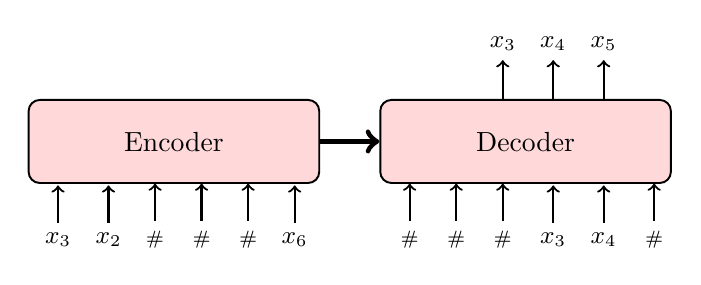
\begin{tikzpicture}
\begin{scope}
\tikzstyle{word} = [font=\scriptsize]
\tikzstyle{model} = [rectangle,draw,minimum height=3em,minimum width=6em,rounded corners=4pt,fill=red!15!white]

\node [anchor=center] (ate) at (0,0) {};

\node [model,minimum width=10.5em,line width=0.7pt] (decoder) at ([xshift=6em]ate.east) {Decoder};
\node [word] (w1) at ([yshift=-2em,xshift=1em]decoder.south) {\small{$x_3$}};
\node [word] (w2) at ([xshift=-1em]w1.west) {\#};
\node [word] (w3) at ([xshift=-1em]w2.west) {\#};
\node [word] (w4) at ([xshift=-1em]w3.west) {\#};
\node [word] (w5) at ([xshift=1em]w1.east) {\small{$x_4$}};
\node [word] (w6) at ([xshift=1em]w5.east) {\#};

\node [word] (w7) at ([yshift=2em,xshift=1em]decoder.north) {\small{$x_4$}};
\node [word] (w8) at ([yshift=0em,xshift=-1em]w7.west) {\small{$x_3$}};
\node [word] (w9) at ([yshift=0em,xshift=1em]w7.east) {\small{$x_5$}};

\draw [->,thick] (w1.north) -- ([yshift=1.35em]w1.north);
\draw [->,thick] (w2.north) -- ([yshift=1.35em]w2.north);
\draw [->,thick] (w3.north) -- ([yshift=1.35em]w3.north);
\draw [->,thick] (w4.north) -- ([yshift=1.35em]w4.north);
\draw [->,thick] (w5.north) -- ([yshift=1.35em]w5.north);
\draw [->,thick] (w6.north) -- ([yshift=1.35em]w6.north);

\draw [->,thick] ([yshift=-1.4em]w7.south) -- (w7.south);
\draw [->,thick] ([yshift=-1.4em]w8.south) -- (w8.south);
\draw [->,thick] ([yshift=-1.4em]w9.south) -- (w9.south);

%encoder
\node [model,minimum width=10.5em,line width=0.7pt] (encoder) at ([xshift=-6em]ate.west) {Encoder};
\node [word] (we1) at ([yshift=-2em,xshift=1em]encoder.south) {\#};
\node [word] (we2) at ([xshift=-1em]we1.west) {\#};
\node [word] (we3) at ([xshift=-1em]we2.west) {\small{$x_2$}};
\node [word] (we4) at ([xshift=-1em]we3.west) {\small{$x_3$}};
\node [word] (we5) at ([xshift=1em]we1.east) {\#};
\node [word] (we6) at ([xshift=1em]we5.east) {\small{$x_6$}};

\draw [->,thick] (we1.north) -- ([yshift=1.35em]we1.north);
\draw [->,thick] (we2.north) -- ([yshift=1.35em]we2.north);
\draw [->,thick] (we3.north) -- ([yshift=1.35em]we3.north);
\draw [->,thick] (we4.north) -- ([yshift=1.35em]we4.north);
\draw [->,thick] (we5.north) -- ([yshift=1.35em]we5.north);
\draw [->,thick] (we6.north) -- ([yshift=1.35em]we6.north);

\draw [->,line width=2pt] ([xshift=0.5em]encoder)--([xshift=-0.5em]decoder);
\end{scope}
\end{tikzpicture}

\caption{MASS 预训练方法}
\label{fig:7-39}
\end{figure}
%-------------------------------------------

\parinterval 以MASS方法为例\cite{song2019mass},可以直接对整个编码器-解码器的结构进行预训练。训练中采用掩码的方式,将源语词序列中的片段替换成特殊词<mask>,然后在解码器端预测这个未知片段,如图\ref{fig:7-39}所示,\#号表示特殊词<mask>。这种做法可以使得编码器端捕捉上下文信息,同时迫使解码器依赖于编码器,学习编码器和解码器之间的注意力进行预训练。而解码器端片段的预测也使得解码器能够学习到向前依赖的上下文表示。

%----------------------------------------------------------------------------------------
%    NEW SUBSUB-SECTION
%----------------------------------------------------------------------------------------

\subsubsection{联合训练}

\parinterval {\small\bfnew{多任务学习}}\index{多任务学习}(Multitask Learning)\index{Multitask Learning}是机器学习的一个子领域,是指同时学习多个独立但是相关的任务\cite{DBLP:journals/corr/Ruder17a}。多任务学习通过模型共享的方式,对多个模型进行学习,而这些模型都对应不同的任务,这样不同模型可以互相``促进''。在神经机器翻译中,为了使用单语数据,可以将翻译任务作为主任务,同时设置一些仅使用单语数据的子任务,通过这些子任务来捕捉单语数据中的语言知识\cite{DBLP:conf/emnlp/DomhanH17}。

\parinterval 语言模型是使用目标端单语数据最直接的方式,但是翻译模型作为一个受限的语言模型,还需要依赖于源语,并不能直接进行多任务学习。针对这个问题,对原有翻译模型结构进行了修改,在解码器中增加了一个语言模型子层,将这个子层用于语言模型任务(图\ref{fig:7-40})。在训练过程中,分别将双语数据和单语数据送入翻译模型和语言模型进行计算,得到的损失相加用于整体模型参数的梯度计算和参数更新,其中语言模型的参数是翻译模型的一部分。

%----------------------------------------------
\begin{figure}[htp]
\centering
\input{./Chapter7/Figures/figure-target-side-multi-task-learning}
\caption{机器翻译中的单任务学习和多任务学习}
\label{fig:7-40}
\end{figure}
%-------------------------------------------

\parinterval 除了多任务学习,还有一些方法将前向模型和反向模型一起训练,在训练过程中同时使用源语言端和目标语言端的单语数据来提升模型性能,双向训练的内容会在\ref{subsection-7.5.4}节中进行介绍。

%----------------------------------------------------------------------------------------
%    NEW SUB-SECTION
%----------------------------------------------------------------------------------------

\subsection{知识精炼}
\label{subsection-7.5.3}

\parinterval 理想的机器翻译系统应该是品质好、速度块、存储占用少。不过现实的机器翻译系统往往需要用运行速度和存储空间来换取翻译品质,比如,\ref{subsection-7.3.2}节提到的增大模型容量的方法就是通过增加模型参数量来达到更好的函数拟合效果,但是这也导致系统变得更加笨拙。在很多场景下,这样的模型甚至无法使用。比如,Transformer-Big等``大''模型通常在专用GPU服务器上运行,在手机等受限环境下仍很难应用。

\parinterval 另一方面,直接训练``小''模型的效果往往并不理想,其翻译品质与``大''模型相比仍有比较明显的差距。比如,在Transformer中,使用一个48层的编码器要比传统的6层编码器在BLEU上高出1-2个点,而且两者翻译结果的人工评价的区别也十分明显。

\parinterval 面对小模型难以训练的问题,一种有趣的想法是把``大''模型的知识传递给``小''模型,让``小''模型可以更好的进行学习。这类似于,教小孩子学习数学,是请一个权威数学家(数据中的标准答案),还是请一个小学数学教师(``大''模型)。这就是知识精炼的基本思想。

%----------------------------------------------------------------------------------------
%    NEW SUBSUB-SECTION
%----------------------------------------------------------------------------------------

\subsubsection{什么是知识精炼}

\parinterval 通常,知识精炼可以被看作是一种知识迁移的手段\cite{Hinton2015Distilling}。如果把``大''模型的知识迁移到``小''模型,这种方法的直接结果就是{\small\bfnew{模型压缩}}\index{模型压缩}(Model Compression)\index{Model Compression}。当然,理论上也可以把``小''模型的知识迁移到``大''模型,比如,将迁移后得到的``大''模型作为初始状态,之后继续训练该模型,以期望取得加速收敛的效果。不过,在实践中更多是使用``大''模型到``小''模型的迁移,这也是本节讨论的重点。

\parinterval 知识精炼基于两个假设:

\begin{itemize}
\vspace{0.5em}
\item ``知识''在模型间是可迁移的。也就是说,一个模型中蕴含的规律可以被另一个模型使用。最典型的例子就是预训练模型(见\ref{subsection-7.2.6})。使用单语数据学习到的表示模型,在双语的翻译任务中仍然可以发挥很好的作用。也就是,把单语语言模型学习到的知识迁移到双语翻译中对句子表示的任务中;
\vspace{0.5em}
\item 模型所蕴含的``知识''比原始数据中的``知识''更容易被学习到。比如,机器翻译中大量使用的回译(伪数据)方法,就把模型的输出作为数据让系统进行学习。
\vspace{0.5em}
\end{itemize}

\parinterval 这里所说的第二个假设对应了机器学习中的一大类问题\ \dash \ {\small\bfnew{学习难度}}\index{学习难度}(Learning Difficulty)\index{Learning Difficulty}。所谓难度是指:在给定一个模型的情况下,需要花费多少代价对目标任务进行学习。如果目标任务很简单,同时模型与任务很匹配,那学习难度就会降低。如果目标任务很复杂,同时模型与其匹配程度很低,那学习难度就会很大。在自然语言处理任务中,这个问题的一种表现是:在很好的数据中学习的模型的翻译质量可能仍然很差。即使训练数据是完美的,但是模型仍然无法做到完美的学习。这可能是因为建模的不合理,导致模型无法描述目标任务中复杂的规律。也就是纵然数据很好,但是模型学不到其中的``知识''。在机器翻译中这个问题体现的尤为明显。比如,在机器翻译系统$n$-best结果中挑选最好的译文(成为Oracle)作为训练样本让系统重新学习,系统仍然达不到Oracle的水平。

\parinterval 知识精炼本身也体现了一种``自学习''的思想。即利用模型(自己)的预测来教模型(自己)。这样既保证了知识可以向更轻量的模型迁移,同时也避免了模型从原始数据中学习难度大的问题。虽然``大''模型的预测中也会有错误,但是这种预测是更符合建模的假设的,因此``小''模型反倒更容易从不完美的信息中学习\footnote[15]{很多时候,``大''模型和``小''模型都是基于同一种架构,因此二者对问题的假设和模型结构都是相似的。}到更多的知识。类似于,刚开始学习围棋的人从职业九段身上可能什么也学不到,但是向一个业余初段的选手学习可能更容易入门。另外,也有研究表明:在机器翻译中,相比于``小''模型,``大''模型更容易进行优化,也更容易找到更好的模型收敛状态。因此在需要一个性能优越,存储较小的模型时,也会考虑将大模型压缩得到更轻量模型的手段\cite{DBLP:journals/corr/abs-2002-11794}。

\parinterval 通常把``大''模型看作的传授知识的``教师'',被称作{\small\bfnew{教师模型}}\index{教师模型}(Teacher Model)\index{Teacher Model};把``小''模型看作是接收知识的``学生'',被称作{\small\bfnew{学生模型}}\index{学生模型}(Student Model)\index{Student Model}。比如,可以把Transformer-Big看作是教师模型,把Transformer-Base看作是学生模型。

%----------------------------------------------------------------------------------------
%    NEW SUBSUB-SECTION
%----------------------------------------------------------------------------------------

\subsubsection{知识精炼的基本方法}

\parinterval 知识精炼的基本思路是让学生模型所表示的函数尽可能去拟合教师模型所表示的函数\cite{Hinton2015Distilling}。通常有两种实现方式\cite{DBLP:conf/emnlp/KimR16}:

\begin{itemize}
\vspace{0.5em}
\item {\small\bfnew{基于单词的知识精炼}}\index{基于单词的知识精炼}(Word-level Knowledge Distillation)\index{Word-level Knowledge Distillation}。该方法的目标是使得学生模型的预测(分布)尽可能逼近教师模型的预测(分布)。令$\mathbf{x}=\{x_1,\ldots,x_m\}$和$\mathbf{y}=\{y_1,\ldots,y_n\}$分别表示输入和输出(数据中的答案)序列,$V$表示目标语言词表,$n$表示译文序列的长度,则基于单词的知识精炼的损失函数被定义为:
\begin{eqnarray}
L_{\textrm{word}} = - \sum_{j=1}^n \sum_{y_j \in V} \textrm{P}_{\textrm{t}} (y_{\textrm{j}}|\mathbf{x})\textrm{logP}_{\textrm{s}}(y_j|\mathbf{x})
\label{eq:7-28}
\end{eqnarray}

这里, $\textrm{P}_{\textrm{s}}(y_j|\mathbf{x})$和$\textrm{P}_{\textrm{t}} (y_i|\mathbf{x})$分别表示学生模型和教师模型在$j$位置的输出的概率。公式\ref{eq:7-28}实际上在最小化教师模型和学生模型输出分布之间的交叉熵。
\vspace{0.5em}
\item {\small\bfnew{基于序列的知识精炼}}\index{基于序列的知识精炼}(Sequence-level Knowledge Distillation)\index{Sequence-level Knowledge Distillation}。除了单词一级的拟合,基于序列的知识精炼希望在序列整体上进行拟合。其损失函数被定义为:
\begin{eqnarray}
L_{\textrm{seq}} = - \sum_{\textrm{y}}\textrm{P}_{\textrm{t}} (\mathbf{y}|\mathbf{x})\textrm{logP}_{\textrm{s}}(\mathbf{y}|\mathbf{x})
\label{eq:7-29}
\end{eqnarray}

公式\ref{eq:7-29}要求遍历所有可能的译文序列,并进行求和,当词表大小为$V$,序列长度为$L$时,则可能的序列的数量有$V$的$L$次幂,这么多的译文将消耗大量的计算资源。因此,会考虑用教师模型的真实输出序列$\hat{\mathbf{y}}$来代替整个空间,即假设$\textrm{P}_{\textrm{t}}(\hat{\mathbf{y}}|\mathbf{x})=1$。于是,目标函数变为:
\begin{eqnarray}
L_{\textrm{seq}} = - \textrm{logP}_{\textrm{s}}(\hat{\mathbf{y}} | \mathbf{x})
\label{eq:7-30}
\end{eqnarray}

这样的损失函数带来最直接的好处是,知识精炼的流程会非常简单。因为只需要利用教师模型将训练数据(源语言)翻译一遍,之后把它的输出替换为训练数据的目标语言部分。之后,利用得到的新的双语数据训练学生模型即可,图\ref{fig:7-41}展示了简化后词级和序列级的不同,其中词级知识精炼的解码端输入为真实双语数据的目标语言,并以teacher模型输出的概率分布作为学习目标,而序列级则直接将teacher推断后得到的结果作为解码端的输入,并将解码结果的One-hot向量作为学习目标。
\vspace{0.5em}
\end{itemize}

%----------------------------------------------
\begin{figure}[htp]
\centering
\input{./Chapter7/Figures/figure-difference-between-word-level-and-sequence-level-in-knowledge-distillation}
\caption{词级和序列级知识精炼的差异}
\label{fig:7-41}
\end{figure}
%-------------------------------------------

\parinterval 本质上,基于单词的知识精炼和传统的语言模型等问题的建模方式是一致的。在传统方法中,训练数据中的答案会被看作是一个One-hot分布,之后让模型去尽可能拟合这种分布。而这里,答案不再是一个One-hot分布,而是由教师模型生成的真实分布,但是损失函数的形式是一模一样的。在具体实现时,一个容易出现的问题是在词级别的知识精炼中,teacher模型的Softmax可能会生成非常尖锐的分布。这时需要考虑对分布进行平滑,提高模型的泛化能力\footnote[16]{比如,可以在Softmax函数中加入一个参数$\alpha$,如$\textrm{Softmax}(s_i)=\frac{exp(s_i/\alpha)}{\sum_j exp(s_i/\alpha)}$。这样可以通过$\alpha$控制分布的平滑程度。
}。

\parinterval 除了在模型最后输出的分布上进行知识精炼,同样可以使用教师模型对学生模型的{\small\bfnew{中间层输出}}\index{中间层输出}(Hint-based Knowledge Transfer)\index{Hint-based Knowledge Transfer}和{\small\bfnew{注意力分布}}\index{注意力分布}(Attention To Attention Transfer)\index{Attention To Attention Transfer}进行约束。而对翻译常用的Transformer架构,也有研究者使用更精细的精炼方式对模型各个位置的知识重新设计了知识迁移的方法\cite{DBLP:journals/corr/abs-1909-10351}。

%----------------------------------------------------------------------------------------
%    NEW SUBSUB-SECTION
%----------------------------------------------------------------------------------------

\subsubsection{机器翻译中的知识精炼}

\parinterval 在神经机器翻译中,通常使用公式\ref{eq:7-30}的方法进行知识精炼,即通过教师模型构造伪数据,之后让学生模型从伪数据中学习。这样做的好处在于,系统研发人员不需要对系统进行任何修改,整个过程只需要调用教师模型和学生模型标准的训练和推断模块即可。

\parinterval 另一个问题是如何构造教师模型和学生模型。以Transformer为例,通常有两种思路:

\begin{itemize}
\vspace{0.5em}
\item 固定教师模型,通过减少模型容量的方式设计学生模型。比如,可以使用容量较大的模型作为教师模型(如:Transformer-Big或Transformer-Deep),然后通过将神经网络变``窄''、变``浅''的方式得到学生模型。我们可以用Transformer-Big做教师模型,然后把Transformer-Big的解码器变为一层网络,作为学生模型。
\vspace{0.5em}
\item 固定学生模型,通过模型集成的方式设计教师模型。可以组合多个模型生成更高质量的译文(见\ref{subsection-7.4.3}节)。比如,融合多个Transformer-Big模型(不同参数初始化方式),之后学习一个Transformer-Base模型。
\vspace{0.5em}
\end{itemize}

\parinterval 此外还可以采用迭代的知识精炼的方式。首先,通过模型集成得到较强的教师模型,再将知识迁移到不同的学生模型上,随后继续使用这些学生模型集成新的教师模型。不断的重复上述过程可以逐步提升集成模型的性能,如图\ref{fig:7-42}所示。值得注意的是,随着迭代次数的增加,集成所带来的收益也会随着子模型之间差异性的减小而减少。

%----------------------------------------------
\begin{figure}[htp]
\centering
\input{./Chapter7/Figures/figure-ensemble-knowledge-distillation}
\caption{迭代式知识精炼}
\label{fig:7-42}
\end{figure}
%-------------------------------------------

\parinterval 如果倾向于使用更少的存储,更快的推理速度,则可以使用更小的学生模型。值得注意的是,对于Transformer模型来说,减少解码端的层数会给推理速度带来巨大的提升。特别是对于基于深层编码器的Transformer-Deep,适当减少解码端层数往往不会带来翻译品质的下降。可以根据不同任务的需求,选择适当大小的学生模型,来平衡存储、推断速度和模型品质之间的关系。

%----------------------------------------------------------------------------------------
%    NEW SUB-SECTION
%----------------------------------------------------------------------------------------

\subsection{双向训练}
\label{subsection-7.5.4}

\parinterval 到目前为止,神经机器翻译系统都是每次一次只训练一个方向的模型。比如,给定中英的双语数据,一次只训练一个中到英或者英到中的翻译系统。既然两个方向的系统都使用同样的双语数据进行训练,那么是否可以一次训练同时得到两个方向的翻译系统呢?

\parinterval 回顾神经机器翻译系统的建模过程,给定一个互译的句对$(\mathbf s,\mathbf t)$,一个从源语言句子$\mathbf s$到目标语言句子$\mathbf t$的翻译被表示为求条件概率$\textrm{P}(\mathbf t|\mathbf s)$的问题。类似地,一个从目标语言句子$\mathbf t$到源语言句子$\mathbf s$的翻译可以表示为$\textrm{P}(\mathbf s|\mathbf t)$。通常来说,神经机器翻译的训练一次只得到一个方向的模型,也就是$\textrm{P}(\mathbf t|\mathbf s)$或者$\textrm{P}(\mathbf s|\mathbf t)$。这意味着$\textrm{P}(\mathbf t|\mathbf s)$和$\textrm{P}(\mathbf s|\mathbf t)$之间是互相独立的。$\textrm{P}(\mathbf t|\mathbf s)$和$\textrm{P}(\mathbf s|\mathbf t)$是否真的没有关系呢?比如,$\mathbf s$和$\mathbf t$是相同大小的向量,且$\mathbf s$到$\mathbf t$的变换是一个线性变换,也就是与一个方阵$\mathbf{W}$做矩阵乘法:

\begin{eqnarray}
\mathbf t = \mathbf s \cdot \mathbf{W}
\label{eq:7-31}
\end{eqnarray}

\parinterval 这里可以把$\mathbf s$和$\mathbf t$都看作分布式的向量表示;$\mathbf{W}$应当是一个满秩矩阵,否则对于任意一个$\mathbf s$经过$\mathbf{W}$变换得到的$\mathbf t$只落在所有可能的$\mathbf t$的一个子空间内,即在给定$\mathbf{W}$的情况下有些$\mathbf t$不能被任何一个$\mathbf s$表达,而这不符合常识,因为不管是什么句子,我们总能找到它的一种译文。若$\mathbf{W}$是满秩矩阵说明$\mathbf{W}$可逆,也就是给定$\mathbf s$到$\mathbf t$的变换$\mathbf{W}$下,$\mathbf t$到$\mathbf s$的变换必然是$\mathbf{W}$的逆而不是其他矩阵。这个例子说明$\textrm{P}(\mathbf t|\mathbf s)$和$\textrm{P}(\mathbf s|\mathbf t)$直觉上应当存在联系。当然,$\mathbf s$和$\mathbf t$之间是否存在简单的线性变换关系并没有结论,但是上面的例子给出了一种对源语言句子和目标语言句子进行相互转化的思路。实际上,研究人员已经通过一些数学技巧用目标函数来把$\textrm{P}(\mathbf t|\mathbf s)$和$\textrm{P}(\mathbf s|\mathbf t)$联系起来,这样训练神经机器翻译系统一次就可以同时得到两个方向的翻译模型,使得训练变得更加高效\cite{Hassan2018AchievingHP}。

%----------------------------------------------------------------------------------------
%    NEW SUBSUB-SECTION
%----------------------------------------------------------------------------------------

\subsubsection{有监督对偶学习}

\parinterval 除了用条件概率$\textrm{P}(\mathbf t|\mathbf s)$建模翻译问题,还可以使用联合分布$\textrm{P}(\mathbf s,\mathbf t)$进行建模\cite{DBLP:conf/icml/XiaQCBYL17}。根据条件概率的定义,有:
\begin{eqnarray}
\textrm{P}(\mathbf s,\mathbf t) &=& \textrm{P}(\mathbf s)\textrm{P}(\mathbf t|\mathbf s) \nonumber \\
&=& \textrm{P}(t)\textrm{P}(\mathbf s|\mathbf t)
\label{eq:7-32}
\end{eqnarray}

\parinterval 公式\ref{eq:7-32}很自然地把两个方向的翻译模型$\textrm{P}(\mathbf t|\mathbf s)$和$\textrm{P}(\mathbf s|\mathbf t)$以及两个语言模型$\textrm{P}(\mathbf s)$和$\textrm{P}(\mathbf t)$联系起来:$\textrm{P}(\mathbf s)\textrm{P}(\mathbf t|\mathbf s)$应该与$\textrm{P}(\mathbf t)\textrm{P}(\mathbf s|\mathbf t)$接近,因为它们都表达了同一个联合分布$\textrm{P}(\mathbf s,\mathbf t)$。因此,在构建训练两个方向的翻译模型的目标函数时,除了它们单独训练时各自使用的极大似然估计目标函数,可以额外增加一个目标项来鼓励两个方向的翻译模型去满足公式\ref{eq:7-32}:
\begin{eqnarray}
\mathcal{L} = (\textrm{log P}(\mathbf s) + \textrm{log P}(\mathbf t|\mathbf s) - \textrm{log P}(\mathbf t) - \textrm{log P}(\mathbf s|\mathbf t))^{2}
\label{eq:7-33}
\end{eqnarray}

\parinterval 其中$\textrm{P}(\mathbf s)$和$\textrm{P}(\mathbf t)$这两个语言模型是预先训练好的,并不参与翻译模型的训练。可以看到,对于单独的一个模型来说,其目标函数增加了与另外一个方向的模型相关的项。这样的形式与L1/L2正则化非常类似(见\ref{subsection-7.3.1}节),因此可以把这个方法看作是一种任务特定的正则化的手段(由翻译任务本身的性质所启发而来)。由于两个方向的翻译模型和语言模型相互影响,这种方法能得到比基于单个方向训练效果更好的模型。

%----------------------------------------------------------------------------------------
%    NEW SUBSUB-SECTION
%----------------------------------------------------------------------------------------

\subsubsection{无监督对偶学习}

\parinterval 在有监督对偶学习对联合分布$\textrm{P}(\mathbf s,\mathbf t)$建模的基础上,如果把$\mathbf  t$看作一个隐变量,那么可以得到边缘分布$\textrm{P}(\mathbf s)$,也就是关于$\mathbf s$的语言模型:
\begin{eqnarray}
\textrm{P}(\mathbf s) &=& \sum_{\mathbf t}\textrm{P}(\mathbf s,\mathbf t) \nonumber \\
&=& \sum_{\mathbf t}\textrm{P}(\mathbf s|\mathbf t)\textrm{P}(\mathbf t|\mathbf s)
\label{eq:7-34}
\end{eqnarray}

\noindent  公式\ref{eq:7-34}假设$\textrm{P}(\mathbf s|\mathbf t)=\textrm{P}(\mathbf s|\mathbf s,\mathbf t)$。这个假设显然是成立的,因为当知道一个句子的译文时,并不需要知道它的源文就可以把它翻译回去。如果直接优化(最大化)公式\ref{eq:7-34}右侧,相当于对这个等式$\textrm{P}(\mathbf s|\mathbf t)$和$\textrm{P}(\mathbf t|\mathbf s)$施加了{\small\bfnew{循环一致性}}\index{循环一致性}(Circle Consistency)\index{Circle Consistency}的约束\cite{DBLP:conf/iccv/ZhuPIE17},也就是对于一个句子$\mathbf s$,通过$\textrm{P}(\mathbf t|\mathbf s)$把它翻译成$\mathbf t$后,根据$\textrm{P}(\mathbf s|\mathbf t)$应该能重新翻译出$\mathbf s$,如图\ref{fig:7-43}所示。公式\ref{eq:7-34}给出了同时优化$\textrm{P}(\mathbf s|\mathbf t)$和$\textrm{P}(\mathbf t|\mathbf s)$的一个目标函数形式。这个目标函数的一个额外的好处是它本质上是在学习一个由$\textrm{P}(\mathbf s|\mathbf t)$和$\textrm{P}(\mathbf t|\mathbf s)$组成的语言模型$\textrm{P}(\mathbf s)$,而$\textrm{P}(\mathbf s)$的学习依赖于单语数据,这意味着这个目标函数可以很自然地直接使用大量单语数据来同时训练两个翻译模型。相同的结论可以推广到$\textrm{P}(\mathbf t)$上\cite{DBLP:conf/nips/HeXQWYLM16}。

%----------------------------------------------
\begin{figure}[htp]
\centering
\input{./Chapter7/Figures/figure-cycle-consistency}
\caption{循环一致性}
\label{fig:7-43}
\end{figure}
%----------------------------------------------

\parinterval 但是直接使用公式\ref{eq:7-34}作为目标函数需要解决两个问题:

\begin{itemize}
\vspace{0.5em}
\item 计算公式\ref{eq:7-34}要枚举所有可能的隐变量$\mathbf t$的取值,也就是所有可能产生的目标语句子,而这是不可能的,因此一般会通过平均多个随机产生的$\mathbf t$对应的损失来近似真正的目标函数值;
\vspace{0.5em}
\item 从公式\ref{eq:7-34}可以看到,在$\textrm{P}(\mathbf s)$上计算完目标函数值后,得到的梯度首先传递给$\textrm{P}(\mathbf s|\mathbf t)$,然后通过$\textrm{P}(\mathbf s|\mathbf t)$传递给$\textrm{P}(\mathbf t|\mathbf s)$。由于$\textrm{P}(\mathbf s|\mathbf t)$的输入$\mathbf t$由$\textrm{P}(\mathbf t|\mathbf s)$采样得到,而采样操作不可导,导致梯度的传播在$\textrm{P}(\mathbf t|\mathbf s)$的输出处断开了,因此$\textrm{P}(\mathbf t|\mathbf s)$接收不到任何梯度来进行更新。常见的解决方案是使用策略梯度\cite{DBLP:conf/nips/SuttonMSM99}。它把$\textrm{P}(\mathbf t|\mathbf s)$采样得到的$\mathbf t$当成$\textrm{P}(\mathbf t|\mathbf s)$的目标来学习,并使用$\textrm{log P}(\mathbf s|\mathbf t)$对$\textrm{P}(\mathbf t|\mathbf s)$的损失进行加权。但是由于仅使用少量样本来近似真正的目标函数,得到的策略梯度方差非常大,系统无法稳定学习,特别是训练的初期,因此通常会需要先使用双语数据预训练两个方向的翻译模型,然后把公式\ref{eq:7-34}作为正常训练的一个正则化项使用。
\vspace{0.5em}
\end{itemize}

%----------------------------------------------------------------------------------------
%    NEW SUBSUB-SECTION
%----------------------------------------------------------------------------------------

\subsubsection{翻译中回译}

\parinterval 重新回顾公式\ref{eq:7-34}对应的目标函数,无监督对偶学习跟回译(假设现在只在一个句对$(\mathbf s,\mathbf t)$上做回译)之间有着很深的内在联系:给定一个句子$\mathbf s$,无监督对偶学习和回译都首先用$\textrm{P}(\mathbf t|\mathbf s)$把$\mathbf s$翻译成$\mathbf t$,然后无监督对偶学习最大化$\textrm{P}(\mathbf s|\mathbf t)\textrm{P}(\mathbf t|\mathbf s)$,而回译则是最大化$\textrm{P}(\mathbf s|\mathbf t)$。可以看到,当无监督对偶学习假设$\textrm{P}(\mathbf t|\mathbf s)$是一个完美的翻译模型的时候,它与回译是等价的。此外,在共享两个方向的模型参数$\theta$的情况下,可以看到无监督对偶学习的梯度为$\frac{\partial \textrm{P}(\mathbf s)}{\partial \theta} =\textrm{P}(\mathbf t|\mathbf s) \frac{\partial \textrm{P}(\mathbf s|\mathbf t)}{\partial \theta}+\textrm{P}(\mathbf s|\mathbf t) \frac{\partial \textrm{P}(\mathbf t|\mathbf s)}{\partial \theta} $,而回译的梯度为$\frac{\partial \textrm{P}(\mathbf s|\mathbf t)}{\partial \theta}$。从这个角度出发,无监督对偶学习与回译都在优化语言模型$\textrm{P}(\mathbf s)$这个目标函数,只不过回译使用对$\theta$有偏的梯度估计。

\parinterval 这个事实说明对回译进行适当的增广后应该能取得与无监督对偶学习相似的结果。{\small\bfnew{ 翻译中回译}}\index{翻译中回译}(On-the-fly Back-translation)\index{On-the-fly Back-translation}就是这样一个例子。一般回译的过程是先把数据集里所有$\mathbf s$都翻译出来,然后只训练$\textrm{P}(\mathbf s|\mathbf t)$。区别于回译,从数据集中采集到一个$\mathbf s$之后,翻译中回译立刻把$\mathbf s$翻译成$\mathbf t$,然后训练$\textrm{P}(\mathbf s|\mathbf t)$,并且在下一步迭代中采集一个$\mathbf t$然后训练$\textrm{P}(\mathbf t|\mathbf s)$,这样交替更新$\textrm{P}(\mathbf s|\mathbf t)$和$\textrm{P}(\mathbf t|\mathbf s)$。尽管翻译中回译无法像无监督对偶学习那样在一个样本里通过梯度把$\textrm{P}(\mathbf s|\mathbf t)$的信息传到$\textrm{P}(\mathbf t|\mathbf s)$,但是它交替更新$\textrm{P}(\mathbf s|\mathbf t)$和$\textrm{P}(\mathbf t|\mathbf s)$的策略允许$\textrm{P}(\mathbf s|\mathbf t)$在两个样本间通过其产生的输出$\mathbf s$来把信息传递到$\textrm{P}(\mathbf t|\mathbf s)$,因此也能获得相近的效果,并且在实现和计算上都非常高效。翻译中回译已经在无监督神经机器翻译系统训练中被广泛使用\cite{lample2019cross}。

%----------------------------------------------------------------------------------------
%    NEW SECTION
%----------------------------------------------------------------------------------------

\sectionnewpage
\section{小结及深入阅读}

\parinterval 神经机器翻译的模型和技术方法已经十分丰富,无论是对基础问题的研究,还是研发实际可用的系统,人们都会面临很多选择。本章,从构建一个足以参加机器翻译比赛的系统出发,对神经机器翻译的数据处理、建模与训练、推断等基本问题进行了介绍。其中的许多方法已经在实践中得到验证,具有较好的参考意义。此外,本章也对一些前沿方法进行了讨论,旨在挖掘更具潜力的方向。

\parinterval 除了以上内容,还有一些方向值得关注:

\begin{itemize}
\vspace{0.5em}
\item 无指导机器翻译。无指导机器翻译由于其不需要双语语料即可训练翻译模型的特性,在稀缺资源机器翻译的场景中有非常大的潜力而得到广泛的关注。目前无指导机器翻译主要有两种范式:第一种先得到词典的翻译,然后得到短语表的翻译和相应的统计机器翻译系统,最后使用统计机器翻译系统生成伪双语平行语料训练神经机器翻译系统\cite{DBLP:conf/acl/ArtetxeLA19};第二种是先预训练语言模型来初始化神经机器翻译系统的编码器和解码器,然后使用翻译中回译以及降噪自编码器来训练神经机器翻译系统\cite{lample2019cross}。尽管目前无指导机器翻译在富资源的语种上取得了很大进展,但是离实际应用还有很远距离。比如,目前无指导系统都依赖于大量单语数据,而实际上稀缺资源的语种不但双语语料少,单语语料也少;此外,这些系统还无法在远距离如中英这些字母表重合少,需要大范围调序的语种对上取得可接受的结果;使用大量单语训练无指导系统还面临数据来自于不同领域的问题\cite{DBLP:journals/corr/abs-2004-05516}。设计更鲁棒,使用单语数据更高效的无指导机器翻译方法乃至新范式会是未来的趋势。
\vspace{0.5em}
\item 图片翻译。由于人类语言潜在的歧义性,传统的神经机器翻译在单句翻译中可能会出现歧义。为此,一些研究工作在翻译过程中尝试引入更多的上下文信息,比如多模态翻译、基于树的翻译或者篇章级翻译。比如,图片翻译的目标就是在给定一个图片和其源语描述的情况下,生成目标语言的描述。一般做法就是通过一个额外的编码器来提取图像特征\cite{DBLP:journals/corr/ElliottFH15,DBLP:conf/acl/HitschlerSR16},然后通过权重门控机制、注意力网络等融合到系统中\cite{DBLP:conf/wmt/HuangLSOD16}。

\vspace{0.5em}
\item 基于树的翻译。这类方法在翻译模型中引入句法结构树或依存树,从而引入更多的句法信息。一种常用的做法是将句法树进行序列化,从而保留序列到序列的模型结构\cite{DBLP:conf/emnlp/CurreyH18,DBLP:conf/acl/SaundersSGB18}。在此基础上,一些研究工作引入了更多的解析结果\cite{DBLP:conf/acl/SumitaUZTM18,DBLP:conf/coling/ZaremoodiH18}。同时,也有一些研究工作直接使用Tree-LSTMs等网络结构\cite{DBLP:conf/acl/TaiSM15,DBLP:conf/iclr/ShenTSC19}来直接表示树结构,并将其应用到神经机器翻译模型中\cite{DBLP:conf/acl/EriguchiHT16,Yang2017TowardsBH,DBLP:conf/acl/ChenHCC17}。

\vspace{0.5em}
\item 篇章级翻译。可以通过引入篇章级上下文信息,来处理篇章翻译中译文不连贯,主谓不一致等问题。为此,一些研究人员针对该问题进行了改进,主要可以分为两类方法:一种是将当前句子与上下文进行句子级的拼接,不改变模型的结构\cite{DBLP:conf/discomt/TiedemannS17},另外一种是采用额外的编码器来捕获篇章信息\cite{DBLP:journals/corr/JeanLFC17,DBLP:journals/corr/abs-1805-10163,DBLP:conf/emnlp/ZhangLSZXZL18}。编码器的结构除了传统的RNN、自注意力网络,还有利用层级注意力来编码之前的多句上文\cite{Werlen2018DocumentLevelNM,tan-etal-2019-hierarchical},使用可选择的稀疏注意力机制对整个文档进行篇章建模\cite{DBLP:conf/naacl/MarufMH19},使用记忆网络、缓存机制等对篇章中的关键词进行提取\cite{DBLP:conf/coling/KuangXLZ18,DBLP:journals/tacl/TuLSZ18}或者采用两阶段解码的方式\cite{DBLP:conf/aaai/XiongH0W19,DBLP:conf/acl/VoitaST19}。除了从建模角度引入上下文信息,也有一些工作使用篇章级修正模型\cite{DBLP:conf/emnlp/VoitaST19}或者语言模型\cite{DBLP:journals/corr/abs-1910-00553}对句子级翻译模型的译文进行修正,或者通过自学习在解码过程中保持翻译连贯性\cite{DBLP:journals/corr/abs-2003-05259}。
\vspace{0.5em}
\item 语音翻译。在日常生活中,语音翻译也是有很大的需求。针对语音到文本翻译的特点,最简单的做法是使用自动语音识别(ASR)将语音转换成文本,然后送入文本翻译模型进行翻译\cite{DBLP:conf/icassp/Ney99,DBLP:conf/interspeech/MatusovKN05}。然而为了避免流水线中的错误传播和高延迟问题,现在通常采用端到端的建模做法\cite{DBLP:conf/naacl/DuongACBC16,DBLP:journals/corr/BerardPSB16}。同时,针对语音翻译数据稀缺的问题,一些研究工作采用各种方法来进行缓解,包括预训练\cite{DBLP:conf/naacl/BansalKLLG19}、多任务学习\cite{Weiss2017SequencetoSequenceMC,DBLP:conf/icassp/BerardBKP18}、课程学习\cite{DBLP:conf/interspeech/KanoS017}、注意力传递\cite{DBLP:journals/tacl/SperberNNW19}和知识精炼\cite{DBLP:conf/interspeech/LiuXZHWWZ19,DBLP:conf/icassp/JiaJMWCCALW19}。
\vspace{0.5em}
\item 多语言翻译。神经机器翻译模型经过训练,通常可以将一种固定的源语言翻译成另一种固定的目标语言,但考虑到世界上有成千上万种语言,为每种语言对训练一个单独的模型非常耗资源\cite{DBLP:journals/tacl/JohnsonSLKWCTVW17}。多语言神经机器翻译旨在训练涵盖多种语言翻译的单一模型。多语言神经机器翻译系统可以根据它们在不同翻译语言对之间共享的组件进行分类。一种常见的做法是通过语言标签指定源语言和目标语言的同时,共享整个神经网络结构(编码器和解码器)\cite{DBLP:journals/corr/HaNW16,DBLP:journals/tacl/JohnsonSLKWCTVW17}。除此之外,还可以共享部分网络结构。比如共享编码器的一对多模型\cite{dong-etal-2015-multi},共享解码器的多对一模型\cite{firat-etal-2016-zero,Zoph2016MultiSourceNT},以及共享注意力机制的多对多模型\cite{DBLP:journals/corr/LuongLSVK15,DBLP:conf/naacl/FiratCB16}。多语言神经机器翻译不仅可以减少训练单一语言对神经机器翻译的训练代价,还可以有效的解决零资源神经机器翻译\cite{DBLP:journals/tacl/JohnsonSLKWCTVW17}以及多源神经机器翻译问题\cite{Och01statisticalmulti-source}。
\vspace{0.5em}
\item 结构搜索。除了由研究人员手工设计神经网络结构之外,近些年{\small\bfnew{网络结构搜索技术}}\index{网络结构搜索技术}(Neural Architecture Search;NAS)\index{Neural Architecture Search;NAS}也逐渐在包括机器翻译在内的自然语言处理任务中得到广泛关注\cite{elsken2019neural}。不同于前文提到的基于循环神经网络、Transformer结构的机器翻译模型,网络结构搜索旨在通过自动的方式根据提供的训练数据自动学习到最适合于当前任务的神经网络模型结构。目前而言,网络结构搜索的方法已经在自然语言处理的各项任务中崭露头角,在语言模型、命名实体识别等任务中获得优异的成绩\cite{DBLP:conf/iclr/ZophL17,DBLP:conf/emnlp/JiangHXZZ19,liyinqiaoESS},但对于机器翻译任务而言,由于其任务的复杂性,网络结构的搜索空间往往比较大,很难直接对其空间进行搜索,因此研究人员更倾向于对基于现有经验设计的模型结构进行改良。谷歌大脑团队在The Evolved Transformer文章中提出使用进化算法,在Transformer结构基础上对模型结构进行演化,得到更加高效且建模能力更强的机器翻译模型。微软团队也在Neural Architecture Optimization\cite{DBLP:conf/nips/LuoTQCL18}论文中提出NAO的方法,通过将神经网络结构映射到连续空间上进行优化来获得优于初始结构的模型,NAO方法在WMT19机器翻译评测任务中也进行了使用,在英语-芬兰语以及芬兰语-英语的任务上均取得了优异的成绩。
\vspace{0.5em}
\item 与统计机器翻译的结合。尽管神经机器翻译在自动评价和人工评价上都取得比统计机器翻译优异的结果,但神经机器翻译仍然面临一些统计机器翻译没有的问题\cite{DBLP:conf/aclnmt/KoehnK17},如神经机器翻译系统会产生漏译的现象,也就是源语句子的一些短语甚至从句没有被翻译,而统计机器翻译因为是把源语里所有短语都翻译出来后进行拼装,因此不会产生这种译文对原文的忠实度低的问题。一个解决的思路就是把统计机器翻译系统和神经机器翻译系统进行结合。目前的方法主要分为两种,一种是模型的改进,比如在神经机器翻译里建模统计机器翻译的概念或者使用统计机器翻译系统的模块,如词对齐,覆盖度等等\cite{DBLP:conf/aaai/HeHWW16},或者是把神经机器翻译系统结合到统计机器翻译系统中,如作为一个特征\cite{DBLP:conf/aclwat/NeubigMN15};第二种是系统融合,在不改变模型的情况下,把来自神经机器翻译系统的输出和统计机器翻译系统的输出进行融合,得到更好的结果,如使用重排序\cite{DBLP:conf/ijcnlp/KhayrallahKDPK17,DBLP:conf/aclwat/NeubigMN15},后处理\cite{niehues-etal-2016-pre},或者把统计机器翻译系统的输出作为神经机器翻译系统解码的约束条件等等\cite{DBLP:conf/eacl/GispertBHS17}。除此之外,也可以把神经机器翻译与翻译记忆相融合\cite{DBLP:conf/aaai/XiaHLS19,DBLP:conf/nlpcc/HeHLL19},这在机器翻译应用中也是非常有趣的方向。
\end{itemize}












